	% =======================================================
	%                 第 11 章：有市场势力的定价
	% =======================================================
	\chapter{有市场势力的定价}
	
	\section{复习题}
	\begin{enumerate}[label=\textbf{\arabic*.}, leftmargin=*]
		\item \textbf{假设某厂商能实行完全的一级价格歧视。它会定的最低价格是什么？它的总产量是什么？}
		
		\textbf{答：}
		厂商会定的最低价格等于其最后生产单位的边际成本，总产量则等于完全竞争市场下的有效产量水平。
		
		首先，在完全的一级价格歧视下，厂商能够向每位消费者索取其愿意支付的最高保留价格，此时其面临的边际收益曲线与市场需求曲线完全重合（即 $MR=D$）。
		
		由于价格歧视策略并不改变厂商的基础成本结构，厂商为了实现利润最大化，将持续扩大产量，直到销售额外单位所带来的边际收益等于生产该单位的边际成本。
		
		如图所示，厂商的生产决策点位于需求曲线与边际成本曲线的交点，此时对应的总产量为 $Q$，边际消费者支付的最低价格为 $P$。在该均衡状态下，无谓损失被完全消除，厂商将原本的消费者剩余全部榨取并转化为图中标注的剥夺区域 $A$ 的可变利润。
		
		\begin{center}
			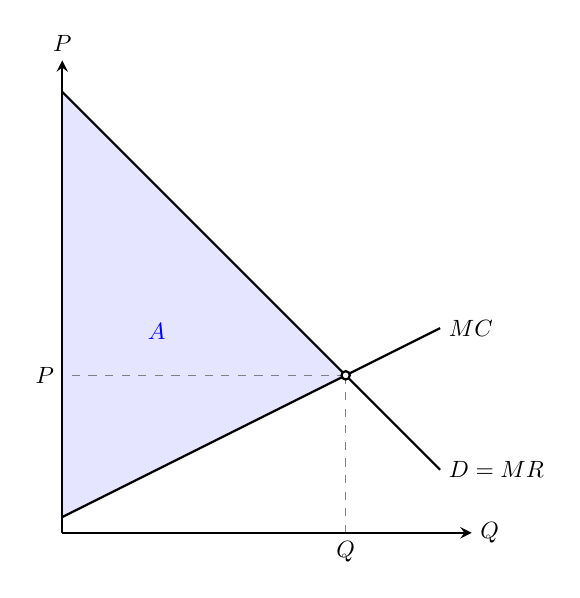
\begin{tikzpicture}[x=0.8cm, y=0.8cm, >=stealth, thick, every node/.style={scale=0.85}]
				\coordinate (E) at (4.5, 2.5);
				
				% 1. 福利或剩余区域填充 (最底层)
				\fill[blue!10] (0, 7) -- (E) -- (0, 0.25) -- cycle;
				\node[blue] at (1.5, 3.2) {$A$};
				
				% 2. 辅助虚线
				\draw[dashed, thin, gray] (E) -- (4.5, 0) node[below, text=black] {$Q$};
				\draw[dashed, thin, gray] (E) -- (0, 2.5) node[left, text=black] {$P$};
				
				% 3. 坐标轴
				\draw[->] (0,0) -- (6.5,0) node[right] {$Q$};
				\draw[->] (0,0) -- (0,7.5) node[above] {$P$};
				
				% 4. 绘图代码
				\draw[domain=0:6, color=black] plot (\x, {7 - \x}) node[right] {$D=MR$};
				\draw[domain=0:6, color=black] plot (\x, {0.25 + 0.5*\x}) node[right] {$MC$};
				
				% 5. 均衡点与标号
				\fill[white] (E) circle (1.5pt);
				\draw (E) circle (1.5pt);
			\end{tikzpicture}
		\end{center}
		
		\item \textbf{汽车推销员是怎样实行价格歧视的？正确利用价格歧视的能力是怎样影响他的收入的？}
		
		\textbf{答：}
		推销员主要通过在议价过程中甄别消费者的保留价格和需求价格弹性来实现近似的一级价格歧视。
		
		首先，推销员利用信息不对称，以厂商建议的标价作为初始索价上限，随后通过观察和试探消费者的搜寻成本、耐心程度及购买意愿，动态决定让利幅度。
		
		对于搜寻成本高、缺乏耐心或急于购车的消费者（呈现低需求弹性），推销员给予极少折扣甚至维持原价；而对于明确表示可能转向竞争品牌、对价格极为敏感的消费者（呈现高需求弹性），推销员则提供较大幅度的折扣以促成交易。
		
		这种甄别能力使得推销员能够根据个体的边际支付意愿进行“量体裁衣”式的定价，从而最大程度地榨取消费者剩余并将其转化为自身的销售佣金，因此其精准实施价格歧视的能力与个人收入呈现高度的的正相关。
		
		\item \textbf{电力事业公司常常实行二级价格歧视。为什么这可能会改善消费者的福利？}
		
		\textbf{答：}
		电力公司通过对不同消费量区段制定阶梯式费率（即分段定价）实施二级价格歧视，此举通过产量扩张效应改善了整体福利水平。
		
		电力等公共事业通常具备显著的规模经济特征，其长期平均成本（$AC$）与边际成本（$MC$）在有效市场需求范围内随产量增加而递减。若强制实行单一垄断定价（如 $P_1$），厂商为了维持高额利润会严重限制产量，导致大量低支付意愿消费者被挤出市场。而在二级价格歧视下，厂商将价格结构分段（第一区段索价 $P_1$，第二区段索价 $P_2$），不仅继续从高需求量消费者处榨取利润，同时也将产品边际延伸至对价格敏感的低收入群体。
		
		如图所示，实行分段定价后，第一区段的消费者保留了面积为 $CS_1$ 的消费者剩余，而原本被高价排斥的消费者现在能够以较低的 $P_2$ 进行购买，从而获得了原本不存在的新增剩余 $CS_2$。这种机制在提升厂商总利润的同时，使总产出向竞争均衡逼近，有效削减了无谓损失并实质性地增进了社会总福利。
		
		\begin{center}
			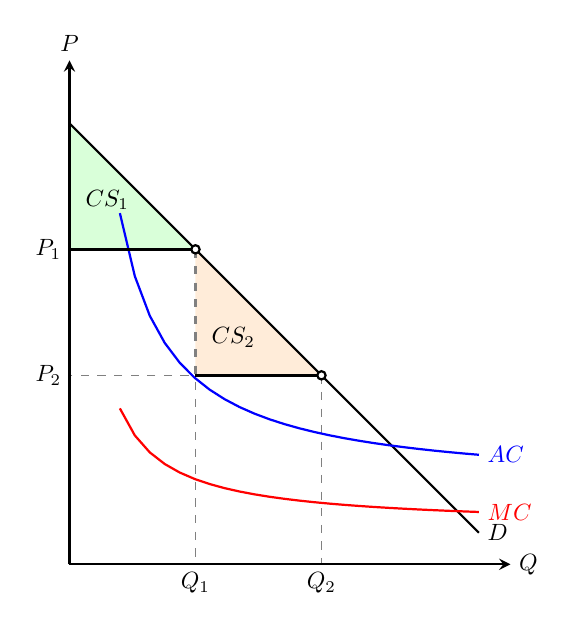
\begin{tikzpicture}[x=0.8cm, y=0.8cm, >=stealth, thick, every node/.style={scale=0.85}]
				% 1. 福利或剩余区域填充 (最底层)
				\fill[green!15] (0, 7) -- (0, 5) -- (2, 5) -- cycle;
				\fill[orange!15] (2, 5) -- (2, 3) -- (4, 3) -- cycle;
				
				% 2. 辅助虚线
				\draw[dashed, thin, gray] (2, 5) -- (2, 0) node[below, text=black] {$Q_1$};
				\draw[dashed, thin, gray] (2, 5) -- (0, 5) node[left, text=black] {$P_1$};
				\draw[dashed, thin, gray] (4, 3) -- (4, 0) node[below, text=black] {$Q_2$};
				\draw[dashed, thin, gray] (4, 3) -- (0, 3) node[left, text=black] {$P_2$};
				
				% 3. 坐标轴
				\draw[->] (0,0) -- (7,0) node[right] {$Q$};
				\draw[->] (0,0) -- (0,8) node[above] {$P$};
				
				% 4. 绘图代码
				\draw[domain=0:6.5, color=black] plot (\x, {7 - \x}) node[right] {$D$};
				\draw[domain=0.8:6.5, color=blue] plot (\x, {3.5/\x + 1.2}) node[right] {$AC$};
				\draw[domain=0.8:6.5, color=red] plot (\x, {1.5/\x + 0.6}) node[right] {$MC$};
				
				% 分段定价阶梯线
				\draw[very thick] (0, 5) -- (2, 5);
				\draw[dashed, thick, gray] (2, 5) -- (2, 3);
				\draw[very thick] (2, 3) -- (4, 3);
				
				% 5. 标号
				\node[yshift=5pt] at (0.6, 5.6) {$CS_1$};
				\node at (2.6, 3.6) {$CS_2$};
				
				\fill[white] (2, 5) circle (1.5pt);
				\draw (2, 5) circle (1.5pt);
				\fill[white] (4, 3) circle (1.5pt);
				\draw (4, 3) circle (1.5pt);
			\end{tikzpicture}
		\end{center}
		
		\item \textbf{给出一些三级价格歧视的例子。如果不同的消费群体有不同的需求水平但有相同的价格弹性，三级价格歧视会是有效的吗？}
		
		\textbf{答：}
		三级价格歧视是指垄断厂商将消费者划分为具有不同需求曲线的独立群体，并根据各群体的需求价格弹性分别索取不同价格的定价策略。常见的应用场景包括：针对学生和老年人的电影票或景点门票折扣、航空公司的全价与特价机票、软件的商业版与教育版定价，以及针对不同时段的公共交通错峰费率。
		
		如果不同的消费群体虽然需求水平不同，但具有完全相同的需求价格弹性，三级价格歧视将失去效用并退化为单一价格垄断。根据利润最大化条件，厂商在不同市场中分配产量的原则是使各市场的边际收益相等，即：
		\[
		\begin{aligned}
			MR_1 = MR_2
		\end{aligned}
		\]
		
		根据边际收益与价格弹性的代数关系，该条件可等价转换为：
		\[
		\begin{aligned}
			P_1 \left( 1 + \frac{1}{E_1} \right) = P_2 \left( 1 + \frac{1}{E_2} \right)
		\end{aligned}
		\]
		
		将其整理为价格比率的形式：
		\[
		\begin{aligned}
			\frac{P_1}{P_2} = \frac{1 + 1/E_2}{1 + 1/E_1}
		\end{aligned}
		\]
		
		在此方程中，若两个市场的需求价格弹性严格相等（$E_1 = E_2$），等式右侧将等于 1，必然推导出 $P_1 = P_2$。这意味着厂商的最优决策是对两个群体索取完全相同的价格，试图实施价格歧视既无法增加利润，也无任何实际意义。
		
		\item \textbf{说明为什么最优的三级价格歧视要求对各消费者群体的边际收益等于边际成本。用这个条件解释当一个消费群体的需求曲线外移，从而对该群体的边际收益增加时，厂商应怎样变动它的价格和总产量。}
		
		\textbf{答：}
		实现最优的三级价格歧视必须同时满足两个边际条件。各独立市场的边际收益必须相互相等（$MR_1 = MR_2$）。如果某一市场的边际收益更高，厂商在不改变总成本的前提下，只需将一单位产量从低边际收益市场转移至高边际收益市场，即可获得纯增量利润，直至两者的边际收益被拉平。统一的边际收益必须严格等于厂商生产总产量的边际成本（$MR_1 = MR_2 = MC$）。如果统一的边际收益大于边际成本，扩大总产量能继续增加利润；若小于边际成本，则必须缩减总产量。
		
		当消费群体 1 的需求曲线发生外移时，其对应的边际收益曲线 $MR_1$ 会同步向右平移。在初始的均衡产量下，这会打破原有的等式，导致 $MR_1$ 瞬间大于 $MR_2$ 且大于 $MC$。为了捕获新增的利润空间，厂商会增加对群体 1 的产量供应。
		
		这种总产量的扩张会导致厂商沿着向上倾斜的边际成本曲线移动，使得全局均衡边际成本（$MC$）被推高。为了在更高的边际成本水平上重新建立 $MR_1 = MR_2 = MC$ 的均衡，厂商必须对消费群体 2 进行被动调整。由于群体 2 的需求曲线并未改变，为了使其边际收益 $MR_2$ 提升至新的、更高的 $MC$ 水平，厂商必须削减投放至群体 2 的产量并相应地提高其价格。总体而言，厂商将扩大总产量，增加群体 1 的供给并视需求变动形态调整其价格，同时必然缩减群体 2 的供给并提高其价格。
		
		\begin{center}
			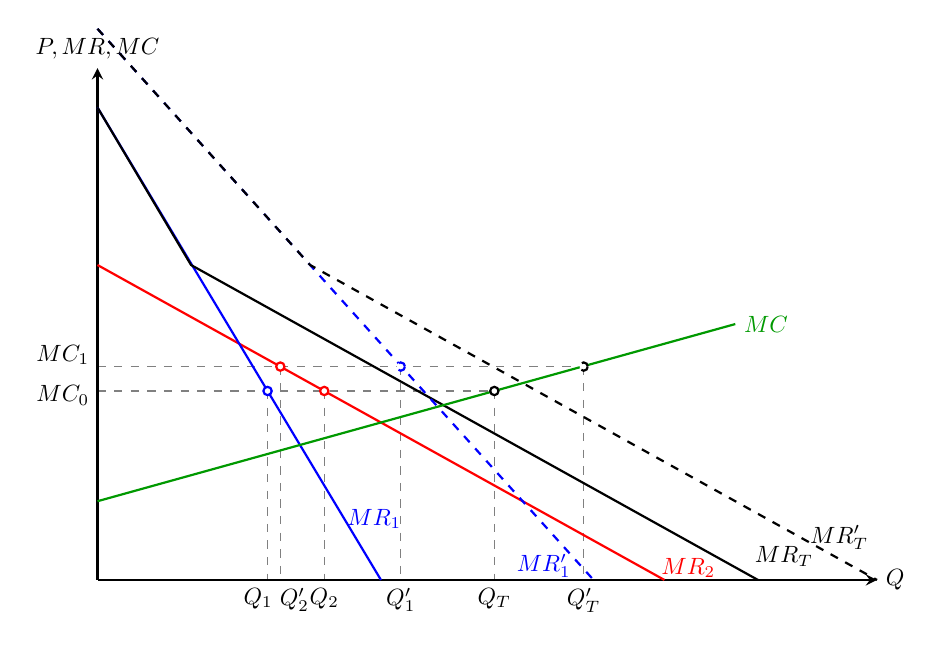
\begin{tikzpicture}[x=1.8cm, y=1.0cm, >=stealth, thick, every node/.style={scale=0.85}]
				% 2. 辅助虚线与防重叠标签 (底层)
				% 初始状态 (MC_0 = 2.4)
				\draw[dashed, thin, gray] (0, 2.4) node[left, text=black, yshift=-2pt] {$MC_0$} -- (2.8, 2.4);
				\draw[dashed, thin, gray] (1.2, 2.4) -- (1.2, 0) node[below, text=black, xshift=-4pt] {$Q_1$};
				\draw[dashed, thin, gray] (1.6, 2.4) -- (1.6, 0) node[below, text=black] {$Q_2$};
				\draw[dashed, thin, gray] (2.8, 2.4) -- (2.8, 0) node[below, text=black] {$Q_T$};
				
				% 变动后状态 (MC_1 = 2.71)
				\draw[dashed, thin, gray] (0, 2.71) node[left, text=black, yshift=5pt] {$MC_1$} -- (3.43, 2.71);
				\draw[dashed, thin, gray] (2.14, 2.71) -- (2.14, 0) node[below, text=black] {$Q_1'$};
				% Q_2' (1.29) 与 Q_1 (1.2) 在横轴上距离过近，采用物理分离（高度错落排版）彻底防重叠
				\draw[dashed, thin, gray] (1.29, 2.71) -- (1.29, 0) node[below, text=black, xshift=6pt] {$Q_2'$};
				\draw[dashed, thin, gray] (3.43, 2.71) -- (3.43, 0) node[below, text=black] {$Q_T'$};
				
				% 3. 坐标轴
				\draw[->] (0,0) -- (5.5,0) node[right] {$Q$};
				\draw[->] (0,0) -- (0,6.5) node[above] {$P, MR, MC$};
				
				% 4. 绘图代码
				% 市场 2 的 MR (保持不变)
				\draw[domain=0:4, color=red] plot (\x, {4 - \x}) node[right,yshift=5pt,xshift=-5pt] {$MR_2$};
				% 市场 1 的初始 MR
				\draw[domain=0:2, color=blue] plot (\x, {6 - 3*\x}) node[right,xshift=-18pt,yshift=26pt] {$MR_1$};
				% 总的初始 MR_T (分段)
				\draw[color=black] (0, 6) -- (0.66, 4) -- (4.66, 0);
				\node[black, right,xshift=-5pt] at (4.66, 0.3) {$MR_T$};
				
				% 市场 1 变动后的 MR_1'
				\draw[domain=0:3.5, color=blue, dashed] plot (\x, {7 - 2*\x}) node[left,yshift=6pt,xshift=-6pt] {$MR_1'$};
				% 总的变动后 MR_T' (分段)
				\draw[color=black, dashed] (0, 7) -- (1.5, 4) -- (5.5, 0);
				\node[black, left,yshift=8pt] at (5.5, 0.3) {$MR_T'$};
				
				% 边际成本 MC
				\draw[domain=0:4.5, color=green!60!black] plot (\x, {0.5*\x + 1}) node[right] {$MC$};
				
				% 5. 均衡点标号
				\fill[white] (1.2, 2.4) circle (1.5pt); \draw[blue] (1.2, 2.4) circle (1.5pt);
				\fill[white] (1.6, 2.4) circle (1.5pt); \draw[red] (1.6, 2.4) circle (1.5pt);
				\fill[white] (2.8, 2.4) circle (1.5pt); \draw[black] (2.8, 2.4) circle (1.5pt);
				
				\fill[white] (2.14, 2.71) circle (1.5pt); \draw[blue, dashed] (2.14, 2.71) circle (1.5pt);
				\fill[white] (1.29, 2.71) circle (1.5pt); \draw[red] (1.29, 2.71) circle (1.5pt);
				\fill[white] (3.43, 2.71) circle (1.5pt); \draw[black, dashed] (3.43, 2.71) circle (1.5pt);
			\end{tikzpicture}
		\end{center}
		\newpage
		
		\item \textbf{在对批发给经销商的汽车定价时，美国的汽车公司典型地对“豪华配置”（例如真皮座椅等）的成本的百分比加价比对汽车本身或对较“基本”配置（如动力方向盘和自动变速器）的加成要高得多。解释原因？}
		
		\textbf{答：}
		这是一种基于产品特征进行甄别的典型三级价格歧视策略。汽车公司通过提供不同档次的配置，将潜在消费者自发地划分为对价格极为敏感的群体和对价格不敏感的群体，并以此实施差异化的加成定价。
		
		购买汽车基础配置的消费者通常面临较硬的预算约束，将汽车视为代步工具，其对应的需求价格弹性较高。相反，愿意支付额外费用选装真皮座椅或高级音响等豪华配置的消费者，通常具有更高的收入水平和强烈的享受型消费动机。这部分群体对价格变动的敏感度极低，表现出显著较低的需求价格弹性。
		
		根据利润最大化的逆弹性定价法则，价格加成幅度与需求价格弹性的绝对值成反比：
		\[
		\begin{aligned}
			\frac{P - MC}{P} = -\frac{1}{E_d}
		\end{aligned}
		\]
		
		该法则表明，目标群体的需求弹性绝对值越小，厂商能够并且应当设定的利润加成百分比就越高。因此，汽车厂商对需求缺乏弹性的“豪华配置”设定了远高于“基础配置”的成本加成，以此在不流失基础盘销量的前提下，精准且最大化地榨取高收入群体的消费者剩余。
		
		\item \textbf{为什么高峰负荷定价是价格歧视的一种形式？它能使消费者受益吗？举一个例子。}
		
		\textbf{答：}
		高峰负荷定价在表象上类似于三级价格歧视，因其针对同一商品在不同时段向消费者索取不同价格。然而，从严格的微观经济学定价机制来看，两者存在本质区别。
		
		价格歧视的核心前提是服务不同群体的边际成本相同，厂商仅依靠需求价格弹性的差异来进行差别定价；而在高峰负荷定价中，由于厂商在需求高峰期面临刚性的产能限制，导致该时段的边际成本急剧攀升，各时期的价格差异实际上是对独立且真实变动的边际成本的反映。
		
		\begin{center}
			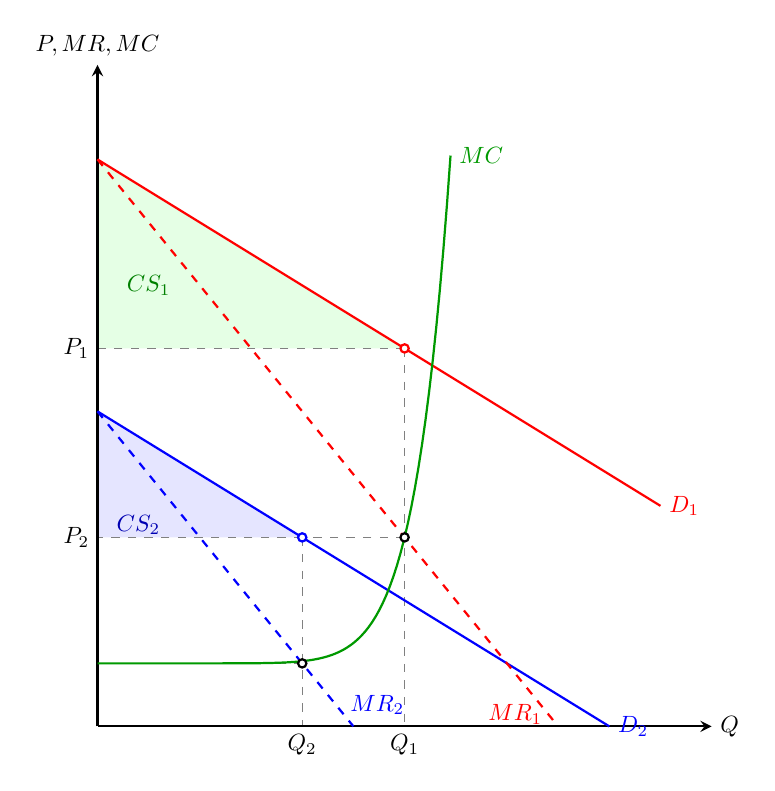
\begin{tikzpicture}[x=1.3cm, y=0.8cm, >=stealth, thick, every node/.style={scale=0.85}]
				% 1. 福利或剩余区域填充 (最底层)
				% 高峰期 CS (CS1)
				\fill[green!10] (0, 9) -- (0, 6) -- (3, 6) -- cycle;
				\node[green!50!black] at (0.5, 7) {$CS_1$};
				
				% 非高峰期 CS (CS2)
				\fill[blue!10] (0, 5) -- (0, 3) -- (2, 3) -- cycle;
				\node[blue!70!black] at (0.4, 3.2) {$CS_2$};
				
				% 2. 辅助虚线与防重叠标签
				\draw[dashed, thin, gray] (2, 3) -- (2, 0) node[below, text=black] {$Q_2$};
				\draw[dashed, thin, gray] (2, 3) -- (0, 3) node[left, text=black] {$P_2$};
				
				\draw[dashed, thin, gray] (3, 6) -- (3, 0) node[below, text=black] {$Q_1$};
				\draw[dashed, thin, gray] (3, 6) -- (0, 6) node[left, text=black] {$P_1$};
				
				% 均衡交点到轴的连线 (MR=MC点)
				\draw[dashed, thin, gray] (2, 1) -- (0, 1);
				\draw[dashed, thin, gray] (3, 3) -- (2, 3); 
				
				% 3. 坐标轴
				\draw[->] (0,0) -- (6,0) node[right] {$Q$};
				\draw[->] (0,0) -- (0,10.5) node[above] {$P, MR, MC$};
				
				% 4. 绘图代码
				% 非高峰期需求与边际收益
				\draw[domain=0:5, color=blue] plot (\x, {5 - \x}) node[right] {$D_2$};
				\draw[domain=0:2.5, color=blue, dashed] plot (\x, {5 - 2*\x}) node[right, yshift=9pt,xshift=-5pt] {$MR_2$};
				
				% 高峰期需求与边际收益
				\draw[domain=0:5.5, color=red] plot (\x, {9 - \x}) node[right] {$D_1$};
				\draw[domain=0:4.5, color=red, dashed] plot (\x, {9 - 2*\x}) node[left,yshift=5pt,xshift=-3pt] {$MR_1$};
				
				% 边际成本 MC (平缓后急剧上升，模拟产能约束)
				\draw[domain=0:3.45, color=green!60!black, samples=100] plot (\x, {1 + 2*(\x/3)^10}) node[right] {$MC$};
				
				% 5. 均衡点与标号 (fill=white清除交叉线)
				% 需求曲线上的定价点
				\fill[white] (2, 3) circle (1.5pt); \draw[blue] (2, 3) circle (1.5pt);
				\fill[white] (3, 6) circle (1.5pt); \draw[red] (3, 6) circle (1.5pt);
				
				% MR=MC 的利润最大化产量决定点
				\fill[white] (2, 1) circle (1.5pt); \draw[black] (2, 1) circle (1.5pt);
				\fill[white] (3, 3) circle (1.5pt); \draw[black] (3, 3) circle (1.5pt);
			\end{tikzpicture}
		\end{center}
		实行该定价策略通过消除单一价格下的市场扭曲，实质性地改善了消费者福利乃至社会总福利。如果公共设施强制设定统一的平均价格，会导致高峰期出现严重的过度需求与短缺，而非高峰期则产生大量的产能闲置。
		
		如图所示，厂商面临非高峰期需求 $D_2$ 与高峰期需求 $D_1$。在非高峰期，资源未达到产能瓶颈，边际成本极低且平缓，厂商根据 $MR_2 = MC$ 的利润最大化原则设定较低的价格 $P_2$ 与产量 $Q_2$；而在高峰期，由于逼近产能极限，边际成本高昂且陡峭，厂商根据 $MR_1 = MC$ 设定较高的价格 $P_1$ 与产量 $Q_1$。这种紧随边际成本波动的动态定价不仅实现了资源的帕累托最优配置，还使得那些对价格敏感的消费者能够在非高峰期以极低的 $P_2$ 进入市场，从而获得了图中标注为 $CS_2$ 的新增消费者剩余，极大地增加了这一特定群体的福利总额（电影院按日场和夜场成本独立定价便属于此类典型机制）。
		
		
		
		\item \textbf{如果某厂商有两个具有不同需求曲线的顾客，它怎样确定一种最优的两部收费？（假设它了解顾客的需求曲线。）}
		
		\textbf{答：}
		当厂商面临具有不同需求规模的异质性消费者时，单一两部收费（收取固定的入门费 $T$ 和单位使用费 $P$）的定价决策需要权衡消费者剩余的榨取与总使用利润的获取。如果厂商试图将使用费定为等于边际成本（$P=MC$），为了不失去低需求消费者，它只能将入门费 $T$ 设定为该消费者在边际成本价格下所能获得的全部剩余。这虽然保证了销量，但未能从高需求消费者那里榨取充分的利润。
		
		为了实现全局利润最大化，厂商应当将使用费提高至边际成本之上（$P^* > MC$），并同步将入门费设定为在新的较高使用费下，低需求消费者所剩余的全部消费者剩余。
		
		如图所示，这种策略虽然损失了部分由低需求者贡献的入门费，但通过对所有消耗的产品收取高于边际成本的使用费，获得了更为可观的补偿。已知低需求曲线 $D_1$ 和高需求曲线 $D_2$，厂商的总利润函数可表示为入门费与两市场总销量的函数：
		\[
		\begin{aligned}
			\pi = 2T^* + (P^* - MC)(Q_1 + Q_2)
		\end{aligned}
		\]
		
		厂商通过微积分最优化技术求解该函数，即可确定具体的 $P^*$ 和 $T^*$。在该均衡状态下，由于对高需求消费者征收了大量可变利润，厂商获得的最大化总利润必然大于单纯定价在边际成本时截取的两倍低需求者剩余面积。
		
		\begin{center}
			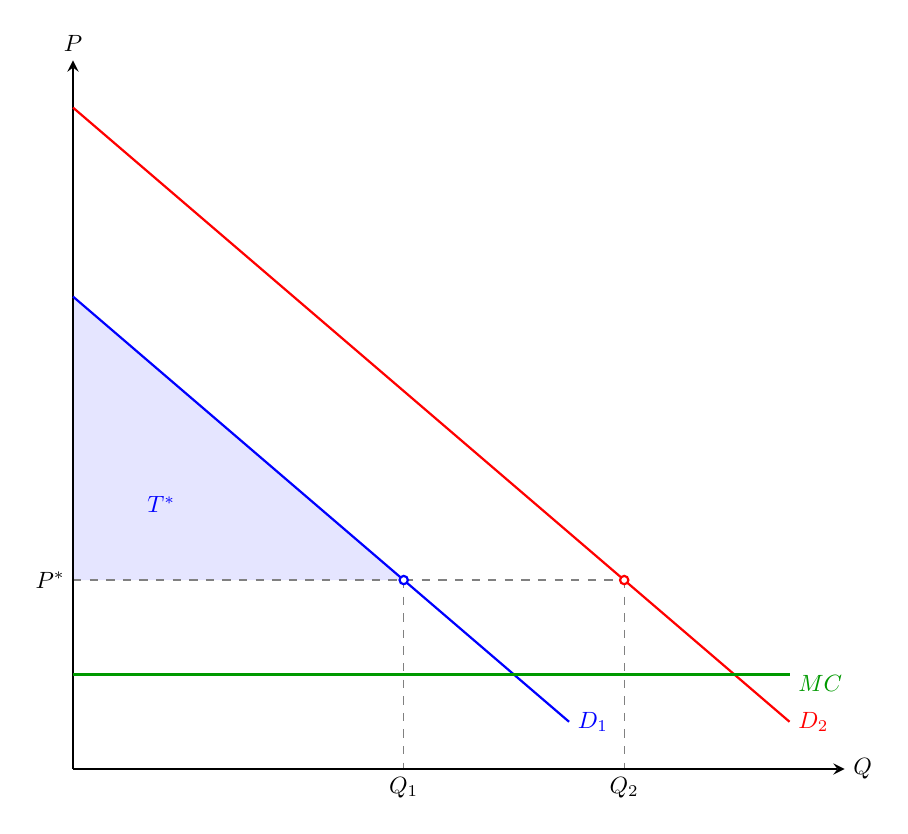
\begin{tikzpicture}[x=1.4cm, y=1.2cm, >=stealth, thick, every node/.style={scale=0.85}]
				% 1. 福利或剩余区域填充 (最底层)
				\fill[blue!10] (0, 5) -- (0, 2) -- (3, 2) -- cycle;
				\node[blue] at (0.8, 2.8) {$T^*$};
				
				% 2. 辅助虚线与防重叠标签
				\draw[dashed, thin, gray] (3, 2) -- (3, 0) node[below, text=black] {$Q_1$};
				\draw[dashed, thin, gray] (5, 2) -- (5, 0) node[below, text=black] {$Q_2$};
				\draw[dashed, thin, gray] (0, 2) node[left, text=black] {$P^*$} -- (5, 2);
				
				% 3. 坐标轴
				\draw[->] (0,0) -- (7,0) node[right] {$Q$};
				\draw[->] (0,0) -- (0,7.5) node[above] {$P$};
				
				% 4. 绘图代码
				\draw[domain=0:4.5, color=blue] plot (\x, {5 - \x}) node[right] {$D_1$};
				\draw[domain=0:6.5, color=red] plot (\x, {7 - \x}) node[right] {$D_2$};
				\draw[domain=0:6.5, color=green!60!black] plot (\x, {1}) node[right, yshift=-4pt] {$MC$};
				
				% 5. 均衡点与标号 (fill=white)
				\fill[white] (3, 2) circle (1.5pt); \draw[blue] (3, 2) circle (1.5pt);
				\fill[white] (5, 2) circle (1.5pt); \draw[red] (5, 2) circle (1.5pt);
			\end{tikzpicture}
		\end{center}
		
		\item \textbf{为什么吉列安全剃须刀的定价是一种两部收费？吉列必须是它的刀片以及它的剃须刀的垄断生产者吗？假设吉列正在向你咨询如何决定两部收费，你会建议怎样做？}
		
		\textbf{答：}
		吉列安全剃须刀的商业模式是经济学中经典的互补品两部收费策略的体现。消费者必须先购买剃须刀架这一固定资产，这构成了准入市场所需支付的固定“入门费”（$T$）；随后持续消耗的替换刀片，则构成了与其使用频率直接相关的“使用费”（$P$）。
		
		吉列并不一定要是绝对的垄断生产者，但必须在互补品组件上拥有显著的市场势力。厂商必须通过技术专利保护、特有接口设计或系统封闭性来实现产品物理上的硬捆绑。只有防止竞争对手在市场上供应通用兼容且价格低廉的替换刀片，吉列才能在维持使用费高于边际成本的同时，迫使消费者在封闭生态内支付入门费并接受两部收费机制。
		
		在制定具体的两部收费战略时，厂商必须深入评估目标消费群体的需求异质性。当目标市场的需求规模高度同质化时，厂商应将刀片使用费定为等于或极接近边际成本（$P=MC$），同步设定高昂的剃须刀架入门费，以此一次性、无损地榨取所有消费者的消费者剩余。
		
		当市场存在显著的低频与高频异质性需求时，过高的刀架价格将直接把低频消费者排斥在市场之外。此时，厂商应当大幅降低甚至以低于成本的价格销售剃须刀架（$T$）以扩大用户基数，并将刀片使用费大幅定在边际成本之上（$P>MC$）。通过这种方式，厂商依靠高频剃须群体对高利润刀片的持续消耗来弥补硬件亏损，并实现长期总利润的最大化。
		
		\item \textbf{在加利福尼亚州伍德兰小镇，有许多牙医但只有一个眼科医生。对于牙齿检查或眼睛检查，哪个项目有钱人将更可能被提供折扣价格？为什么？}
		
		\textbf{答：}
		对于这两项检查，有钱人不仅不会获得折扣，反而更有可能在眼科检查中被定向索取高价。
		
		在完全竞争的牙医市场中，由于存在大量替代供给，厂商完全不具备市场势力，无法实施任何形式的价格歧视。此时市场统一价格被竞争机制推平至等于边际成本：
		\[
		\begin{aligned}
			P = MC
		\end{aligned}
		\]
		在这种市场结构下，不论患者的收入高低，任何牙医都无法提供低于成本的折扣。
		
		相反，作为当地唯一供给者的眼科医生拥有绝对的垄断势力，具备实施三级价格歧视的基础条件。根据逆弹性定价法则，垄断者制定差异化价格的依据是不同群体的需求价格弹性：
		\[
		\begin{aligned}
			\frac{P - MC}{P} = -\frac{1}{E_d}
		\end{aligned}
		\]
		相较于低收入群体，有钱人通常面临极高的搜寻成本和时间成本，且对医疗费用的变动极不敏感，这导致其呈现出极低的需求价格弹性。为了实现总利润的最大化，眼科医生必然会对高弹性的低收入群体提供折扣以保住市场份额，同时对低弹性的有钱人群体实施价格歧视，索取最高水平的单价。
		
		\item \textbf{为什么 MGM 要将《飘》和《吉蒂的奖赏》捆绑销售？若捆绑销售能增加利润，需求必须具备什么特征？}
		
		\textbf{答：}
		MGM 采用纯捆绑销售策略的核心目的在于通过平抑异质性需求来攫取原本散落的消费者剩余。假设采取分别销售模式，为了不流失任何一家影院的订单，《飘》的单价上限只能定为 $10000$ 美元，《吉蒂的奖赏》的单价上限只能定为 $3000$ 美元。在此策略下，总收益被死死限制在较低水平：
		\[
		\begin{aligned}
			TR_{\text{分别销售}} = 10000 \times 2 + 3000 \times 2 = 26000
		\end{aligned}
		\]
		
		若实施捆绑销售，影院 A 对两部电影的总估值为 $15000$ 美元，影院 B 为 $14000$ 美元。厂商以组合估值下限 $14000$ 美元作为统一定价，依然可以同时卖给两家影院，此时总收益大幅跃升：
		\[
		\begin{aligned}
			TR_{\text{捆绑销售}} = 14000 \times 2 = 28000
		\end{aligned}
		\]
		
		\begin{center}
			\begin{tabular}{lcc}
				\hline
				& 《飘》保留价格 & 《吉蒂的奖赏》保留价格 \\
				\hline
				影院 A & $12000$ 美元 & $3000$ 美元 \\
				影院 B & $10000$ 美元 & $4000$ 美元 \\
				\hline
			\end{tabular}
		\end{center}
		
		捆绑销售若要实现利润增值，核心前提是消费者对不同商品的保留价格必须呈现负相关特征。即愿意为某部特定影片支付高价的消费者，必须对应只愿为另一部影片支付较低的价格。
		
		若需求呈现严格的正相关，即某消费者对所有商品的估值均单边碾压另一消费者，如以下表格所示。影院 A 对两部电影的总估值（$16000$ 美元）全面高于影院 B（$13000$ 美元）。若此时实施捆绑销售，为了促成全市场交易，捆绑价只能被迫降至 $13000$ 美元。最终总收入为 $26000$ 美元，与分别销售时的利润毫无二致，捆绑策略彻底失效。
		
		\begin{center}
			\begin{tabular}{lcc}
				\hline
				& 《飘》保留价格 & 《吉蒂的奖赏》保留价格 \\
				\hline
				影院 A & $12000$ 美元 & $4000$ 美元 \\
				影院 B & $10000$ 美元 & $3000$ 美元 \\
				\hline
			\end{tabular}
		\end{center}
		
		\item \textbf{混合捆绑销售与纯捆绑销售有何不同？在什么条件下混合捆绑销售优于纯捆绑销售？为什么许多餐馆实行混合捆绑销售（通过供应套餐和点菜）而不是纯捆绑销售？}
		
		\textbf{答：}
		纯捆绑销售是一种极其刚性的定价策略，它剥夺了消费者的拆分购买权，要求其只能完整购买一揽子商品组合。混合捆绑销售则赋予了消费者自主选择的机制，允许其以略低于单品总价的组合优惠价购买全套产品，或者按相对高昂的单价独立购买部分组件。
		
		当市场满足两个核心微观条件时，混合捆绑销售的利润转化边界将绝对超越纯捆绑销售。一方面，消费者需求不能是完美的负相关，必须存在极大的估值离散度；另一方面，商品本身必须具备不可忽视的边际生产成本。在纯捆绑模式下，厂商往往会强迫某些对特定单品估值极低（甚至低于边际成本）的消费者购买该组件，这不仅造成了生产资源的无谓消耗，还倒逼厂商必须拉低整体捆绑包的定价上限。
		
		许多餐馆采用混合捆绑（即同时提供折扣套餐与高价单点）正是受制于极具差异化的消费者偏好与食材真实的边际成本约束。
		
		部分顾客对主菜和餐后甜点均有均衡且极高的评价，这部分人群构成套餐的完美受众群体。然而，另一部分顾客受限于预算或饮食习惯，仅对主菜有极高的支付意愿，对甜点的估值甚至远远低于厨房制作该甜点的边际成本。
		
		如果强制推行纯捆绑，餐馆要么彻底流失这部分偏好单一的顾客，要么在他们身上被动承受甜点高昂边际成本的绝对亏损。通过引入混合捆绑机制，餐馆用高溢价的单点菜单彻底榨取了偏好单一者的消费者剩余，同时用折扣套餐锁定了偏好均衡者的整体利润，完美规避了边际成本倒挂的风险并实现了跨客群的最优提取。
		
		\item \textbf{搭售与捆绑销售有何不同？为什么厂商想要实行搭售？}
		
		\textbf{答：}
		搭售通常涉及具有严格互补关系的主产品与消耗品，其核心机制在于强迫购买，即消费者在购买某一产品时必须连带购买另一特定产品。捆绑销售的适用范围更为广泛，组合内的商品既可以是互补品，也可以是独立的替代品，且往往允许消费者进行混合选择。厂商实施搭售策略的根本动机是将其作为一种计量潜在需求的甄别工具，以克服信息不对称并实现近似的完全价格歧视。在经典的 IBM 穿孔卡片案例中，厂商以接近甚至低于成本的低价出租大型计算机主机（主产品），但强制要求客户必须配套使用其垄断生产的高价穿孔卡片（搭售品）。高频使用计算机的大规模企业必然消耗海量卡片，从而被厂商精准识别并以高额的卡片溢价榨取了其巨大的消费者剩余，这使得搭售成为在异质性需求市场中最大化厂商总利润的有效手段。
		
		\item \textbf{为什么广告投入增加到最后 1 美元广告支出正好产生 1 美元额外销售这一点是不正确的？什么是边际广告费的正确法则？}
		
		\textbf{答：}
		这割裂了销售与生产的内在物理联系，其核心谬误在于完全忽略了满足新增需求所必须付出的边际生产成本（$MC$）。
		
		如图所示，假设厂商初始处于未投放广告的均衡状态，面临需求曲线 $D_0$ 与边际收益曲线 $MR_0$，利润最大化产量为 $Q_0$。当厂商增加广告支出时，成功将需求曲线向右推移至 $D_1$（对应的边际收益移至 $MR_1$）。此时，厂商为了在新的交点实现利润最大化，必须将产量扩张至 $Q_1$。这一产量的扩张并非无代价的，它迫使厂商沿着向上倾斜的边际成本曲线（$MC$）移动，图中标注的阴影区域即为必须额外支付的实际生产成本。
		
		因此，增加一单位广告支出，厂商不仅要承担广告本身的绝对成本（$1$ 美元），还要承担由新增销量 $\Delta Q$ 所引发的额外生产成本。正确的边际广告费法则要求广告投放推进至其带来的边际收益恰好等于总的边际成本之和。若 $\Delta A$ 代表增加的广告支出，该均衡条件可表达为：
		\[
		\begin{aligned}
			P \frac{\Delta Q}{\Delta A} = 1 + MC \frac{\Delta Q}{\Delta A}
		\end{aligned}
		\]
		为了便于企业在实际经营中进行统筹决策，通过代数重排与弹性代换，该法则可转化为基于弹性指标的直观等式：
		\[
		\begin{aligned}
			\frac{A}{PQ} = -\frac{E_A}{E_D}
		\end{aligned}
		\]
		
		\begin{center}
			\begin{tikzpicture}[x=1.2cm, y=0.8cm, >=stealth, thick, every node/.style={scale=0.85}]
				% 1. 福利或剩余区域填充 (最底层)
				% 填充新增的生产成本区域 (沿着 MC 曲线从 Q0 到 Q1 的下方梯形面积)
				\fill[red!10] (2, 0) -- (2, 2) -- (3.2, 2.6) -- (3.2, 0) -- cycle;
				\node[red!60!black] at (2.6, 0.5) {新增生产成本};
				
				% 2. 辅助虚线与防重叠标签
				% 初始均衡辅助线
				\draw[dashed, thin, gray] (2, 4) -- (2, 0) node[below, text=black] {$Q_0$};
				\draw[dashed, thin, gray] (2, 4) -- (0, 4) node[left, text=black] {$P_0$};
				\draw[dashed, thin, gray] (2, 2) -- (0, 2); 
				
				% 广告后均衡辅助线
				\draw[dashed, thin, gray] (3.2, 5.8) -- (3.2, 0) node[below, text=black] {$Q_1$};
				\draw[dashed, thin, gray] (3.2, 5.8) -- (0, 5.8) node[left, text=black] {$P_1$};
				\draw[dashed, thin, gray] (3.2, 2.6) -- (0, 2.6);
				
				% 3. 坐标轴
				\draw[->] (0,0) -- (6,0) node[right] {$Q$};
				\draw[->] (0,0) -- (0,9) node[above] {$P, MR, MC$};
				
				% 4. 绘图代码
				% 初始需求与边际收益
				\draw[domain=0:4.5, color=blue] plot (\x, {6 - \x}) node[above] {$D_0$};
				\draw[domain=0:2.5, color=blue, dashed] plot (\x, {6 - 2*\x}) node[right] {$MR_0$};
				
				% 广告后需求与边际收益
				\draw[domain=0:5.5, color=red] plot (\x, {9 - \x}) node[above] {$D_1$};
				\draw[domain=0:4, color=red, dashed] plot (\x, {9 - 2*\x}) node[right] {$MR_1$};
				
				% 边际成本 MC
				\draw[domain=0:5, color=green!60!black] plot (\x, {1 + 0.5*\x}) node[left,yshift=3pt] {$MC$};
				
				% 5. 均衡点与标号 (fill=white清除交叉线)
				\fill[white] (2, 4) circle (1.5pt); \draw[blue] (2, 4) circle (1.5pt);
				\fill[white] (2, 2) circle (1.5pt); \draw[black] (2, 2) circle (1.5pt);
				
				\fill[white] (3.2, 5.8) circle (1.5pt); \draw[red] (3.2, 5.8) circle (1.5pt);
				\fill[white] (3.2, 2.6) circle (1.5pt); \draw[black] (3.2, 2.6) circle (1.5pt);
				
				% 箭头指示需求推移
				\draw[->, very thick, gray] (4.6, 1.4) -- (5.6, 3.4);
			\end{tikzpicture}
		\end{center}
		\newpage
		\item \textbf{厂商如何检查它的广告对销售比率是否合理？它需要什么信息？}
		
		\textbf{答：}
		厂商可以依据利润最大化条件推导出的广告经验法则，从数学上来精准评估其当前的广告与销售比率是否处于最优边界。根据边际收益等于边际成本的均衡法则，最优的广告支出占比可被分解如下：
		\[
		\begin{aligned}
			\frac{P - MC}{P} \times \left( \frac{A}{Q} \times \frac{\Delta Q}{\Delta A} \right) = \frac{A}{PQ}
		\end{aligned}
		\]
		等式左侧括号内的乘积项在经济学上定义为广告的需求弹性（$E_A$），即广告支出每变动百分之一所引起的需求量变动的百分比。同时，根据基于垄断势力定价的勒纳指数公式，价格加成率 $\frac{P - MC}{P}$ 在最优均衡下严格等于 $-\frac{1}{E_D}$。将这两项代入替换后，厂商理论上的最优广告对销售比率必须等于负的广告需求弹性与产品价格弹性之比：
		\[
		\begin{aligned}
			\frac{A}{PQ} = -\frac{E_A}{E_D}
		\end{aligned}
		\]
		为了应用该数学法则进行实证检验，厂商必须通过市场调研与计量经济学工具获取两项核心的参数信息：目标市场的价格需求弹性（$E_D$）以及消费者对广告变动的敏感度（$E_A$）。厂商只需将这两个估测出的弹性参数代入上述公式，计算出理论上的最优比值，并将其与财务报表中的实际广告营收比进行对比。若实际比值低于理论值，说明边际广告收益仍大于成本，厂商应继续扩张广告预算；若实际比值偏高，则表明广告支出已陷入边际效用递减阶段，应当立即缩减营销开支。
		
		\newpage
	\end{enumerate}
	\section{练习题}
	\begin{enumerate}[label=\textbf{\arabic*.}, leftmargin=*]
		\item \textbf{价格歧视需要有将顾客分类的能力和防止套利的能力。解释下列项目是怎样起价格歧视的作用的，并讨论其分类和套利。}
		
		\textbf{答：}
		针对要求周末在家过夜的特价机票，航空公司通过这一时间限制条件将旅客精准划分为对价格不敏感的商务旅客和对价格高度敏感的休闲旅游者。由于机票采用实名登记与身份核验机制，这种物理层面的严格管控彻底封死了低价票向高价群体倒卖的套利空间。
		
		针对以购买者住址为定价基础的水泥送货服务，厂商实质上实施了空间价格歧视，将运费差异内化于最终报价中以实现按地理位置的客群分割。由于水泥具有极大的体积与重量，其高昂的二次物流运输成本远远超过了潜在的套利价差，从而在物理形态上阻断了跨区域套利行为。
		
		针对销售食品加工机时附送的回扣优惠券，厂商利用消费者对兑换时间与精力成本的敏感度，将顾客自动甄别为高机会成本（低价格弹性）与低机会成本（高价格弹性）两个独立群体。为了防止套利，厂商通常通过限制单个家庭住址的兑换总数或绑定机器唯一的硬件序列号来维持市场的严格分割。
		
		针对卫生纸提供的临时促销活动属于典型的跨期价格歧视策略。厂商利用不同消费者对商品库存的容忍度进行分类，价格敏感型消费者会在促销期大量囤货，而缺乏耐心的不敏感型消费者只按需高价购买。尽管实物商品存在转售可能，但卫生纸单位价值极低且占据庞大仓储空间，其储存与转卖的交易成本足以彻底抹平套利利润。
		
		针对整形外科医生向高收入病人索取更高费用的行为，医生在术前面诊过程中通过观察和交流探查病人的支付意愿与收入水平，从而实现个体的精准甄别。由于医疗服务直接作用于患者本人的身体，具备绝对的非排他性和不可转让性，低价购买的“手术服务”绝无可能被剥离并转售给高收入群体，套利在逻辑层面上被完全杜绝。
		
		\item \textbf{如果夫妻对汽车影院的需求比单身个人更有弹性，则影院向开车者收门票费并向乘车者收额外的费用是最优的。这种说法对还是错？试解释。}
		
		\textbf{答：}
		正确。这种定价模式本质上是针对具有异质性需求的群体所实施的互补性两部收费策略。
		
		\begin{center}
			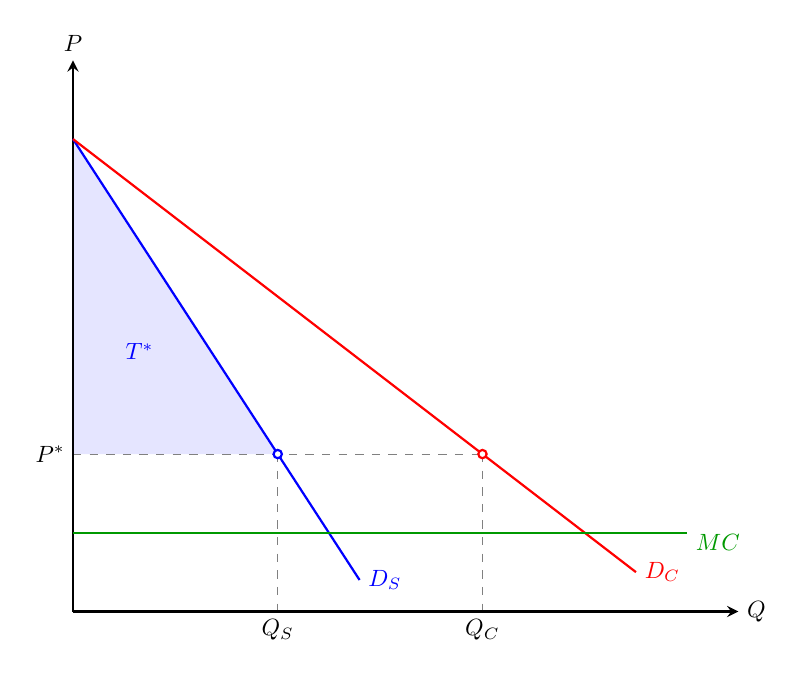
\begin{tikzpicture}[x=1.3cm, y=1.0cm, >=stealth, thick, every node/.style={scale=0.85}]
				% 1. 福利或剩余区域填充 (最底层)
				% 入门费 T* (等于单身群体的 CS)
				\fill[blue!10] (0, 6) -- (0, 2) -- (2, 2) -- cycle;
				\node[blue] at (0.65, 3.3) {$T^*$};
				
				% 2. 辅助虚线与防重叠标签
				\draw[dashed, thin, gray] (2, 2) -- (2, 0) node[below, text=black] {$Q_S$};
				\draw[dashed, thin, gray] (4, 2) -- (4, 0) node[below, text=black] {$Q_C$};
				\draw[dashed, thin, gray] (0, 2) node[left, text=black] {$P^*$} -- (4, 2);
				
				% 3. 坐标轴
				\draw[->] (0,0) -- (6.5,0) node[right] {$Q$};
				\draw[->] (0,0) -- (0,7) node[above] {$P$};
				
				% 4. 绘图代码
				% 单身需求 (缺乏弹性，较陡峭)
				\draw[domain=0:2.8, color=blue] plot (\x, {6 - 2*\x}) node[right] {$D_S$};
				% 夫妻需求 (富有弹性，较平缓)
				\draw[domain=0:5.5, color=red] plot (\x, {6 - \x}) node[right] {$D_C$};
				% 边际成本 MC
				\draw[domain=0:6, color=green!60!black] plot (\x, {1}) node[right, yshift=-4pt] {$MC$};
				
				% 5. 均衡点与标号 (fill=white清除交叉线)
				\fill[white] (2, 2) circle (1.5pt); \draw[blue] (2, 2) circle (1.5pt);
				\fill[white] (4, 2) circle (1.5pt); \draw[red] (4, 2) circle (1.5pt);
			\end{tikzpicture}
		\end{center}
		
		汽车影院向开车者收取的固定门票费构成了准入市场的“入门费”（$T$），而向乘车者收取的额外费用则构成了边际“使用费”（$P$）。由于单身个人独自承担高昂的入门费，其人均观影成本必然高于两人共同分摊入门费与边际使用费的夫妻群体。这种价格结构的内在机制完美契合了目标市场的弹性特征。夫妻群体由于面临更多的替代娱乐选择或受制于家庭预算约束，呈现出较高的需求价格弹性，厂商必须为其提供较低的人均实际价格以促成交易；相反，单身个人具有更低的价格弹性，厂商可以通过向其榨取全额入门费来最大化获取利润。
		
		如图所示，我们可以将这一微观定价逻辑映射至标准的异质性需求两部收费模型中。厂商面临缺乏弹性的单身群体需求 $D_S$ 与富有弹性的夫妻群体需求 $D_C$。为了实现全局利润最大化，厂商不会将使用费设定为等于边际成本（$MC$），而是将其战略性地提升至 $P^*$。同时，厂商将入门费 $T^*$ 严格设定为在该价格下单身群体（即需求较弱者）所能获得的全部消费者剩余（图中标注的蓝色阴影面积）。
		
		在这个最优化均衡中，厂商牺牲了少部分单身人群的固定的入门费空间，却成功地以高于边际成本的使用费 $P^*$ 从弹性大、人数多（或消费频次高）的夫妻群体身上攫取了更为可观的增量利润，最终实现总利润越过单一统一定价的边界。
		
		
		
		\item \textbf{在教材例 11.1 中，加工食品及相关消费品的制造商使用优惠券作为价格歧视的一种方式。尽管优惠券在美国很盛行，在其他一些国家情况却不同。例如在德国，优惠券是非法行为。（1）禁止在德国使用优惠券是改善了还是恶化了德国消费者的境况？（2）禁止在德国使用优惠券是改善了还是恶化了德国生产者的境况？}
		
		\textbf{答：}
		禁止使用优惠券对消费者总境况的影响在理论上是不确定的，但在很大程度上极有可能恶化了消费者的整体福利水平。优惠券作为实施三级价格歧视的工具，其对消费者剩余的最终净影响取决于市场的扩张效应。
		
		\begin{center}
			\begin{tikzpicture}[x=0.7cm, y=0.7cm, >=stealth, thick, every node/.style={scale=0.85}]
				% ==== 左侧：第1组消费者 (高WTP) ====
				\begin{scope}
					% 福利填充
					\fill[green!15] (0, 8) -- (0, 4) -- (4, 4) -- cycle;
					\node[green!50!black] at (1.0, 5.0) {$CS_1$};
					
					% 辅助线
					\draw[dashed, thin, gray] (4, 4) -- (4, 0) node[below, text=black] {$Q_1$};
					\draw[dashed, thin, gray] (4, 4) -- (0, 4) node[left, text=black] {$P_1 = P_U$};
					
					% 坐标轴
					\draw[->] (0,0) -- (6,0) node[right] {$Q$};
					\draw[->] (0,0) -- (0,9) node[above] {$P$};
					
					% 绘图代码
					\draw[domain=0:6, color=blue] plot (\x, {8 - \x}) node[right] {$D_1$};
					\draw[domain=0:3.5, color=blue, dashed] plot (\x, {8 - 2*\x}) node[below] {$MR_1$};
					\draw[domain=0:6, color=green!60!black] plot (\x, {0}) node[below, yshift=-5pt] {$MC=0$};
					
					% 标号
					\fill[white] (4, 4) circle (1.5pt); \draw[black] (4, 4) circle (1.5pt);
					\node at (3, 8.5) {\textbf{第 1 组（不敏感市场）}};
				\end{scope}
				
				% ==== 右侧：第2组消费者 (低WTP) ====
				\begin{scope}[xshift=8cm]
					% 福利填充
					\fill[orange!15] (0, 3) -- (0, 1.5) -- (1.5, 1.5) -- cycle;
					\node[orange!60!black] at (1, 2.5) {$CS_2$};
					
					% 辅助线
					\draw[dashed, thin, gray] (1.5, 1.5) -- (1.5, 0) node[below, text=black] {$Q_2$};
					\draw[dashed, thin, gray] (1.5, 1.5) -- (0, 1.5) node[left, text=black] {$P_2$};
					% 统一定价水平线（将其排除在外）
					\draw[dashed, thick, red] (0, 4) node[left, text=black] {$P_U$} -- (4, 4);
					
					% 坐标轴
					\draw[->] (0,0) -- (5,0) node[right] {$Q$};
					\draw[->] (0,0) -- (0,9) node[above] {$P$};
					
					% 绘图代码
					\draw[domain=0:3, color=red] plot (\x, {3 - \x}) node[above,yshift=4pt] {$D_2$};
					\draw[domain=0:1.4, color=red, dashed] plot (\x, {3 - 2*\x}) node[right] {$MR_2$};
					\draw[domain=0:5, color=green!60!black] plot (\x, {0}) node[below, yshift=-5pt] {$MC=0$};
					
					% 标号
					\fill[white] (1.5, 1.5) circle (1.5pt); \draw[black] (1.5, 1.5) circle (1.5pt);
					\node at (2.5, 8.5) {\textbf{第 2 组（敏感市场）}};
				\end{scope}
			\end{tikzpicture}
		\end{center}
		
		如图所示，假设市场存在两组消费者。在被禁止使用优惠券的统一定价体制下，垄断厂商为了保住高支付意愿群体（第 1 组）的巨额利润，会设定极高的统一价格 $P_U$。由于该价格完全高于对价格敏感群体（第 2 组）的保留价格，这部分消费者被彻底排斥在市场之外，产生巨大的无谓损失。
		
		若允许使用优惠券实施价格歧视，厂商将继续向第 1 组索取原高价 $P_1$（此时 $P_1 = P_U$，第 1 组的消费者剩余 $CS_1$ 毫发无损），同时利用优惠券向第 2 组提供折扣价 $P_2$。这一举措激活了原本死寂的弱势市场，使得第 2 组消费者获得了图中标注的 $CS_2$ 面积的新增剩余。在产量绝对扩张的情形下，总消费者剩余必然增加，禁止优惠券无疑是剥夺了这部分底层消费者的福利。
		
		禁止使用优惠券必然恶化德国生产者的境况。价格歧视是厂商主动优化的理性选择，其目标函数唯一指向总利润的最大化。厂商能够借助优惠券剥离出高弹性的边际消费者，在不侵蚀核心客群利润盘的前提下将这部分隐藏的剩余转化为自身的增量利润。法律的一刀切禁止直接剥夺了厂商的定价工具，迫使其退守至次优的单一统一定价均衡点，不可逆地削弱了生产者的盈利能力。
		
		\item \textbf{假设宝马能够以常数边际成本 20000 美元和 100 亿美元的固定成本生产任意数量的汽车。你被要求关于宝马应该给在欧洲市场的销售和在美国的销售定什么价格和数量向 CEO 提供咨询意见。各市场对宝马的需求由下式给出：}
		\[
		\begin{aligned}
			Q_E &= 4000000 - 100P_E \\
			Q_U &= 1000000 - 20P_U
		\end{aligned}
		\]
		\textbf{其中，下标 E 代表欧洲；下标 U 代表美国。假设宝马能够将美国的销售限制于只能由宝马授权的经销商来进行。（1）厂商在各市场应该销售多少宝马以及各个市场的价格为多少？总利润是多少？（2）如果宝马被迫在各个市场制定相同的价格，在各市场销售的数量是多少？均衡价格是多少？公司利润是多少？}
		
		\textbf{答：}
		（1）由于宝马能够通过授权经销商限制跨区套利，其实际上具备了实施三级价格歧视的市场条件。厂商为了实现全局利润最大化，应分别将两个独立市场的边际收益（$MR$）等同于统一的边际成本（$MC$）。
		
		通过反转需求函数，可得欧洲与美国市场的反需求曲线：
		\[
		\begin{aligned}
			P_E &= 40000 - 0.01Q_E \\
			P_U &= 50000 - 0.05Q_U
		\end{aligned}
		\]
		构建包含固定成本与可变成本的全局利润函数：
		\[
		\begin{aligned}
			\pi = (40000 - 0.01Q_E)Q_E + (50000 - 0.05Q_U)Q_U - 10^{10} - 20000(Q_E + Q_U)
		\end{aligned}
		\]
		对 $Q_E$ 和 $Q_U$ 分别求偏导并令其等于零（即 $MR_E = MR_U = MC$）：
		\[
		\begin{aligned}
			\frac{\partial \pi}{\partial Q_E} &= 40000 - 0.02Q_E - 20000 = 0 \\
			\frac{\partial \pi}{\partial Q_U} &= 50000 - 0.1Q_U - 20000 = 0
		\end{aligned}
		\]
		解得各市场的最优产销量与均衡价格：
		\[
		\begin{aligned}
			Q_E &= 1000000, \quad P_E = 30000 \\
			Q_U &= 300000, \quad P_U = 35000
		\end{aligned}
		\]
		将上述最优解代入利润函数，得出在实施三级价格歧视下的总利润为 $45$ 亿美元。
		
		（2）如果宝马被迫实行单一的统一垄断定价，无法分隔市场，此时面临的总需求为两个市场需求曲线的水平加总：
		\[
		\begin{aligned}
			Q = Q_E + Q_U = 5000000 - 120P
		\end{aligned}
		\]
		转化为总反需求函数：
		\[
		\begin{aligned}
			P = \frac{5000000}{120} - \frac{Q}{120}
		\end{aligned}
		\]
		构建统一定价下的利润函数：
		\[
		\begin{aligned}
			\pi = \left( \frac{500000}{12} - \frac{Q}{120} \right)Q - 10^{10} - 20000Q
		\end{aligned}
		\]
		依据利润最大化一阶条件，对总产量 $Q$ 求导并令其等于零：
		\[
		\begin{aligned}
			\frac{\mathrm{d}\pi}{\mathrm{d}Q} = \frac{500000}{12} - \frac{Q}{60} - 20000 = 0
		\end{aligned}
		\]
		解得统一市场下的最优总产量 $Q^* = 1300000$。将其代回需求函数得到统一的均衡价格 $P^* = 30833.33$ 美元。
		此时，欧洲与美国市场的实际销量分别为：
		\[
		\begin{aligned}
			Q_E &= 4000000 - 100 \times 30833.33 = 916667 \\
			Q_U &= 1000000 - 20 \times 30833.33 = 383333
		\end{aligned}
		\]
		统一垄断定价下的总利润降为 $40.83$ 亿美元。相较于价格歧视，统一定价导致美国消费者少支付了 $4166.67$ 美元，欧洲消费者多支付了 $833.33$ 美元，而宝马公司的总利润则不可逆地蒸发了 $4.17$ 亿美元。
		
		\item \textbf{某垄断者正在决定如何在两个市场之间分配产量。两市场在地理上是分开的（东海岸和中西部）。两市场的需求和边际收益为：}
		\[
		\begin{aligned}
			P_1 &= 15 - Q_1, \quad MR_1 = 15 - 2Q_1 \\
			P_2 &= 25 - 2Q_2, \quad MR_2 = 25 - 4Q_2
		\end{aligned}
		\]
		\textbf{垄断者的总成本为 $C = 5 + 3(Q_1 + Q_2)$。问在以下两种情况下价格、产量、利润、边际收益和无谓损失各为多少？（1）如果垄断者可以采取价格歧视；（2）如果法律禁止在两个地区索要不同的价格。}
		
		\textbf{答：}
		（1）在允许三级价格歧视的条件下，厂商分别在两个市场满足 $MR_1 = MC$ 与 $MR_2 = MC$ 的均衡条件，其中 $MC = 3$。
		\[
		\begin{aligned}
			MR_1 = 15 - 2Q_1 = 3 \quad &\Rightarrow \quad Q_1 = 6, \quad P_1 = 9 \\
			MR_2 = 25 - 4Q_2 = 3 \quad &\Rightarrow \quad Q_2 = 5.5, \quad P_2 = 14
		\end{aligned}
		\]
		此时，两市场的边际收益等于边际成本（$MR_1 = MR_2 = 3$）。厂商的总利润为：
		\[
		\begin{aligned}
			\pi = 6 \times 9 + 5.5 \times 14 - (5 + 3 \times 11.5) = 91.5
		\end{aligned}
		\]
		无谓损失（$DWL$）等于完全竞争产出（$P=MC=3$）与垄断产出之间的福利差额。在完全竞争下，$Q_{1C} = 12$，$Q_{2C} = 11$：
		\[
		\begin{aligned}
			DWL_1 &= \frac{1}{2} \times (12 - 6) \times (9 - 3) = 18 \\
			DWL_2 &= \frac{1}{2} \times (11 - 5.5) \times (14 - 3) = 30.25
		\end{aligned}
		\]
		全局总无谓损失为 $DWL = 48.25$。
		
		（2）如果法律禁止索要不同价格，厂商面临的总需求曲线由两个区域市场水平加总而成。由于市场 1 的保留价格仅为 $15$，总需求曲线在 $P=15$ 处存在一个折点，形成分段反需求函数：
		\[
		\begin{aligned}
			P = 
			\begin{cases} 
				25 - 2Q & (Q \leq 5) \\ 
				\frac{55}{3} - \frac{2}{3}Q & (Q > 5) 
			\end{cases}
		\end{aligned}
		\]
		与之对应的分段总边际收益（$MR$）在 $Q=5$ 处出现不连续的断裂下跳：
		\[
		\begin{aligned}
			MR = 
			\begin{cases} 
				25 - 4Q & (Q \leq 5) \\ 
				\frac{55}{3} - \frac{4}{3}Q & (Q > 5) 
			\end{cases}
		\end{aligned}
		\]
		令 $MR = MC = 3$，解得均衡产量 $Q = 11.5$。由于 $11.5 > 5$，该解落在平缓的需求段上。对应统一价格 $P = 10.67$。将统一价格代入原独立需求函数，可得被动接受的区域销量与边际收益：
		\[
		\begin{aligned}
			Q_1 &= 15 - 10.67 = 4.33, \quad &MR_1 = 15 - 2(4.33) = 6.34 \\
			Q_2 &= \frac{25 - 10.67}{2} = 7.17, \quad &MR_2 = 25 - 4(7.17) = -3.68
		\end{aligned}
		\]
		统一定价下的总利润降为：
		\[
		\begin{aligned}
			\pi = 10.67 \times 11.5 - (3 \times 11.5 + 5) = 83.17
		\end{aligned}
		\]
		各市场的无谓损失变为：
		\[
		\begin{aligned}
			DWL_1 &= \frac{1}{2} \times (12 - 4.33) \times (10.67 - 3) = 29.39 \\
			DWL_2 &= \frac{1}{2} \times (11 - 7.17) \times (10.67 - 3) = 14.69
		\end{aligned}
		\]
		全局总无谓损失为 $DWL = 44.08$。统一定价虽然降低了总利润，但在该参数设定下意外地微幅削减了总无谓损失。
		
		\begin{center}
			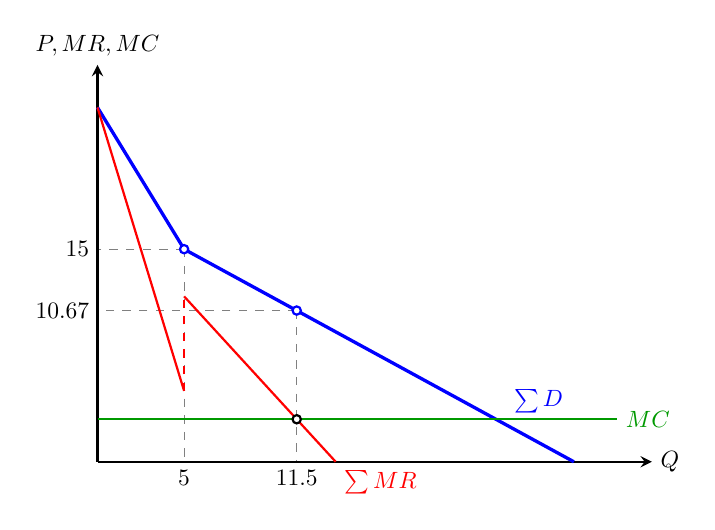
\begin{tikzpicture}[x=0.22cm, y=0.18cm, >=stealth, thick, every node/.style={scale=0.85}]
				% 2. 辅助虚线与防重叠标签
				\draw[dashed, thin, gray] (11.5, 10.67) -- (11.5, 0) node[below, text=black] {$11.5$};
				\draw[dashed, thin, gray] (11.5, 10.67) -- (0, 10.67) node[left, text=black] {$10.67$};
				\draw[dashed, thin, gray] (5, 15) -- (5, 0) node[below, text=black] {$5$};
				\draw[dashed, thin, gray] (5, 15) -- (0, 15) node[left, text=black] {$15$};
				
				% 3. 坐标轴
				\draw[->] (0,0) -- (32,0) node[right] {$Q$};
				\draw[->] (0,0) -- (0,28) node[above] {$P, MR, MC$};
				
				% 4. 绘图代码
				% 水平加总后的总需求折线
				\draw[color=blue, very thick] (0, 25) -- (5, 15) -- (27.5, 0) node[above, yshift=17pt,xshift=-15pt] {$\sum D$};
				
				% 不连续的总边际收益 MR
				\draw[color=red] (0, 25) -- (5, 5);
				\draw[color=red, dashed] (5, 5) -- (5, 11.67); % 断裂跳跃部分
				\draw[color=red] (5, 11.67) -- (13.75, 0) node[below right] {$\sum MR$};
				
				% 边际成本 MC
				\draw[color=green!60!black] (0, 3) -- (30, 3) node[right] {$MC$};
				
				% 5. 均衡点与标号 (fill=white清除交叉线)
				\fill[white] (11.5, 10.67) circle (1.5pt); \draw[blue] (11.5, 10.67) circle (1.5pt); % 定价点
				\fill[white] (11.5, 3) circle (1.5pt); \draw[black] (11.5, 3) circle (1.5pt); % MR=MC 交点
				\fill[white] (5, 15) circle (1.5pt); \draw[blue] (5, 15) circle (1.5pt); % 需求折点
			\end{tikzpicture}
		\end{center}
		\newpage
		\item \textbf{伊丽莎白航空公司（EA）只飞一条航线：芝加哥—檀香山。对这条航线上各航班的需求是 $Q = 500 - P$。伊丽莎白运行各个航班的成本是 $30000$ 美元，增加一位乘客成本增加 $100$ 美元。\\（1）EA的利润最大化价格是什么？每个航班会有多少乘客？EA每个航班的利润是多少？\\（2）伊丽莎白了解到每个航班的固定成本是 $41000$ 美元而不是 $30000$ 美元，它会长期经营下去吗？画一张EA面临的需求曲线，当固定成本为 $30000$ 美元时EA的平均成本曲线，以及当固定成本为 $41000$ 美元时EA的平均成本曲线构成的图来演示你的答案。\\（3）等一下，EA发现有两种不同类型的人飞到檀香山。类型A是需求为 $Q_A = 260 - 0.4P$ 的商务人员。类型B是总需求为 $Q_B = 240 - 0.6P$ 的学生。学生是很容易识别的，所以EA决定对他们定不同的价格。画出各条需求曲线及他们的水平叠加之和。EA给学生定什么价？它对其他乘客定什么价？各航班上各类型乘客各有多少？\\（4）每个航班 EA 的利润将是多少？她还会继续经营下去吗？计算各消费者群体的消费者剩余。总的消费者剩余是多少？\\（5）在 EA 开始实行价格歧视之前，需要到檀香山旅行的类型 A 乘客的消费者剩余是多少？类型 B 呢？为什么总剩余会随着价格歧视而下降，虽然销售总量没有变化？}
		
		\textbf{答：}
		在实行单一垄断定价时，厂商依据边际收益等于边际成本（$MR = MC$）的原则确定最优产销量。根据市场反需求函数 $P = 500 - Q$，可得边际收益 $MR = 500 - 2Q$。令其等于边际成本 $100$ 美元，解得利润最大化乘客数为 $200$ 人，对应均衡价格为 $300$ 美元。此时，航班的总利润为：
		\[
		\begin{aligned}
			\pi = (300 - 100) \times 200 - 30000 = 10000 \text{ 美元}
		\end{aligned}
		\]
		
		当固定成本剧增至 $41000$ 美元时，最优定价与产量并不受影响，但总利润将急剧恶化为 $-1000$ 美元。如图所示，在 $Q = 200$ 处，当固定成本为 $30000$ 美元时，平均成本（$AC_1 = 250$）低于价格，厂商获得标注为蓝色的正向利润矩形；而当固定成本变为 $41000$ 美元时，平均成本（$AC_2 = 305$）反超价格，厂商陷入标注为红色的亏损状态。由于在长期中所有的成本均可变，面对必然的绝对经济亏损，厂商将选择退出市场，停止该航线的运营。
		
		\begin{center}
			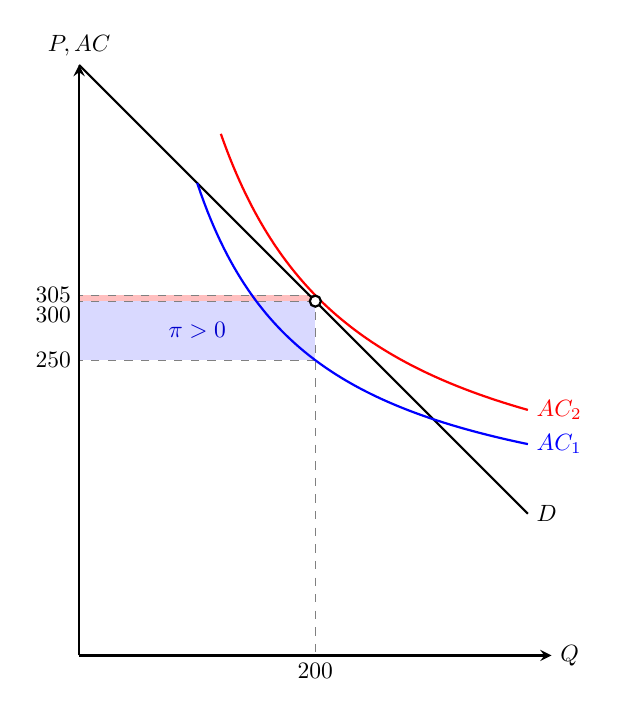
\begin{tikzpicture}[x=0.015cm, y=0.015cm, >=stealth, thick, every node/.style={scale=0.85}]
				% 1. 福利或剩余区域填充
				\fill[blue!15] (0, 250) rectangle (200, 300);
				\fill[red!25] (0, 300) rectangle (200, 305);
				\node[blue!80!black] at (100, 275) {$\pi > 0$};
				
				% 2. 辅助虚线
				\draw[dashed, thin, gray] (200, 305) -- (200, 0) node[below, text=black] {$200$};
				\draw[dashed, thin, gray] (200, 250) -- (0, 250) node[left, text=black] {$250$};
				\draw[dashed, thin, gray] (200, 300) -- (0, 300) node[left, text=black,yshift=-6pt] {$300$};
				\draw[dashed, thin, gray] (200, 305) -- (0, 305) node[left, text=black] {$305$};
				
				% 3. 坐标轴
				\draw[->] (0,0) -- (400,0) node[right] {$Q$};
				\draw[->] (0,0) -- (0,500) node[above] {$P, AC$};
				
				% 4. 绘图代码 (通过同比例缩放除数彻底解决 PGFmath 16384 上限溢出问题)
				\draw[domain=0:380, color=black] plot (\x, {500 - \x}) node[right] {$D$};
				\draw[domain=100:380, color=blue, samples=100] plot (\x, {300/(\x/100) + 100}) node[right] {$AC_1$};
				\draw[domain=120:380, color=red, samples=100] plot (\x, {410/(\x/100) + 100}) node[right] {$AC_2$};
				
				% 5. 交点
				\fill[white] (200, 300) circle (2pt); \draw[black] (200, 300) circle (2pt);
			\end{tikzpicture}
		\end{center}
		
		当厂商能够精准识别不同群体的身份时，便具备了实施三级价格歧视的市场条件。通过反转各自的需求曲线，可得商务人员的反需求函数为 $P_A = 650 - 2.5Q_A$，学生的反需求函数为 $P_B = 400 - \frac{5}{3}Q_B$。令各市场的边际收益等于统一的边际成本 $100$ 美元：
		\[
		\begin{aligned}
			MR_A = 650 - 5Q_A = 100 \quad &\Rightarrow \quad Q_A = 110, \quad P_A = 375 \\
			MR_B = 400 - \frac{10}{3}Q_B = 100 \quad &\Rightarrow \quad Q_B = 90, \quad P_B = 250
		\end{aligned}
		\]
		如图所示，厂商面临的总需求是由两个异质性市场水平加总而成的折线。在实施价格歧视后，厂商向商务人员索要 $375$ 美元的高价，向学生提供 $250$ 美元的折扣价。此时航班的总利润大幅反弹，由于利润重新转正，厂商在固定成本极高的情况下依然能够维持长期经营：
		\[
		\begin{aligned}
			\pi = 375 \times 110 + 250 \times 90 - (41000 + 100 \times 200) = 2750 \text{ 美元}
		\end{aligned}
		\]
		
		\begin{center}
			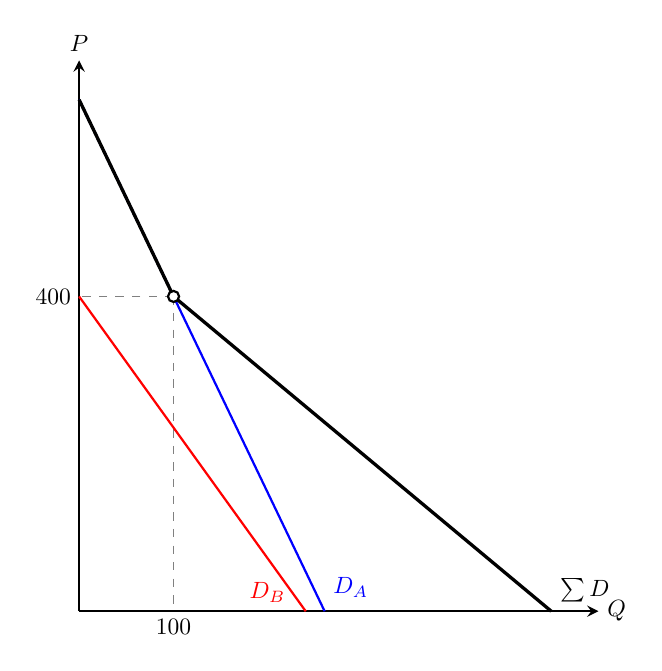
\begin{tikzpicture}[x=0.012cm, y=0.01cm, >=stealth, thick, every node/.style={scale=0.85}]
				% 2. 辅助虚线
				\draw[dashed, thin, gray] (100, 400) -- (100, 0) node[below, text=black] {$100$};
				\draw[dashed, thin, gray] (100, 400) -- (0, 400) node[left, text=black] {$400$};
				
				% 3. 坐标轴
				\draw[->] (0,0) -- (550,0) node[right] {$Q$};
				\draw[->] (0,0) -- (0,700) node[above] {$P$};
				
				% 4. 绘图代码
				\draw[domain=0:260, color=blue] plot (\x, {650 - 2.5*\x}) node[right,yshift=10pt] {$D_A$};
				\draw[domain=0:240, color=red] plot (\x, {400 - 1.667*\x}) node[above left,xshift=-5pt] {$D_B$};
				
				% 水平加总曲线
				\draw[color=black, very thick] (0, 650) -- (100, 400) -- (500, 0) node[above right] {$\sum D$};
				
				% 5. 交点
				\fill[white] (100, 400) circle (2pt); \draw[black] (100, 400) circle (2pt);
			\end{tikzpicture}
		\end{center}
		
		在实行价格歧视时，各群体的消费者剩余分别为：
		\[
		\begin{aligned}
			CS_A &= \frac{1}{2} \times (650 - 375) \times 110 = 15125 \text{ 美元} \\
			CS_B &= \frac{1}{2} \times (400 - 250) \times 90 = 6750 \text{ 美元}
		\end{aligned}
		\]
		全局总剩余为 $21875$ 美元。而在单一统一定价时期（$P=300$），商务人员的消费量为 $140$，学生的消费量仅为 $60$，各群体的消费者剩余为：
		\[
		\begin{aligned}
			CS_A &= \frac{1}{2} \times (650 - 300) \times 140 = 24500 \text{ 美元} \\
			CS_B &= \frac{1}{2} \times (400 - 300) \times 60 = 3000 \text{ 美元}
		\end{aligned}
		\]
		全局总剩余高达 $27500$ 美元。
		
		尽管在这两种定价策略下，航班的售出座位总数严格保持在 $200$ 个，但社会总消费者剩余却随着价格歧视的实施出现了实质性的净损耗。这种现象的经济学本质在于稀缺资源的错配。价格歧视将 $30$ 个座位从边际估值极高的商务人员手中剥夺，并转移给了边际估值较低的学生,损害了消费者的福利。
		\newpage
		
		\item \textbf{影碟租赁采用会员两部收费与无会员单一定价两种模式，分析两部收费原理与双方案设置原因。}
		
		\textbf{答：}
		两部收费制由固定会员费与边际使用费构成。厂商通常将边际费率设定在边际成本（$MC$）以消除无谓损失，再通过收取等于消费者剩余的固定会员费，将其完全转化为垄断利润。然而，在消费者偏好异质且信息不对称的市场中，单一的两部收费制面临两难：高会员费会流失低需求群体，低会员费则无法充分提取高需求群体的剩余。
		
		为此，厂商引入了基于自我选择的菜单甄别机制（二级价格歧视）。如图所示，厂商同时提供两套方案：其一是无会员费的高单价直接租赁模式（$P_S$），该方案满足低需求者的个体理性约束，保留了这部分客群并赚取单次高额溢价；其二是收取较高会员费 $T$ 且单价极低（$P_M = MC$）的会员模式。高需求群体出于总支付成本最小化的动机，满足激励相容约束，将主动选择会员模式。这种双轨制通过不同定价结构的组合，成功诱导消费者按自身类型分流，实现了严格优于单一模式的利润最大化。
		
		\begin{center}
			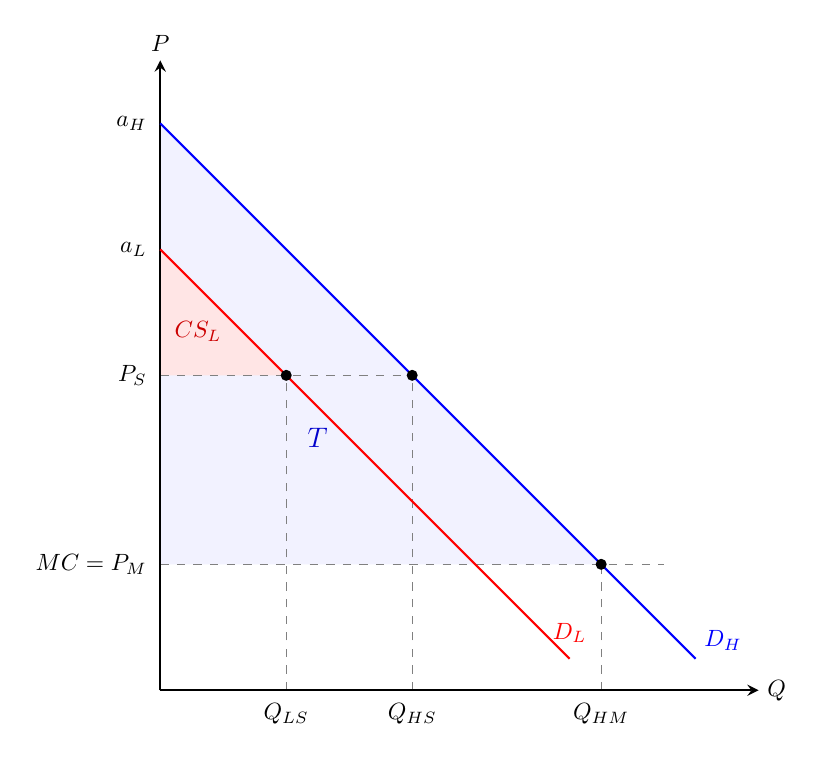
\begin{tikzpicture}[x=0.8cm, y=0.8cm, >=stealth, thick, every node/.style={scale=0.85}]
				% 1. 最底层：福利区域透明填充
				% 会员模式下高需求者的最大剩余（蓝色大三角形）
				\fill[blue!5] (0,2) -- (0,9) -- (7,2) -- cycle; 
				% 单一定价下低需求者获得的剩余（红色小三角形）
				\fill[red!10] (0,5) -- (0,7) -- (2,5) -- cycle; 
				
				% 2. 辅助虚线层 (严格裁切领域)
				\draw[dashed, gray, thin] (0,5) -- (4,5);
				\draw[dashed, gray, thin] (2,0) -- (2,5);
				\draw[dashed, gray, thin] (4,0) -- (4,5);
				\draw[dashed, gray, thin] (0,2) -- (8,2);
				\draw[dashed, gray, thin] (7,0) -- (7,2);
				
				% 3. 坐标轴与防重叠物理标签
				\draw[->] (0,0) -- (9.5,0) node[right] {$Q$};
				\draw[->] (0,0) -- (0,10) node[above] {$P$};
				
				\node[left, xshift=-2pt] at (0,2) {$MC=P_M$};
				\node[left, xshift=-2pt] at (0,5) {$P_S$};
				\node[left, xshift=-2pt] at (0,7) {$a_L$};
				\node[left, xshift=-2pt] at (0,9) {$a_H$};
				
				\node[below, yshift=-2pt] at (2,0) {$Q_{LS}$};
				\node[below, yshift=-2pt] at (4,0) {$Q_{HS}$};
				\node[below, yshift=-2pt] at (7,0) {$Q_{HM}$};
				
				% 4. 供需实线
				\draw[blue] (0,9) -- (8.5,0.5) node[above right, blue] {$D_H$};
				\draw[red] (0,7) -- (6.5,0.5) node[above,yshift=3pt, red] {$D_L$};
				
				% 5. 均衡交点与核心区域代号 (强制清除交叉线干扰)
				\fill[black] (2,5) circle (2pt);
				\fill[black] (4,5) circle (2pt);
				\fill[black] (7,2) circle (2pt);
				
				% 通过坐标微调确保文字不被任何线条遮挡
				\node[text=blue!80!black, font=\large] at (2.5, 4) {$T$};
				\node[text=red!80!black] at (0.6, 5.7) {$CS_L$};
			\end{tikzpicture}
		\end{center}
		
		
		\item \textbf{已知纽约市场需求为 $Q_{NY}=60-0.25P_{NY}$，洛杉矶市场需求为 $Q_{LA}=100-0.5P_{LA}$，总成本为 $C=1000+40Q$。求解实施分市场三级价格歧视与统一定价时的均衡价格、产量及利润，并分析厂商与各市场消费者的福利偏好。}
		
		\textbf{答：}
		三级价格歧视的核心在于基于不同市场的需求价格弹性实施差异化定价。在分隔市场下，厂商遵循边际收益等于边际成本（$MR = MC$）的原则实现利润最大化。根据已知需求，纽约市场的反需求曲线与边际收益曲线分别为
		$$P_{NY} = 240 - 4Q_{NY}\ \ \ \ \ \ MR_{NY} = 240 - 8Q_{NY}$$
		洛杉矶市场分别为
		$$P_{LA} = 200 - 2Q_{LA}\ \ \ \ \ \ MR_{LA} = 200 - 4Q_{LA}$$
		由于 $MC = 40$，分别求解一阶条件：
		\[
		\begin{aligned}
			240 - 8Q_{NY} &= 40 \implies Q_{NY} = 25, \; P_{NY} = 140 \\
			200 - 4Q_{LA} &= 40 \implies Q_{LA} = 40, \; P_{LA} = 120
		\end{aligned}
		\]
		此策略下的总利润为各市场营业利润加总扣除固定成本：$\pi_{sep} = (140 - 40) \times 25 + (120 - 40) \times 40 - 1000 = 4700$。
		
		若实施统一定价，需对两市场需求进行水平加总。总需求函数为 $Q = 160 - 0.75P$。对应的反需求与边际收益函数分别为 
		
		$$P = \frac{640}{3} - \frac{4}{3}Q \ \ \ \ \ \ MR = \frac{640}{3} - \frac{8}{3}Q$$令 $MR = MC = 40$，解得总产量 $Q = 65$，统一均衡价格 $P_U \approx 126.67$。此时两市场销量分别为 $Q_{NY} \approx 28.33, Q_{LA} \approx 36.67$，总利润降为 $\pi_{uni} = (126.67 - 40) \times 65 - 1000 \approx 4633.33$。
		
		各主体的福利偏好受需求弹性差异的严格支配。如图所示，纽约市场需求弹性较小，在价格歧视下承受 $140$ 的高价；统一定价使其价格大幅回落至基准线 $P_U$，消费者剩余扩张，故偏好统一定价。相反，洛杉矶市场需求弹性较大，歧视定价下享有 $120$ 的低价；统一定价使其被迫跨越基准线承受价格上涨（交叉补贴纽约市场），福利受损，故偏好分开定价。对厂商而言，三级价格歧视消除了统一定价带来的妥协漏损，实现了更精准的剩余提取（$\pi_{sep} > \pi_{uni}$），必然偏好分市场定价。
		
		\begin{center}
			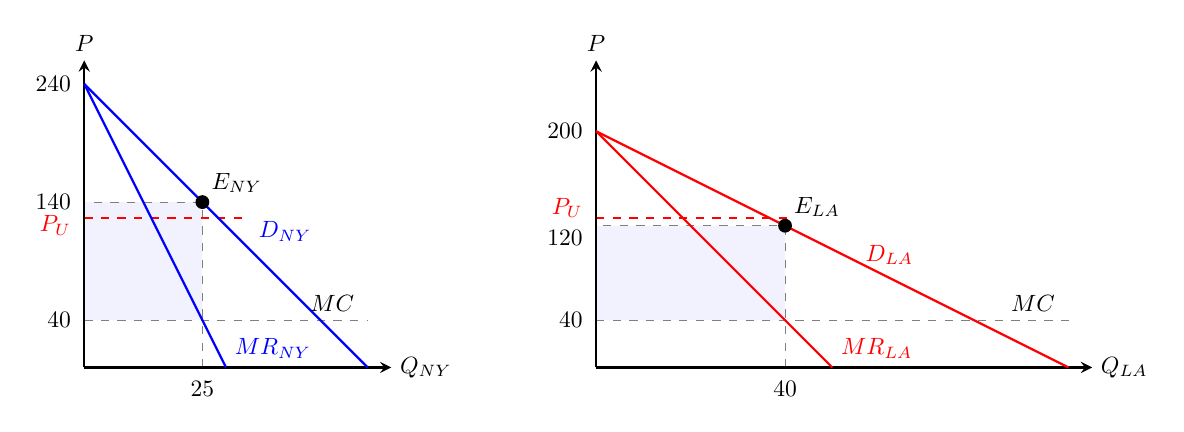
\begin{tikzpicture}[x=0.06cm, y=0.015cm, >=stealth, thick, every node/.style={scale=0.85}]
				% 纽约市场 Scope
				\begin{scope}
					% 1. 透明利润区域填充
					\fill[blue!5] (0,40) rectangle (25,140);
					
					% 2. 辅助虚线与统一定价基准线 (红虚线)
					\draw[dashed, gray, thin] (0, 40) -- (60, 40);
					\draw[dashed, gray, thin] (25, 0) -- (25, 140) -- (0, 140);
					\draw[dashed, red, thick] (0, 126.67) -- (35, 126.67);
					
					% 3. 坐标轴
					\draw[->] (0,0) -- (65,0) node[right] {$Q_{NY}$};
					\draw[->] (0,0) -- (0,260) node[above] {$P$};
					
					% 标签分离 (引入 PU 标签直观显示落差)
					\node[below, yshift=-2pt] at (25,0) {25};
					\node[left, xshift=-2pt] at (0,40) {40};
					\node[left, text=red, xshift=-2pt] at (0,120) {$P_U$};
					\node[left, xshift=-2pt] at (0,140) {140};
					\node[left, xshift=-2pt] at (0,240) {240};
					
					% 4. 供需实线与边际成本线
					\draw[blue] (0,240) -- (60,0) node[above right, blue,yshift=50pt,xshift=-50pt] {$D_{NY}$};
					\draw[blue] (0,240) -- (30,0) node[below right, blue, yshift=16pt] {$MR_{NY}$};
					\node[above, xshift=5pt] at (50,40) {$MC$};
					
					% 5. 均衡点与标号
					\fill[black] (25,140) circle (2.5pt) node[fill=white, inner sep=1.5pt, above right, xshift=2pt, yshift=2pt] {$E_{NY}$};
				\end{scope}
				
				% 洛杉矶市场 Scope
				\begin{scope}[xshift=6.5cm]
					% 1. 透明利润区域填充
					\fill[blue!5] (0,40) rectangle (40,120);
					
					% 2. 辅助虚线与统一定价基准线 (红虚线)
					\draw[dashed, gray, thin] (0, 40) -- (100, 40);
					\draw[dashed, gray, thin] (40, 0) -- (40, 120) -- (0, 120);
					\draw[dashed, red, thick] (0, 126.67) -- (50, 126.67);
					
					% 3. 坐标轴
					\draw[->] (0,0) -- (105,0) node[right] {$Q_{LA}$};
					\draw[->] (0,0) -- (0,260) node[above] {$P$};
					
					% 标签分离
					\node[below, yshift=-2pt] at (40,0) {40};
					\node[left, xshift=-2pt] at (0,40) {40};
					\node[left, xshift=-2pt] at (0,110) {120};
					\node[left, text=red, xshift=-2pt] at (0,135) {$P_U$};
					\node[left, xshift=-2pt] at (0,200) {200};
					
					% 4. 供需实线与边际成本线
					\draw[red] (0,200) -- (100,0) node[above right, red,yshift=40pt,xshift=-90pt] {$D_{LA}$};
					\draw[red] (0,200) -- (50,0) node[below right, red, yshift=16pt] {$MR_{LA}$};
					\node[above, xshift=5pt] at (90,40) {$MC$};
					
					% 5. 均衡点与标号
					\fill[black] (40,120) circle (2.5pt) node[fill=white, inner sep=1.5pt, above right, xshift=2pt, yshift=2pt] {$E_{LA}$};
				\end{scope}
			\end{tikzpicture}
		\end{center}
		
		\item \textbf{你是出租超级计算机的超级计算机公司（SC）的执行官。SC 出租计算机每次可以得到一个固定的租费（与使用时间无关），并从每秒钟的使用时间中收费 P 美分。SC 有相同数目的两类潜在顾客——10 家企业和 10 个学术机构。各家企业客户有需求函数 $Q = 10 - P$，其中 Q 以每月百万秒计；各学术机构有需求函数 $Q = 8 - P$。SC 增加的计算时间的边际成本为每秒 2 美分，不管总量是多少。\\（1）假设你能将企业和学术机构分开，你对各组要的租费和使用费各是多少？你的利润是多少？\\（2）假设你无法把两类客户分开，且你不要租费，使你利润最大的使用费是多少？你的利润又是多少？\\（3）假设你定一种两部收费，即定一种企业客户和学术机构客户共同的租费和使用费。你所定的使用费和租费各为多少？你的利润是多少？解释为什么价格不等于边际成本。}
		
		\textbf{答：}
		如果厂商能够完全甄别企业与学术机构并实施隔离定价，为实现利润最大化，应当向两类群体分别制定最优的两部收费策略。由于不存在跨群体的信息不对称限制，最优策略是将使用费严格设定为等于边际成本（$P=MC=2$ 美分/秒），并利用固定的租费将两类群体在该价格下所获得的消费者剩余全额榨取。对于学术机构，在 $P=2$ 时对应的租费为：
		\[
		\begin{aligned}
			T_A = \frac{1}{2} \times (8 - 2) \times (8 - 2) = 18 \text{ 百万美分/月} = 180000 \text{ 美元/月}
		\end{aligned}
		\]
		对于企业客户，在 $P=2$ 时对应的租费为：
		\[
		\begin{aligned}
			T_B = \frac{1}{2} \times (10 - 2) \times (10 - 2) = 32 \text{ 百万美分/月} = 320000 \text{ 美元/月}
		\end{aligned}
		\]
		此时，每秒的边际使用利润为零，厂商的所有可变利润均来源于租费。总利润为：
		\[
		\begin{aligned}
			\pi = 10 \times 180000 + 10 \times 320000 - FC = 5000000 - FC \text{ （美元/月）}
		\end{aligned}
		\]
		
		如果无法将两类客户分开且被迫放弃两部收费（即仅收取单一的使用费），厂商面临的总需求为两类客户需求的水平加总。总需求函数与反需求函数为：
		\[
		\begin{aligned}
			Q &= 10(10 - P) + 10(8 - P) = 180 - 20P \\
			P &= 9 - \frac{Q}{20}
		\end{aligned}
		\]
		构建厂商的利润函数并根据一阶最优化条件（$MR = MC$）求解：
		\[
		\begin{aligned}
			\pi &= \left(9 - \frac{Q}{20}\right)Q - 2Q \\
			\frac{\mathrm{d}\pi}{\mathrm{d}Q} &= 7 - \frac{Q}{10} = 0 \quad \Rightarrow \quad Q = 70
		\end{aligned}
		\]
		将其代回反需求函数，解得最优使用费为 $P = 5.5$ 美分/秒。此时的最大利润为 $(5.5 - 2) \times 70 = 245$ 百万美分/月（即 $2.45$ 百万美元/月）。
		
		如果采用针对全市场的统一两部收费策略，由于必须兼顾学术机构与企业客户，租费 $T$ 必须受限于需求较弱的学术机构的保留消费者剩余。如果将租费定得过高（如等于企业客户的剩余），学术机构将彻底退出市场。因此，对于任意使用费 $P^*$，租费的理论上限为：
		\[
		\begin{aligned}
			T = CS_A = \frac{1}{2}(8 - P^*)^2
		\end{aligned}
		\]
		厂商的总利润函数由 $20$ 家客户的固定租费以及总产量的边际使用费加成两部分构成：
		\[
		\begin{aligned}
			\pi &= 20T + (P^* - MC)(Q_A + Q_B) \\
			&= 10(8 - P^*)^2 + (P^* - 2)(180 - 20P^*)
		\end{aligned}
		\]
		对 $P^*$ 求导以求极值：
		\[
		\begin{aligned}
			\frac{\mathrm{d}\pi}{\mathrm{d}P^*} = -20P^* + 60 = 0 \quad \Rightarrow \quad P^* = 3 \text{ 美分/秒}
		\end{aligned}
		\]
		将最优使用费代回租费公式，解得租费 $T = 12.5$ 百万美分/月（即 $125000$ 美元/月）。此时整体的最大化利润为 $370$ 百万美分/月（即 $3.70$ 百万美元/月）。
		
		在这种混合两部收费均衡中，价格并没有等于边际成本（$P^* > MC$）。如图所示，其微观经济学原理在于厂商为了平衡从高需求者那里提取剩余的效率。当使用费从 $MC$ 稍微提高时，厂商虽然在每个客户身上损失了与提价幅度等比的固定租费（蓝色三角形面积缩小），但却能从高需求群体（企业客户）更为庞大的消费量中获得额外的边际使用利润的补偿。当边际租费损失等于边际使用费收益时，利润达到全局最大化。
		
		\begin{center}
			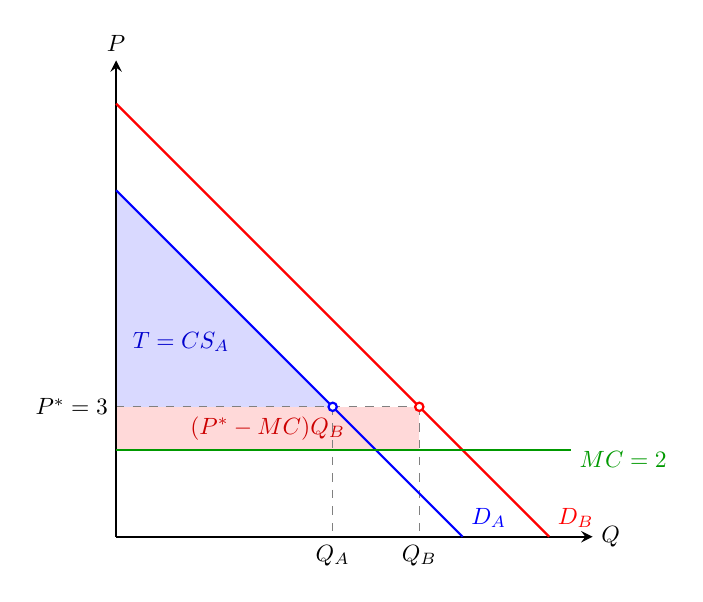
\begin{tikzpicture}[x=0.55cm, y=0.55cm, >=stealth, thick, every node/.style={scale=0.85}]
				% 1. 区域填充 (底层)
				\fill[blue!15] (0, 8) -- (0, 3) -- (5, 3) -- cycle;
				\node[blue!80!black] at (1.5, 4.5) {$T = CS_A$};
				
				\fill[red!15] (0, 3) rectangle (7, 2);
				\fill[red!15] (0, 2) rectangle (5, 3);
				\node[red!80!black] at (3.5, 2.5) {$(P^*-MC)Q_B$};
				
				% 2. 辅助虚线
				\draw[dashed, thin, gray] (5, 3) -- (5, 0) node[below, text=black] {$Q_A$};
				\draw[dashed, thin, gray] (7, 3) -- (7, 0) node[below, text=black] {$Q_B$};
				\draw[dashed, thin, gray] (0, 3) node[left, text=black] {$P^*=3$} -- (7, 3);
				
				% 3. 坐标轴
				\draw[->] (0,0) -- (11,0) node[right] {$Q$};
				\draw[->] (0,0) -- (0,11) node[above] {$P$};
				
				% 4. 绘图代码
				\draw[domain=0:8, color=blue] plot (\x, {8 - \x}) node[above right] {$D_A$};
				\draw[domain=0:10, color=red] plot (\x, {10 - \x}) node[above right] {$D_B$};
				\draw[domain=0:10.5, color=green!60!black] plot (\x, {2}) node[right, yshift=-4pt] {$MC=2$};
				
				% 5. 交点
				\fill[white] (5, 3) circle (1.5pt); \draw[blue] (5, 3) circle (1.5pt);
				\fill[white] (7, 3) circle (1.5pt); \draw[red] (7, 3) circle (1.5pt);
			\end{tikzpicture}
		\end{center}
		
		\item \textbf{作为一孤立的富裕社区惟一的网球俱乐部的拥有者，你必须决定会员费和场地时间费。有两种类型的网球手：“网球发烧友”的需求为 $Q_1 = 10 - P$，其中 $Q_1$ 为每周场地小时；P 为每人每小时的费用。“散客”球手的需求为 $Q_2 = 4 - 0.25P$。设各类型都有 1000 人。你有足够的场地，因而场地时间的边际成本为 0。你有每周 10000 美元的固定成本。“网球发烧友”和“散客”球手看上去是类似，所以你必须给他们定同样的价格。\\（1）假设为了保持一种“职业”气氛，你想将会员限制在“网球发烧友”。你将如何定年度会员费和场地费（假设每年为52周）以使利润最大化？（记住，只有那些热衷的网球手才会选择入会的限制）。\\（2）有个朋友告诉你鼓励两类网球手都入会将能赚的利润更多。这个朋友说的是否有道理？多少年费和场地费，会使周利润最大化？利润是多少？\\（3）假设过了几年，年轻的、进取的专业人员搬到你的社区，他们都是“网球发烧友”。你相信现在有3000个“网球发烧友”和1000个“散客”球手。对“散客”球手开放还有利可图吗？利润最大化的年会费和场地费是多少？每周利润是多少？}
		
		\textbf{答：}
		如果俱乐部的战略是将所有会员严格限制在核心网球发烧友群体中，其相当于面临单一的同质化需求市场。为了实现利润最大化，应当将边际场地费定为边际成本（由于产能充足，$P=MC=0$），并将全部的消费者剩余作为会员费予以榨取。在 $P=0$ 时，发烧友每周的消费者剩余为：
		\[
		\begin{aligned}
			T = \frac{1}{2} \times 10 \times 10 = 50 \text{ 美元/周}
		\end{aligned}
		\]
		将其折算为年度会员费为 $50 \times 52 = 2600$ 美元。此时俱乐部的每周总利润为 $(50 \times 1000) - 10000 = 40000$ 美元。
		
		朋友的建议在经济学上是完全成立的，因为异质性市场的混合两部收费往往能越过单一市场排斥策略的利润边界。如图所示，偶尔参与的散客具有极高的初始保留价格（$P=16$），但需求衰减极快；而发烧友需求相对平缓且规模庞大。为了将两类群体同时纳入会员体系，俱乐部必须将每周会员费 $T$ 设定为需求较弱者（散客）在特定使用费 $P$ 下的剩余：
		\[
		\begin{aligned}
			T = CS_2 = \frac{1}{2} \times Q_2 \times (16 - P) = \frac{1}{2}(4 - 0.25P)(16 - P) = 32 - 4P + \frac{1}{8}P^2
		\end{aligned}
		\]
		此时，面向 $2000$ 名混合会员的总收入 $TR$ 为会员费与场地费之和：
		\[
		\begin{aligned}
			TR &= 2000T + P(1000Q_1 + 1000Q_2) \\
			&= 2000\left(32 - 4P + \frac{1}{8}P^2\right) + 1000P(14 - 1.25P) \\
			&= 1000(64 + 6P - P^2)
		\end{aligned}
		\]
		构建周利润函数并求解一阶最大化条件：
		\[
		\begin{aligned}
			\pi &= 1000(64 + 6P - P^2) - 10000 \\
			\frac{\mathrm{d}\pi}{\mathrm{d}P} &= 1000(6 - 2P) = 0 \quad \Rightarrow \quad P = 3 \text{ 美元/小时}
		\end{aligned}
		\]
		将最优使用费代入，解得年度会员费为 $(32 - 12 + 1.125) \times 52 = 1098.5$ 美元，对应的每周最大化利润大幅跃升至 $63000$ 美元，显著优于仅限制发烧友入会的利润水平。
		
		\begin{center}
			\begin{tikzpicture}[x=0.75cm, y=0.35cm, >=stealth, thick, every node/.style={scale=0.85}]
				% 1. 区域填充
				\fill[orange!15] (0, 16) -- (0, 3) -- (3.25, 3) -- cycle;
				\node[orange!80!black] at (1, 6.5) {$T = CS_2$};
				
				% 2. 辅助虚线
				\draw[dashed, thin, gray] (3.25, 3) -- (3.25, 0) node[below, text=black] {$3.25$};
				\draw[dashed, thin, gray] (7, 3) -- (7, 0) node[below, text=black] {$7$};
				\draw[dashed, thin, gray] (0, 3) node[left, text=black] {$P^*=3$} -- (7, 3);
				
				% 3. 坐标轴
				\draw[->] (0,0) -- (11,0) node[right] {$Q$};
				\draw[->] (0,0) -- (0,18) node[above] {$P$};
				
				% 4. 绘图代码
				\draw[domain=0:10, color=blue] plot (\x, {10 - \x}) node[above,yshift=8pt] {$D_1$ (发烧友)};
				\draw[domain=0:4, color=red] plot (\x, {16 - 4*\x}) node[right,yshift=10pt] {$D_2$ (散客)};
				\draw[domain=0:10.5, color=green!60!black] plot (\x, {0}) node[below, yshift=-4pt] {$MC=0$};
				
				% 5. 交点
				\fill[white] (3.25, 3) circle (1.5pt); \draw[red] (3.25, 3) circle (1.5pt);
				\fill[white] (7, 3) circle (1.5pt); \draw[blue] (7, 3) circle (1.5pt);
			\end{tikzpicture}
		\end{center}
		
		当人口结构发生剧变，高需求的发烧友扩张至 $3000$ 人时，我们需要重新评估战略。若退回仅限制发烧友入会的排他策略（即 $P=0, T=50$），凭借人口红利，周利润能够达到 $(50 \times 3000) - 10000 = 140000$ 美元。
		若继续向散客开放并实施混合两部收费，总收益函数将重构为：
		\[
		\begin{aligned}
			TR &= 4000T + P(3000Q_1 + 1000Q_2) \\
			&= 4000\left(32 - 4P + \frac{1}{8}P^2\right) + 1000P\left[3(10 - P) + (4 - 0.25P)\right] \\
			&= 1000(128 + 18P - 2.75P^2)
		\end{aligned}
		\]
		求解新的利润最大化条件：
		\[
		\begin{aligned}
			\frac{\mathrm{d}\pi}{\mathrm{d}P} = 1000(18 - 5.5P) = 0 \quad \Rightarrow \quad P \approx 3.27 \text{ 美元/小时}
		\end{aligned}
		\]
		将最优使用费代入，解得包含所有群体的最大化周利润为 $147455$ 美元。由于 $147455 > 140000$，即使发烧友在绝对基数上占据了压倒性优势，只要通过精算上调边际使用费（从 $3$ 美元升至 $3.27$ 美元）来动态挤压散客剩余并提取发烧友的增量价值，对散客保持开放依然是实现全局最优的有利可图之举。
		\newpage
		
		\item \textbf{图 11.15 反映了三个消费者对两种产品的保留价格。假设两种产品的边际生产成本都是零，生产商能通过分开出售、捆绑销售或混合捆绑销售（即既分开供应也捆绑销售）能赚到最多的钱吗？价格应怎么定？}
		
		\textbf{答：}
		基于消费者对两种产品的保留价格（表 1），可分别计算三种定价策略的利润最大化均衡。
		
		\begin{center}
			\renewcommand{\arraystretch}{1.1}
			\begin{tabular}{lccc}
				\toprule
				消费者 & 产品 1 ($r_1$) & 产品 2 ($r_2$) & 捆绑总估值 ($r_1+r_2$) \\
				\midrule
				消费者 A & 3.25 & 6.00 & 9.25 \\
				消费者 B & 8.25 & 3.25 & 11.50 \\
				消费者 C & 10.00 & 10.00 & 20.00 \\
				\bottomrule
			\end{tabular}
		\end{center}
		
		在分开销售策略下，厂商需对产品 1 和 2 分别独立定价。由数据可知，最优单独定价为 $P_1 = 8.25$ 与 $P_2 = 6.00$。此时消费者 B、C 购买产品 1，消费者 A、C 购买产品 2。总销售量各为 2 单位，实现利润 $2 \times 8.25 + 2 \times 6.00 = 28.50$。
		
		在纯捆绑销售策略下，消费者只能以统一价格购买消费束。由于厂商追求利润最大化，且边际成本为零，最优捆绑价格由最低总估值决定，即 $P_B = 9.25$。所有消费者均购买该消费束，实现总利润 $3 \times 9.25 = 27.75$。
		
		在混合捆绑销售策略下，厂商同时提供单品与消费束。最优定价组合为 $P_1 = 10.00, P_2 = 6.00, P_B = 11.50$。此时，消费者 A 选择单独购买产品 2（获得剩余为 $0$），消费者 B 与 C 均选择购买捆绑消费束。均衡利润为：
		\[
		\begin{aligned}
			\pi_{mixed} = P_2 + 2P_B = 6.00 + 2 \times 11.50 = 29.00
		\end{aligned}
		\]
		
		比较三种策略，混合捆绑销售产生的利润最高。当不同消费者的需求呈现非完全的负相关性，且边际成本较低时，混合捆绑销售能通过诱导极端偏好者购买单品、中间偏好者购买消费束，实现更优的价格歧视与剩余提取。
		
		\begin{center}
			\begin{tikzpicture}[x=0.55cm, y=0.55cm, >=stealth, thick, every node/.style={scale=0.85}]
				% 辅助虚线
				\draw[dashed, gray, thin] (3.25, 0) -- (3.25, 6) -- (0, 6);
				\draw[dashed, gray, thin] (8.25, 0) -- (8.25, 3.25) -- (0, 3.25);
				\draw[dashed, gray, thin] (10, 0) -- (10, 10) -- (0, 10);
				
				% 坐标轴
				\draw[->] (0,0) -- (12,0) node[right] {$r_1$};
				\draw[->] (0,0) -- (0,12) node[above] {$r_2$};
				
				% 标签与坐标点物理分离
				\node[below, yshift=-2pt] at (3.25, 0) {3.25};
				\node[below, yshift=-2pt] at (8.25, 0) {8.25};
				\node[below, yshift=-2pt] at (10, 0) {10.00};
				
				\node[left, xshift=-2pt] at (0, 3.25) {3.25};
				\node[left, xshift=-2pt] at (0, 6) {6.00};
				\node[left, xshift=-2pt] at (0, 10) {10.00};
				
				% 绘制散点
				\fill[black] (3.25, 6) circle (2.5pt) node[fill=white, inner sep=1.5pt, above left, xshift=-2pt, yshift=2pt] {A};
				\fill[black] (8.25, 3.25) circle (2.5pt) node[fill=white, inner sep=1.5pt, above right, xshift=2pt, yshift=2pt] {B};
				\fill[black] (10, 10) circle (2.5pt) node[fill=white, inner sep=1.5pt, above right, xshift=2pt, yshift=2pt] {C};
			\end{tikzpicture}
		\end{center}
		
		\newpage
		\item \textbf{回到图 11.16。设边际成本 $c_1$ 和 $c_2$ 为零，证明在这种情况下纯捆绑销售是最有利可图的定价策略，而不是混合捆绑销售。这个捆绑销售应该定价多少？而厂商的利润是多少？}
		
		\textbf{答：}
		如图所示，四位消费者的保留价格呈现完全的负相关性，其对两种产品的总估值均严格等于 $100$（见表 2）。
		
		\begin{center}
			\renewcommand{\arraystretch}{1.1}
			\begin{tabular}{lccc}
				\toprule
				消费者 & 产品 1 ($r_1$) & 产品 2 ($r_2$) & 捆绑总估值 ($r_1+r_2$) \\
				\midrule
				消费者 A & 10 & 90 & 100 \\
				消费者 B & 50 & 50 & 100 \\
				消费者 C & 60 & 40 & 100 \\
				消费者 D & 90 & 10 & 100 \\
				\bottomrule
			\end{tabular}
		\end{center}
		
		在边际成本为零的前提下，厂商实现利润最大化的充分必要条件是最大程度地提取消费者总剩余。由于所有消费者对组合的总保留价格均相同（均为 $100$），厂商只需设定统一的纯捆绑销售价格 $P_B = 100$。此时，所有四位消费者均会购买消费束，厂商成功将所有消费者剩余转化为利润，总利润达到最大化：
		\[
		\begin{aligned}
			\pi_{pure} = 4 \times P_B = 400
		\end{aligned}
		\]
		
		若采用混合捆绑或单独销售，为诱使消费者分别购买单品，单品定价必须低于其对应保留价格，这必然导致部分消费者剩余无法被厂商完全提取（例如单独销售设定 $P_1=50, P_2=50$ 时，总利润仅为 $250$）。因此，当需求完全负相关且边际成本为零时，纯捆绑销售能实现完全价格歧视，是严格优于混合捆绑的最优策略。
		
		\begin{center}
			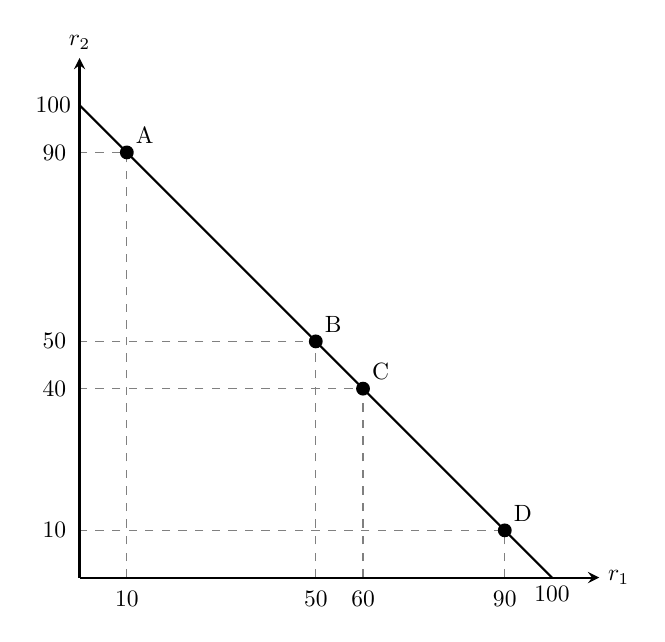
\begin{tikzpicture}[x=0.06cm, y=0.06cm, >=stealth, thick, every node/.style={scale=0.85}]
				% 辅助虚线
				\draw[dashed, gray, thin] (10, 0) -- (10, 90) -- (0, 90);
				\draw[dashed, gray, thin] (50, 0) -- (50, 50) -- (0, 50);
				\draw[dashed, gray, thin] (60, 0) -- (60, 40) -- (0, 40);
				\draw[dashed, gray, thin] (90, 0) -- (90, 10) -- (0, 10);
				
				% 坐标轴
				\draw[->] (0,0) -- (110,0) node[right] {$r_1$};
				\draw[->] (0,0) -- (0,110) node[above] {$r_2$};
				
				\node[below, yshift=-2pt] at (10, 0) {10};
				\node[below, yshift=-2pt] at (50, 0) {50};
				\node[below, yshift=-2pt] at (60, 0) {60};
				\node[below, yshift=-2pt] at (90, 0) {90};
				
				\node[left, xshift=-2pt] at (0, 10) {10};
				\node[left, xshift=-2pt] at (0, 40) {40};
				\node[left, xshift=-2pt] at (0, 50) {50};
				\node[left, xshift=-2pt] at (0, 90) {90};
				
				% 需求等值线 r1+r2=100
				\draw[black, thick] (0, 100) node[left] {100} -- (100, 0) node[below] {100};
				
				% 绘制散点
				\fill[black] (10, 90) circle (2.5pt) node[fill=white, inner sep=1.5pt, above right, xshift=2pt, yshift=2pt] {A};
				\fill[black] (50, 50) circle (2.5pt) node[fill=white, inner sep=1.5pt, above right, xshift=2pt, yshift=2pt] {B};
				\fill[black] (60, 40) circle (2.5pt) node[fill=white, inner sep=1.5pt, above right, xshift=2pt, yshift=2pt] {C};
				\fill[black] (90, 10) circle (2.5pt) node[fill=white, inner sep=1.5pt, above right, xshift=2pt, yshift=2pt] {D};
			\end{tikzpicture}
		\end{center}
		
		\newpage
		\item \textbf{许多年前，《纽约时报》上出现一篇关于 IBM 的定价政策的文章。此前一天 IBM 宣布对他的大多数中小型计算机削价。文章说：IBM 要使得它的顾客更多购买而较少租赁计算机，除了定期降价外大概别无选择。如果它们成功了，这就会使得 IBM 的主要竞争者的日子更难过。摩根斯坦利的奥列克·韦尔（Ulric Weil）在他的新书《80 年代的信息系统》中这样说道：“计算机的买断是不断扩大的 IBM 的收益和利润所必需的。”韦尔宣称，IBM 不可能再恢复到强调租赁的时代。\\
			（1）提供一个简短但清楚的支持 IBM 应该试图 “使顾客更多购买而较少租赁” 的声明的论证。\\
			（2）提出一个简短但清楚的反对该声明的论证。\\
			（3）什么因素决定，究竟是租赁还是销售，对像 IBM 这样的公司更有利？试做简短解释。}
		
		\textbf{答：}
		（1）支持销售（买断）策略的核心经济学逻辑在于锁定效应、战略防御与风险转移。直接购买需要投入高昂的初始沉没成本，这在无形中构建了极高的转换壁垒，将客户牢牢锁定在 IBM 的技术生态内，有效阻断了竞争对手后续的市场渗透。同时，计算机硬件具有极高的技术迭代风险与折旧速度，通过出售设备，IBM 得以将资产快速贬值的风险完全转嫁给消费者。
		
		（2）反对销售（支持租赁）的核心逻辑在于两部收费制的实施潜力。作为拥有市场势力的垄断厂商，IBM 若采用租赁模式，可通过对设备使用量进行计量（收取固定基础租金与按时间/计算量计价的边际使用费），实施二级价格歧视。这种基于高频使用者榨取额外消费者剩余的机制，在一次性直接买断模式中是无法实现的。
		
		（3）企业在租赁与销售间的帕累托最优决策主要取决于以下三大核心要素的权衡：
		\begin{enumerate}
			\item \textbf{价格歧视的剩余榨取空间}：通过租赁衍生的两部收费制所捕获的消费者剩余总量，是否显著超过一次性销售带来的即期利润。
			\item \textbf{相对贴现率差异}：若 IBM 的内部资金贴现率高于其目标客户群的贴现率，即期回笼大量现金流的销售模式更具吸引力；反之则倾向于长期获取租赁稳定现金流。
			\item \textbf{市场结构的脆弱性与进入威胁}：当面临竞争对手强烈的进入威胁时，直接出售能迅速抢占并固化市场份额，构建用户转换壁垒；若自身处于稳固的绝对垄断地位，则更倾向于通过租赁追求长期剩余最大化。
		\end{enumerate}
		
		\item \textbf{你在一个有三个消费者组成的市场上销售产品 1 和产品 2。三个消费者的保留价格如下表所示。各产品的单位成本为 30 美元。（1）对分开销售两种产品、纯捆绑销售和混合捆绑销售，分别计算价格和利润。（2）哪种策略是最有利可图的？为什么？}
		
		\textbf{答：}
		基于给定条件，三个消费者对产品的保留价格与捆绑总估值分布如下：
		
		\begin{center}
			\renewcommand{\arraystretch}{1.1}
			\begin{tabular}{lccc}
				\toprule
				消费者 & 产品 1 ($r_1$) & 产品 2 ($r_2$) & 捆绑总估值 ($r_1+r_2$) \\
				\midrule
				消费者 A & 20 & 100 & 120 \\
				消费者 B & 60 & 60 & 120 \\
				消费者 C & 100 & 20 & 120 \\
				\bottomrule
			\end{tabular}
		\end{center}
		
		在分开销售策略下，由于边际成本 $MC=30$，为实现利润最大化，厂商对产品 1 和 2 的最优独立定价均为 $P_1 = P_2 = 100$。此时，仅消费者 C 购买产品 1，仅消费者 A 购买产品 2。均衡总利润为：
		\[
		\begin{aligned}
			\pi_{sep} = (100 - 30) \times 1 + (100 - 30) \times 1 = 140
		\end{aligned}
		\]
		
		在纯捆绑销售策略下，厂商以统一价格销售包含两件产品的消费束。此时捆绑边际成本为 $30+30=60$。由于所有消费者的总估值均为 120，最优捆绑价格 $P_B = 120$。
		
		全体消费者均购买消费束，均衡总利润为：
		\[
		\begin{aligned}
			\pi_{pure} = 3 \times (120 - 60) = 180
		\end{aligned}
		\]
		
		在混合捆绑销售策略下，厂商需通过精巧的价格组合实现自我选择（Self-selection）。为最大化提取剩余，厂商设定 $P_B = 120$ 以锁定中间偏好者 B，同时为诱导极端偏好者 A 和 C 仅购买单品，单品定价必须满足激励相容约束：消费者购买单品的剩余必须严格大于购买消费束的剩余。以消费者 A 为例，需满足 $r_2 - P_2 > (r_1+r_2) - P_B$，即 $100 - P_2 > 120 - 120 = 0$。因此，设定极限逼近价格 $P_1 = P_2 = 99.95$。在此组合下，A 仅购买产品 2，C 仅购买产品 1，B 购买消费束。均衡总利润为：
		\[
		\begin{aligned}
			\pi_{mixed} = 2 \times (99.95 - 30) + (120 - 60) = 199.90
		\end{aligned}
		\]
		
		混合捆绑销售是最有利可图的策略。其核心经济学机制在于规避了无谓损失。由于产品的边际成本（30 美元）高于消费者 A 对产品 1 的保留价格（20 美元）以及 C 对产品 2 的保留价格（20 美元），纯捆绑销售强制向其搭售低估值产品，产生了“生产成本高于支付意愿”的效率漏损。混合捆绑销售通过设定诱导性的单品价格，成功将这部分低效配置剥离，实现了最优的价格歧视。
		
		\begin{center}
			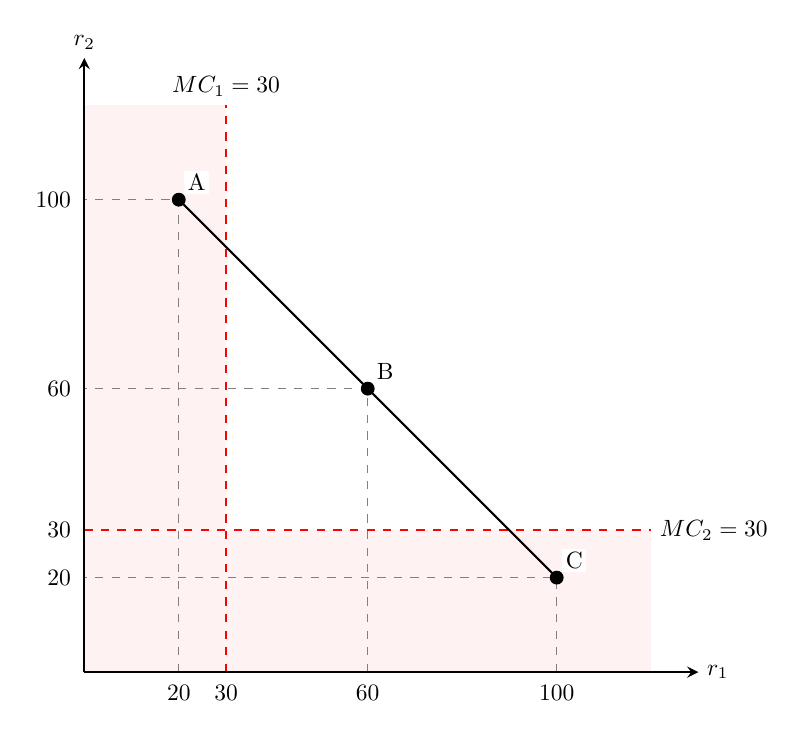
\begin{tikzpicture}[x=0.06cm, y=0.06cm, >=stealth, thick, every node/.style={scale=0.85}]
				% 底层透明填充 (低效交易区域)
				\fill[red!5] (0,0) rectangle (30, 120);
				\fill[red!5] (0,0) rectangle (120, 30);
				
				% 辅助虚线
				\draw[dashed, gray, thin] (20, 0) -- (20, 100) -- (0, 100);
				\draw[dashed, gray, thin] (60, 0) -- (60, 60) -- (0, 60);
				\draw[dashed, gray, thin] (100, 0) -- (100, 20) -- (0, 20);
				
				% 边际成本线
				\draw[dashed, red, thick] (30, 0) -- (30, 120) node[above, black] {$MC_1=30$};
				\draw[dashed, red, thick] (0, 30) -- (120, 30) node[right, black] {$MC_2=30$};
				
				% 坐标轴
				\draw[->] (0,0) -- (130,0) node[right] {$r_1$};
				\draw[->] (0,0) -- (0,130) node[above] {$r_2$};
				
				\node[below, yshift=-2pt] at (20, 0) {20};
				\node[below, yshift=-2pt] at (30, 0) {30};
				\node[below, yshift=-2pt] at (60, 0) {60};
				\node[below, yshift=-2pt] at (100, 0) {100};
				
				\node[left, xshift=-2pt] at (0, 20) {20};
				\node[left, xshift=-2pt] at (0, 30) {30};
				\node[left, xshift=-2pt] at (0, 60) {60};
				\node[left, xshift=-2pt] at (0, 100) {100};
				
				% 需求等值线
				\draw[black, thick] (20, 100) -- (100, 20);
				
				% 绘制散点
				\fill[black] (20, 100) circle (2.5pt) node[fill=white, inner sep=1.5pt, above right, xshift=2pt, yshift=2pt] {A};
				\fill[black] (60, 60) circle (2.5pt) node[fill=white, inner sep=1.5pt, above right, xshift=2pt, yshift=2pt] {B};
				\fill[black] (100, 20) circle (2.5pt) node[fill=white, inner sep=1.5pt, above right, xshift=2pt, yshift=2pt] {C};
			\end{tikzpicture}
		\end{center}
		
		
		\item \textbf{你的企业生产两种产品，对它们的需求是相互独立的。两种产品生产的边际成本都是零。你面临有下列保留价格的四个消费者：A (25, 100), B (40, 80), C (80, 40), D (100, 25)。\\
			（1）考虑分开销售、纯捆绑销售和混合捆绑销售三种策略，确定最优定价和相应的利润。哪种策略最好？\\
			（2）现在假设每种产品的生产都有 30 美元的边际成本。答案会怎样变化？为什么最优策略不同了？}
		
		\textbf{答：}
		基于消费者特征，其对两种产品的保留价格与捆绑总估值 ($r_1+r_2$) 分布如下：A 估值为 125，B 估值为 120，C 估值为 120，D 估值为 125。
		
		在边际成本为零的基准情形下，分开销售的最优策略为 $P_1 = 80, P_2 = 80$，此时各售出两单位（销售量分别由 C、D 和 A、B 贡献），总利润为 $2 \times 80 + 2 \times 80 = 320$。纯捆绑销售的最优定价受制于最低总估值，即 $P_B = 120$，四位消费者全部购买，实现利润 $4 \times 120 = 480$。混合捆绑销售由于必须设定略微低于保留价格的单品价格（如 $P_1 = P_2 = 94.95, P_B = 120$）以过滤需求，均衡利润为 $429.90$。因此，当边际成本为零时，纯捆绑销售是最优策略。其核心逻辑在于，零边际成本意味着没有任何供给构成了效率损失，厂商只需单纯追求剥夺全市场最大公约数的总剩余即可。
		
		引入 30 美元的边际成本后，机制发生显著改变。分开销售在 $P_1 = P_2 = 80$ 时，总利润降为 $2 \times (80-30) + 2 \times (80-30) = 200$。纯捆绑销售在 $P_B = 120$ 时，捆绑成本升至 60，利润降为 $4 \times (120-60) = 240$。
		
		混合捆绑销售在此阶段凸显出绝对优势。厂商设定 $P_B = 120$。此时，消费者 A 若购买消费束，其获得的消费者剩余为 $125 - 120 = 5$。为了诱导 A 仅购买产品 2，单品定价 $P_2$ 必须满足激励相容约束：$100 - P_2 > 5$，即 $P_2 < 95$。同理 $P_1 < 95$。厂商设定临界价格 $P_1 = P_2 = 94.95$。此时 A 仅购买产品 2，D 仅购买产品 1，B 与 C 购买消费束。均衡总利润跃升至：
		\[
		\begin{aligned}
			\pi_{mixed} = 2 \times (94.95 - 30) + 2 \times (120 - 60) = 249.90
		\end{aligned}
		\]
		
		最优策略发生逆转的根本原因在于有效供给区间的压缩。边际成本 30 美元严格高于消费者 A 对产品 1 的估值（25 美元）和 D 对产品 2 的估值（25 美元）。在纯捆绑模式下，厂商被迫向其亏本销售（每搭售一件损失 5 美元）。混合捆绑通过 $P_i < 95$ 的精巧定价，准确切断了这种由于搭售低估值产品带来的边际利润侵蚀，实现了更为深度的剩余榨取。
		
		\begin{center}
			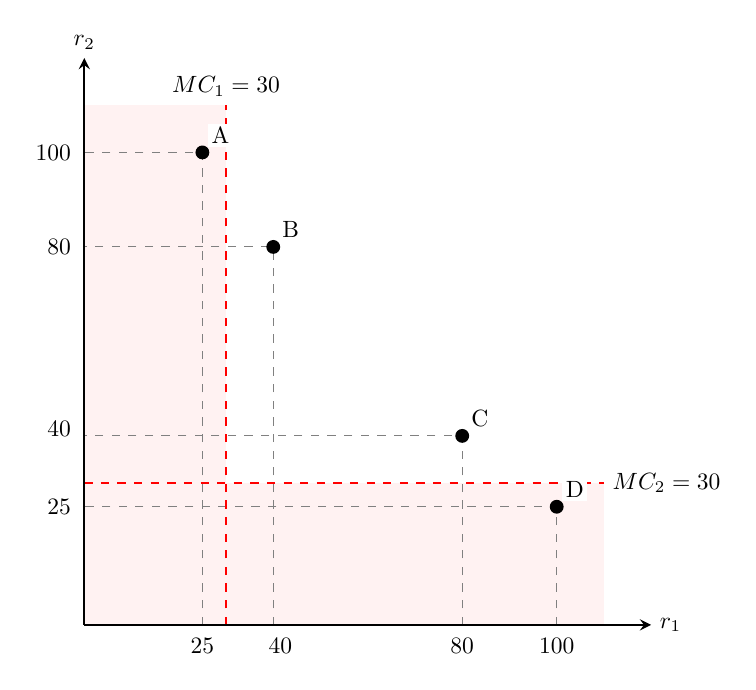
\begin{tikzpicture}[x=0.06cm, y=0.06cm, >=stealth, thick, every node/.style={scale=0.85}]
				% 低效交易区域填充 (红)
				\fill[red!5] (0,0) rectangle (30, 110);
				\fill[red!5] (0,0) rectangle (110, 30);
				
				% 辅助虚线
				\draw[dashed, gray, thin] (25, 0) -- (25, 100) -- (0, 100);
				\draw[dashed, gray, thin] (40, 0) -- (40, 80) -- (0, 80);
				\draw[dashed, gray, thin] (80, 0) -- (80, 40) -- (0, 40);
				\draw[dashed, gray, thin] (100, 0) -- (100, 25) -- (0, 25);
				
				% 边际成本线
				\draw[dashed, red, thick] (30, 0) -- (30, 110) node[above, black] {$MC_1=30$};
				\draw[dashed, red, thick] (0, 30) -- (110, 30) node[right, black] {$MC_2=30$};
				
				% 坐标轴
				\draw[->] (0,0) -- (120,0) node[right] {$r_1$};
				\draw[->] (0,0) -- (0,120) node[above] {$r_2$};
				
				% 轴标签物理分离防重叠
				\node[below, yshift=-2pt] at (25, 0) {25};
				\node[below, xshift=3pt, yshift=-2pt] at (40, 0) {40};
				\node[below, yshift=-2pt] at (80, 0) {80};
				\node[below, yshift=-2pt] at (100, 0) {100};
				
				\node[left, xshift=-2pt] at (0, 25) {25};
				\node[left, yshift=3pt, xshift=-2pt] at (0, 40) {40};
				\node[left, xshift=-2pt] at (0, 80) {80};
				\node[left, xshift=-2pt] at (0, 100) {100};
				
				% 绘制散点
				\fill[black] (25, 100) circle (2.5pt) node[fill=white, inner sep=1.5pt, above right, xshift=2pt, yshift=2pt] {A};
				\fill[black] (40, 80) circle (2.5pt) node[fill=white, inner sep=1.5pt, above right, xshift=2pt, yshift=2pt] {B};
				\fill[black] (80, 40) circle (2.5pt) node[fill=white, inner sep=1.5pt, above right, xshift=2pt, yshift=2pt] {C};
				\fill[black] (100, 25) circle (2.5pt) node[fill=white, inner sep=1.5pt, above right, xshift=2pt, yshift=2pt] {D};
			\end{tikzpicture}
		\end{center}
		\newpage
		
		\item \textbf{一家有线电视公司，除基本服务外，还提供两种产品：体育频道（产品 1）和电影频道（产品 2）。基本服务的用户可以分别订购这两种附加服务，每月各自收取价格 $P_1$ 和 $P_2$，或者可以按价格 $P_B$ 购买两种产品的混合捆绑销售，且 $P_B < P_1 + P_2$。附加服务的边际成本为 0。公司估计出的代表性顾客保留价格分布如图所示。\\
			（1）I、II、III、IV 区的消费者会购买何种产品？请略作解释。\\
			（2）如图所示，保留价格负相关。为什么你认为消费者对频道的保留价格是负相关的？\\
			（3）公司副总裁认为：“因为边际成本为零，混合捆绑销售不比纯捆绑销售更有优势。仅提供纯捆绑销售同样可获高额利润。”你是否同意？\\
			（4）根据图中分布，有线公司是否应该改变目前的定价？该如何改变？}
		
		\textbf{答：}
		基于消费者效用最大化原则，市场需求被个体理性约束（IR）与激励相容约束（IC）划分为四个区域：
		\[
		\begin{aligned}
			\text{区域 I (不购买)} &: r_1 < P_1, \; r_2 < P_2, \; r_1 + r_2 < P_B \\
			\text{区域 II (仅买 1)} &: r_1 \ge P_1, \; r_2 < P_B - P_1 \\
			\text{区域 III (仅买 2)} &: r_2 \ge P_2, \; r_1 < P_B - P_2 \\
			\text{区域 IV (买捆绑)} &: r_1 + r_2 \ge P_B, \; r_1 \ge P_B - P_2, \; r_2 \ge P_B - P_1
		\end{aligned}
		\]
		区域 I 的消费者对单品及组合的保留价格均低于对应售价；区域 II 和 III 的消费者具有极端的单品偏好，购买单品可获得最大消费者剩余；区域 IV 的消费者综合保留价格较高，满足购买捆绑包的激励相容约束。
		
		图中需求散点呈左上至右下聚集，验证了保留价格的负相关性。这深刻反映了电视节目的“闲暇时间约束”：消费者的总闲暇时间是固定的，狂热偏好体育频道的消费者通常无暇高频观看电影频道，反之亦然。
		
		不同意副总裁的观点。纯捆绑策略仅设定单一的 $P_B$，会迫使区域 II 和 III 中原本能带来单品利润的极端偏好者退出市场（因其对组合的估值 $r_1+r_2 < P_B$）。混合捆绑通过单独设定 $P_1$ 与 $P_2$，成功提取了这部分极端偏好者的剩余，其垄断利润严格优于纯捆绑。
		
		公司应当适度提价。观察几何分布可知，现有的定价边界（实线）与实际需求散点之间存在明显的“结构性留白”。这表明在当前价格下，边际消费者的需求完全缺乏弹性。公司可微调提高 $P_1, P_2$ 和 $P_B$，在涨幅触及散点群之前，能无损地将这部分未被触及的剩余转化为利润，且不会流失任何现有顾客。
		
		\begin{center}
			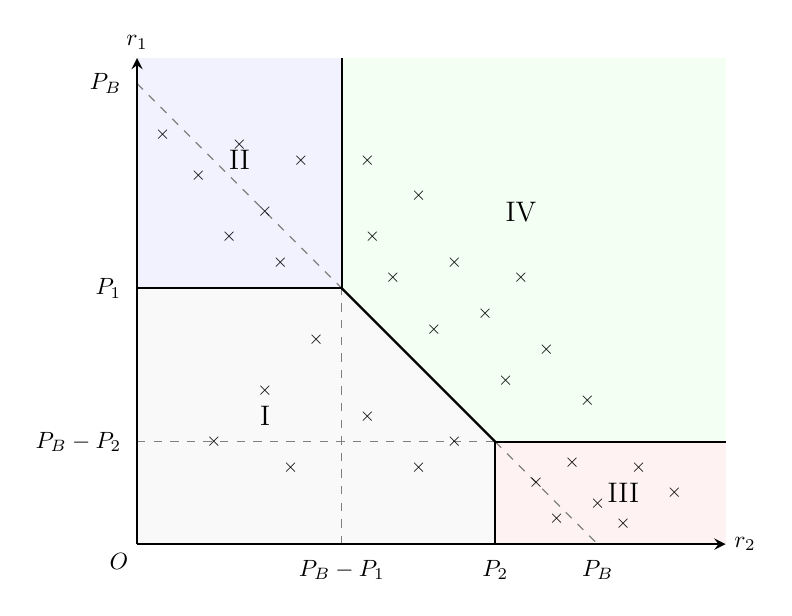
\begin{tikzpicture}[x=0.65cm, y=0.65cm, >=stealth, thick, every node/.style={scale=0.85}]
				% 1. 透明区域填充
				\fill[gray!5] (0,0) -- (7,0) -- (7,2) -- (4,5) -- (0,5) -- cycle; 
				\fill[blue!5] (0,5) rectangle (4,9.5); 
				\fill[red!5] (7,0) rectangle (11.5,2); 
				\fill[green!5] (4,9.5) -- (4,5) -- (7,2) -- (11.5,2) -- (11.5,9.5) -- cycle; 
				
				% 2. 辅助虚线
				\draw[dashed, gray, thin] (4,0) -- (4,5);
				\draw[dashed, gray, thin] (0,2) -- (7,2);
				\draw[dashed, gray, thin] (0,9) -- (4,5); 
				\draw[dashed, gray, thin] (7,2) -- (9,0); 
				
				% 3. 坐标轴与标签
				\draw[->] (0,0) node[below left] {$O$} -- (11.5,0) node[right] {$r_2$};
				\draw[->] (0,0) -- (0,9.5) node[above] {$r_1$};
				
				\node[below, yshift=-3pt] at (4,0) {$P_B-P_1$};
				\node[below, yshift=-3pt] at (7,0) {$P_2$};
				\node[below, yshift=-3pt] at (9,0) {$P_B$};
				
				\node[left, xshift=-3pt] at (0,2) {$P_B-P_2$};
				\node[left, xshift=-3pt] at (0,5) {$P_1$};
				\node[left, xshift=-3pt] at (0,9) {$P_B$};
				
				% 4. 定价分界实线
				\draw (0,5) -- (4,5) -- (4,9.5);
				\draw (4,5) -- (7,2);
				\draw (7,0) -- (7,2) -- (11.5,2);
				
				% 5. 区域标号与留白散点
				\node[font=\large] at (2.5, 2.5) {I};
				\node[font=\large] at (2, 7.5) {II};
				\node[font=\large] at (9.5, 1) {III};
				\node[font=\large] at (7.5, 6.5) {IV};
				
				\begin{scope}[every node/.style={scale=0.7, text=black}]
					\foreach \x/\y in {1.5/2.0, 2.5/3.0, 3.0/1.5, 3.5/4.0, 4.5/2.5, 5.5/1.5, 6.2/2.0} { \node at (\x,\y) {$\times$}; }
					\foreach \x/\y in {0.5/8.0, 1.2/7.2, 2.0/7.8, 2.5/6.5, 3.2/7.5, 1.8/6.0, 2.8/5.5} { \node at (\x,\y) {$\times$}; }
					\foreach \x/\y in {7.8/1.2, 8.5/1.6, 9.0/0.8, 9.8/1.5, 10.5/1.0, 8.2/0.5, 9.5/0.4} { \node at (\x,\y) {$\times$}; }
					\foreach \x/\y in {4.6/6.0, 5.0/5.2, 5.5/6.8, 6.2/5.5, 6.8/4.5, 7.5/5.2, 8.0/3.8, 8.8/2.8, 4.5/7.5, 5.8/4.2, 7.2/3.2} { \node at (\x,\y) {$\times$}; }
				\end{scope}
			\end{tikzpicture}
		\end{center}
		\newpage
		
		\item \textbf{一个有垄断势力的厂商，面临的需求曲线为 $P = 100 - 3Q + 4A^{1/2}$，总成本函数为 $C = 4Q^2 + 10Q + A$，其中 $A$ 是广告支出水平；$P$ 和 $Q$ 分别是价格和产量。（1）找出实现厂商利润最大化的 $A$、$Q$ 和 $P$ 的值。（2）计算该厂商在它的利润最大化的 $A$、$Q$ 和 $P$ 水平下，垄断势力的勒纳指数 $L = \frac{P - MC}{P}$ 的值。}
		
		\textbf{答：}
		（1）厂商通过同时选择最优产量 $Q$ 与广告投入 $A$ 来实现利润最大化。根据需求函数与总成本函数，可构建利润目标函数：
		\[
		\begin{aligned}
			\pi(Q, A) &= P \cdot Q - C \\
			&= (100 - 3Q + 4A^{1/2})Q - (4Q^2 + 10Q + A) \\
			&= -7Q^2 + 90Q + 4QA^{1/2} - A
		\end{aligned}
		\]
		利润最大化要求利润函数对 $Q$ 和 $A$ 的一阶偏导数同时为零，即满足以下一阶条件：
		\[
		\begin{aligned}
			\frac{\partial \pi}{\partial Q} &= 90 - 14Q + 4A^{1/2} = 0 \\
			\frac{\partial \pi}{\partial A} &= 2QA^{-1/2} - 1 = 0
		\end{aligned}
		\]
		由关于广告 $A$ 的一阶条件可推得 $A^{1/2} = 2Q$。将其代入关于产量 $Q$ 的一阶条件中，消去 $A$ 以求解最优产量：
		\[
		\begin{aligned}
			90 - 14Q + 4(2Q) = 0 \implies 6Q = 90
		\end{aligned}
		\]
		解得最优产量 $Q = 15$。将其回代可得最优广告支出 $A = (2 \times 15)^2 = 900$。此时，将 $Q$ 与 $A$ 的均衡值代入反需求函数，求得利润最大化定价：
		\[
		\begin{aligned}
			P = 100 - 3 \times 15 + 4 \times 30 = 175
		\end{aligned}
		\]
		
		（2）在利润最大化产量 $Q=15$ 处，厂商的边际成本为总成本函数对产量的导数：
		\[
		\begin{aligned}
			MC = \frac{\partial C}{\partial Q} = 8Q + 10 = 8 \times 15 + 10 = 130
		\end{aligned}
		\]
		根据勒纳指数公式，测度该垄断厂商的市场势力：
		\[
		\begin{aligned}
			L = \frac{P - MC}{P} = \frac{175 - 130}{175} = \frac{45}{175} \approx 0.257
		\end{aligned}
		\]
		该勒纳指数表明，在最优广告投入的加持下，厂商的最优定价高出其边际成本约 $25.7\%$，反映了其通过广告塑造差异化并成功获取的市场加成能力。
	\end{enumerate}
	\newpage
	\section{第11章附录：纵向联合厂商}
	\begin{enumerate}[label=\textbf{\arabic*.}, leftmargin=*]
		\item \textbf{假设波音公司 787 飞机的每月销量面对以下需求函数：$$Q = 120 - 0.5P$$其中 $Q$ 是每月出售的飞机数量，$P$ 是价格（单位：百万美元）。每架飞机使用通用电气公司生产的一套发动机，波音为每套发动机支付 $P_E$ 的价钱。通用电气公司生产一套发动机的边际成本是 20 百万美元。除了支付发动机的费用外，波音公司还有一个每架飞机 100 百万美元的边际成本。\\（1）在独立决策条件下，各方的利润最大化定价是多少？\\（2）若两家公司纵向一体化，飞机的价格又是多少？}
		
		\textbf{答：}
		在独立决策即双重边际化状态下，两家厂商各自追求自身利润最大化。由飞机需求函数可得飞机的反需求函数为 $P = 240 - 2Q$。下游波音公司的边际收益为 $MR_B = 240 - 4Q$。给定发动机价格 $P_E$，波音公司的总边际成本为 $100 + P_E$。由利润最大化条件 $MR_B = MC$ 可得：
		\[
		\begin{aligned}
			240 - 4Q = 100 + P_E \implies P_E = 140 - 4Q
		\end{aligned}
		\]
		此式即为上游通用电气公司所面临的引致需求函数。通用电气据此确立自身的边际收益为 $MR_E = 140 - 8Q$，结合其发动机边际成本 $MC_E = 20$，由 $MR_E = MC_E$ 解得每月最优均衡产量 $Q = 15$。将产量倒推回各级定价公式，最终得到发动机的价格 $P_E = 80$ 百万美元，飞机的最终零售价格为 $P = 210$ 百万美元。
		
		若波音公司收购通用电气发动机部门实现纵向一体化，两阶段博弈便转化为单阶段的联合利润最大化问题。此时发动机的内部中间转让不再谋求中间加成，企业的合并边际成本直接表现为两阶段生产成本的简单叠加：
		\[
		\begin{aligned}
			MC = MC_E + MC_B' = 20 + 100 = 120
		\end{aligned}
		\]
		一体化企业的整体边际收益函数仍为 $MR = 240 - 4Q$。由整体最优决策条件 $MR = MC$ 联立方程：
		\[
		\begin{aligned}
			240 - 4Q = 120 \implies Q = 30
		\end{aligned}
		\]
		解得一体化后的每月最优飞机产量为 30 架，对应的飞机市场零售价格降至 $P = 180$ 百万美元。对比可知，纵向一体化有效消除了中间加成带来的多重效率损失，实现了产量扩大与终端价格下降的双重福利改善。
		
		\begin{center}
			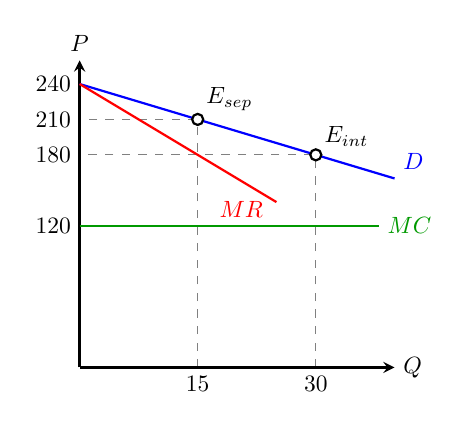
\begin{tikzpicture}[x=0.1cm, y=0.015cm, >=stealth, thick, every node/.style={scale=0.85}]
				% 1. 辅助虚线
				\draw[dashed, gray, thin] (15,0) -- (15,210) -- (0,210);
				\draw[dashed, gray, thin] (30,0) -- (30,180) -- (0,180);
				\draw[dashed, gray, thin] (0,120) -- (35,120);
				% 2. 坐标轴
				\draw[->] (0,0) -- (40,0) node[right] {$Q$};
				\draw[->] (0,0) -- (0,260) node[above] {$P$};
				% 3. 供需实线
				\draw[thick, blue, domain=0:40] plot (\x, {240 - 2*\x}) node[above right] {$D$};
				\draw[thick, red, domain=0:25] plot (\x, {240 - 4*\x}) node[below left,yshift=4pt,xshift=-2pt] {$MR$};
				\draw[thick, green!60!black] (0,120) -- (38,120) node[right] {$MC$};
				% 4. 均衡点
				\fill[draw=black, fill=white] (15,210) circle (2pt) node[above right] {$E_{\text{sep}}$};
				\fill[draw=black, fill=white] (30,180) circle (2pt) node[above right] {$E_{\text{int}}$};
				% 5. 坐标标签
				\node[below] at (15,0) {$15$};
				\node[below] at (30,0) {$30$};
				\node[left] at (0,120) {$120$};
				\node[left] at (0,180) {$180$};
				\node[left] at (0,210) {$210$};
				\node[left] at (0,240) {$240$};
			\end{tikzpicture}
		\end{center}
		\newpage
		\item \textbf{回顾莱斯卡摩托赛车公司的数字例子。计算在如下三种情况下上游分部、下游分部和厂商总体所赚到的利润：（a）没有发动机的竞争性外部市场；（b）有一个市场价格为 6000 美元的发动机的竞争性外部市场；（c）该厂商是发动机外部市场的垄断供应商。并进行利润分布的比较分析。}
		
		\textbf{答：}
		根据已知条件，摩托车市场反需求函数为 $P = 20000 - Q$，下游组装边际成本 $MC_D = 8000$，上游发动机边际成本 $MC_E = 4000 + Q_E$。
		
		在没有发动机外部市场的情形下，内部转移定价需满足下游的净边际收益等于上游的边际成本，即 $MR_{\text{net}} = MR - MC_D = MC_E$。
		\[
		\begin{aligned}
			(20000 - 2Q) - 8000 = 4000 + Q \implies 3Q = 8000 \implies Q \approx 2666.67
		\end{aligned}
		\]
		解得均衡产量后，代入各分部利润函数计算可得，公司总利润约为 1066.67 万美元。
		
		当存在一个竞争性外部市场且发动机价格固定为 $P_E = 6000$ 美元时，市场价格构成了内部转让的最高机会成本。下游组装部门按照 $MR = MC_D + P_E$ 决定最终起运产量：
		\[
		\begin{aligned}
			20000 - 2Q = 8000 + 6000 \implies 2Q = 6000 \implies Q = 3000
		\end{aligned}
		\]
		此时，上游分部根据外部市场价决定自身产量，由 $MC_E = 4000 + Q_E = 6000$ 解得 $Q_E = 2000$。缺口的 1000 台发动机由下游直接从外部市场外购。在此配置下，公司总利润提升至 1100 万美元。
		
		当上游分部成为外部发动机市场的垄断供应商时，上游同时面对内部和外部两个独立的引致需求。最优决策要求内部净边际收益、外部边际收益与上游边际成本三者完全相等，即 $MR_{\text{net}} = MR_{\text{ext}} = MC_E$。联立各分部最优化一阶方程，可精确解得内部摩托车产量 $Q_D = 2250$，外部发动机销量 $Q_E = 1250$。此时上游总产量为 3500，公司合并总利润达到最大值 1275 万美元。
		
		\begin{center}
			\small
			\renewcommand{\arraystretch}{1.3}
			\setlength{\tabcolsep}{4pt}
			\begin{tabular}{|l|c|c|c|}
				\hline
				\textbf{市场运行体制} & \textbf{上游分部利润} & \textbf{下游分部利润} & \textbf{公司总利润} \\
				\hline
				(a) 无外部市场 & 355.56 & 711.11 & 1066.67 \\
				(b) 竞争性外部市场 & 200.00 & 900.00 & 1100.00 \\
				(c) 外部垄断供应商 & 768.75 & 506.25 & 1275.00 \\
				\hline
			\end{tabular}
		\end{center}
		综上比较可知，若从母公司总体利润及上游分部利润来看，情况 (c) 带来的收益最高；而对于下游组装分部而言，情况 (b) 提供的廉价外部竞争价源使其能够赚取最多的剩余。
		\newpage
		\item \textbf{阿贾克斯计算机公司制造一种用于办公楼气温控制的计算机。该公司使用其上游分部生产的一种微处理器，微处理器以常数边际成本 500 美元生产，下游分部装配计算机的边际成本为常数 700 美元。公司最初以 2000 美元价格垄断销售计算机且无外部市场。（1）若微处理器外部垄断市场发展起来且售价 1000 美元（需求无关联），内部转移价格与计算机产量如何变化？（2）若两市场需求具有竞争替代性，上述回答如何变化？}
		
		\textbf{答：}
		在初始无外部市场且下游存在管理定价偏误时，原产量由于中间加成被抑制在较低水平。在第一种情形下，虽然外部微处理器市场发展起来且上游具备 1000 美元的垄断势力，但由于微处理器与最终计算机在消费需求上完全独立，外部市场的开辟并不会改变内部资源配置的边际条件。
		
		为了实现母公司整体利润最大化，对于内部下游分部而言，微处理器的名义机会成本依然等于其生产的真实边际成本。因此，最优内部转移价格应当坚定地维持在 $P_T = MC_E = 500$ 美元。
		\[
		\begin{aligned}
			MR_{\text{net}} = (2000 - 2Q_D) - 700 = 500 \implies Q_D = 400
		\end{aligned}
		\]
		解得内部计算机产量增加至 400 台，终端售价降至 1600 美元。上游分部同时对外部市场实施垄断定价，由外部边际收益等于边际成本（$1000 - 2Q_E = 500$）解得外部出货量 $Q_E = 250$ 个。转移价格向边际成本的回归有效释放了下游的生产约束。
		
		在第二种情形下，如果计算机与微处理器在最终消费上具有竞争替代性，上游向外部出售微处理器会直接分流下游计算机的需求。此时，内部使用微处理器的机会成本不再是单纯的生产成本，而是被迫放弃的外部边际收益。上游在外部的最优边际收益为 $MR_{\text{ext}} = 750$ 美元。为了修正跨部门的负外部性，最优内部转移价格必须同步上调至 $P_T = 750$ 美元。下游分部面对上升的内部转让价格，其核算边际成本抬高，导致最终计算机产量被克制在 200 台的水平，以此避免内部双市场间的恶性串谋。
		
		\begin{center}
			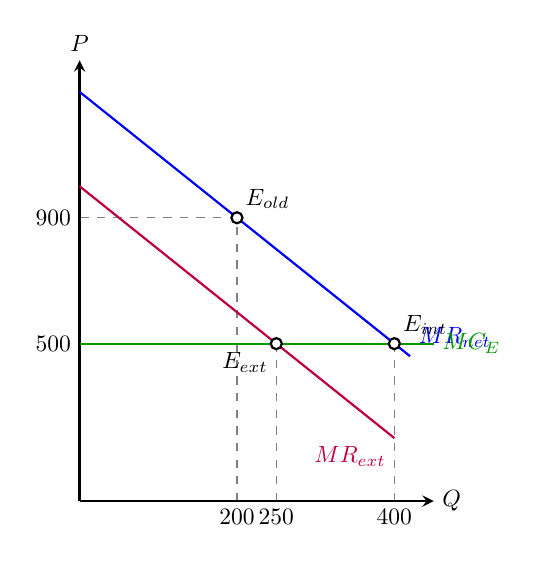
\begin{tikzpicture}[x=0.01cm, y=0.004cm, >=stealth, thick, every node/.style={scale=0.85}]
				% 1. 辅助虚线
				\draw[dashed, gray, thin] (200,0) -- (200,900) -- (0,900);
				\draw[dashed, gray, thin] (400,0) -- (400,500);
				\draw[dashed, gray, thin] (250,0) -- (250,500);
				\draw[dashed, gray, thin] (0,500) -- (450,500);
				% 2. 坐标轴
				\draw[->] (0,0) -- (450,0) node[right] {$Q$};
				\draw[->] (0,0) -- (0,1400) node[above] {$P$};
				% 3. 曲线绘制
				\draw[thick, blue, domain=0:420] plot (\x, {1300 - 2*\x}) node[above right] {$MR_{\text{net}}$};
				\draw[thick, purple, domain=0:400] plot (\x, {1000 - 2*\x}) node[below left] {$MR_{\text{ext}}$};
				\draw[thick, green!60!black] (0,500) -- (450,500) node[right] {$MC_E$};
				% 4. 均衡交点
				\fill[draw=black, fill=white] (200,900) circle (2pt) node[above right] {$E_{\text{old}}$};
				\fill[draw=black, fill=white] (400,500) circle (2pt) node[above right] {$E_{\text{int}}$};
				\fill[draw=black, fill=white] (250,500) circle (2pt) node[below left] {$E_{\text{ext}}$};
				% 5. 坐标标签
				\node[below] at (200,0) {$200$};
				\node[below] at (250,0) {$250$};
				\node[below] at (400,0) {$400$};
				\node[left] at (0,500) {$500$};
				\node[left] at (0,900) {$900$};
			\end{tikzpicture}
		\end{center}
		\newpage
		\item \textbf{锐步生产和销售跑鞋，最终市场需求为 $P = 11 - 1.5Q_S$。生产一双鞋需要一平方码皮革。上游成本函数为 $TC_S = 2Q_S$，下游制鞋成本为 $TC_C = 1 + Q_C + 0.5Q_C^2$。试求解：（1）非一体化独立决策下的内部转移价格与产量；（2）若外在皮革市场竞争价为 1.5 美元，企业的最优内外供求配置；（3）若上游垄断外部皮革市场且面对需求 $P = 32 - Q_S$，最优内部转移价格与外部售价。}
		
		\textbf{答：}
		在无外部市场的纵向独立决策（分立博弈）下，下游的净边际收益函数表现为 $MR_{\text{net}} = MR - MC_C = (11 - 3Q_C) - (1 + Q_C) = 10 - 4Q_C$。上游分部将此视为自身的引致需求曲线，并通过使自身边际收益等于边际成本（$10 - 8Q_S = 2$）来实施加成定价。解得双方在内部非集成状态下的均衡产量 $Q_S = Q_C = 1$。此时，上游开出的内部转移价格固定在 $P_T = 10 - 4(1) = 6$ 美元。
		
		当引入一竞争性外部市场且皮革价格低至 $P_F = 1.5$ 美元时，由于上游自身成形皮革的常数边际成本 $MC_S = 2$ 严格大于外部市场价，母公司理性的策略是命令上游分部完全关停成形生产线，即上游产量 $Q_S = 0$。下游制鞋分部转而全额跨期外购廉价皮革，此时下游面对的最优转移买入价等价于市场价 $P_T = 1.5$ 美元。下游总核算边际成本下降为 $MC_{\text{total}} = (1 + Q_C) + 1.5 = 2.5 + Q_C$。联立下游边际收益方程：
		\[
		\begin{aligned}
			11 - 3Q_C = 2.5 + Q_C \implies 4Q_C = 8.5 \implies Q_C = 2.125
		\end{aligned}
		\]
		解得最终跑鞋产量扩张至 2.125 双，所需 2.125 平方码皮革全部由外部市场输入。
		
		当上游分部成功转型为外部高质量皮革市场的垄断供应商时，上游再次拥有了对内外两个市场的统筹定价权。为了最大化母公司利润，其资源配置逻辑要求内部净边际收益与外部边际收益共同锚定在上游的真实生产边际成本上，即 $MR_{\text{net}} = MR_{\text{ext}} = MC_S = 2$。
		
		对于内部下游，联立方程 $10 - 4Q_C = 2$ 解得最优制鞋产量 $Q_C = 2$ 双，此时对应的内部最优化转移价格应直接退回其生产边际成本 $P_T = 2$ 美元。
		
		对于外部市场，联立方程 $MR_{\text{ext}} = 32 - 2Q_E = 2$ 解得向外部市场倾销的皮革数量 $Q_E = 15$ 平方码，代入外部需求函数得到外部零售价 $P_E = 17$ 美元。
		
		\begin{center}
			\small
			\renewcommand{\arraystretch}{1.3}
			\setlength{\tabcolsep}{4pt}
			\begin{tabular}{|l|c|c|c|}
				\hline
				\textbf{生产与市场核算指标} & \textbf{(a) 无外部市场(分立)} & \textbf{(b) 竞争性外部市场} & \textbf{(c) 外部垄断市场} \\
				\hline
				上游皮革产量（平方码） & 1 & 0 & 17 \\
				下游跑鞋产量（双） & 1 & 2.125 & 2 \\
				内部转移/外购价（美元） & 6 & 1.5 & 2 \\
				外部皮革售价（美元） & - & 1.5 & 17 \\
				\hline
			\end{tabular}
		\end{center}
	\end{enumerate}
	% =======================================================
	%                 第 12 章：垄断竞争与寡头垄断
	% =======================================================
	\chapter{垄断竞争与寡头垄断}
	
	\section{复习题}
	\begin{enumerate}[label=\textbf{\arabic*.}, leftmargin=*]
		\item \textbf{垄断竞争市场的特征是什么？在这样一个市场中，如果一厂商推出一种新型的、改进的产品，对均衡价格和产量会产生什么影响？}
		
		\textbf{答：}
		垄断竞争市场具有两个核心特征。一是集团内存在大量厂商生产具有差别但高度可替代的同类产品，这使得厂商对自身品牌产品具有一定的垄断定价权，同时又面临激烈的市场竞争；二是市场不存在实质性的进入或退出壁垒，厂商在长期中可以自由进出该行业。
		
		当某一厂商推出新型且改进的产品时，该厂商通过增强产品差异化成功提升了自身的垄断优势。在短期内，该创新厂商面临的需求曲线向外平移且变得更缺乏弹性，从而导致其自身的均衡价格和产量同时上升，并能够获取超额利润。然而，这一创新举措会蚕食其他竞争对手的市场份额，导致其他厂商所面临的需求曲线向内平移，其余厂商的均衡价格和产量随之下降。在长期中，由于不存在进入壁垒，大批模仿者会受利益驱动进入并推出相似品牌，这将使得创新厂商的超额利润逐渐消失，直至市场达到新的长期均衡。
		
		\item \textbf{为什么在垄断竞争中厂商的需求曲线比总的市场需求曲线要平坦？假设一家垄断竞争厂商短期中有一个利润，长期中它的需求曲线会发生什么变化？}
		
		\textbf{答：}
		在垄断竞争市场中，单个厂商的需求曲线表示消费者对该特定品牌商品的需求。由于不同品牌之间具有极高的替代性，消费者对价格变动高度敏感，因此单个厂商的需求曲线具有较高的价格弹性，在图形上表现得较为平坦。相反，总的市场需求曲线代表消费者对整个行业大类产品的总需求，这类产品由于缺乏行业外的紧密替代品，其整体需求弹性显著小于单个品牌的需求弹性，因而市场需求曲线更为陡峭。
		
		如果一家垄断竞争厂商在短期内获得经济利润，这种超额利润将吸引新的厂商携带相互竞争的新品牌进入市场。在市场总需求规模不变的前提下，新厂商的加入会分流原有厂商的客户，导致原有厂商的市场份额缩减。原有厂商面临的需求曲线 $D_{SR}$ 将持续向内平移，并伴随替代品数量的增加而变得更加富有弹性。这一调整过程一直持续到需求曲线平移至与长期平均成本曲线 $ATC$ 恰好相切的位置 $D_{LR}$。此时，边际收益曲线 $MR_{LR}$ 与边际成本曲线 $MC$ 交于均衡产量 $Q_{LR}$，厂商的超额利润彻底消失，实现长期均衡。
		\[
		\begin{aligned}
			MR_{LR}(Q_{LR}) &= MC(Q_{LR}) \\
			P_{LR} = D_{LR}(Q_{LR}) &= ATC(Q_{LR})
		\end{aligned}
		\]
		
		\begin{center}
			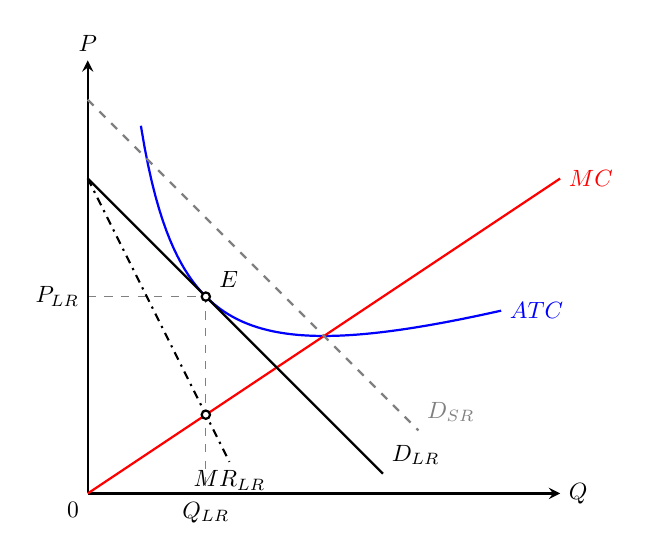
\begin{tikzpicture}[x=1.5cm, y=0.5cm, >=stealth, thick, every node/.style={scale=0.85}]
				% 1. 全局辅助虚线 (最底层)
				\draw[dashed, gray, thin] (0,5) -- (1,5) -- (1,0);
				
				% 2. 坐标轴与防重叠标签
				\draw[->] (0,0) -- (4,0) node[right] {$Q$};
				\draw[->] (0,0) -- (0,11) node[above] {$P$};
				\node[below left] at (0,0) {$0$};
				\node[below] at (1,0) {$Q_{LR}$};
				\node[left] at (0,5) {$P_{LR}$};
				
				% 3. 供需实线与成本曲线 (严格裁切domain)
				\draw[domain=0.45:3.5, samples=100, color=blue] plot (\x, {4/\x + \x}) node[right] {$ATC$};
				\draw[domain=0:4, samples=50, color=red] plot (\x, {2*\x}) node[right] {$MC$};
				\draw[domain=0:2.8, color=gray, dashed] plot (\x, {10 - 3*\x}) node[above right] {$D_{SR}$};
				\draw[domain=0:2.5, color=black] plot (\x, {8 - 3*\x}) node[above right] {$D_{LR}$};
				\draw[domain=0:1.2, color=black, dashdotted] plot (\x, {8 - 6*\x}) node[below] {$MR_{LR}$};
				
				% 4. 均衡点与标号 (清除交叉线干扰)
				\filldraw[fill=white, draw=black] (1,5) circle (1.5pt) node[above right, xshift=2pt] {$E$};
				\filldraw[fill=white, draw=black] (1,2) circle (1.5pt);
			\end{tikzpicture}
		\end{center}
		
		\item \textbf{有些专家论证说市场上早餐麦片的品牌太多了。给出一个支持该观点的论证。给出一个反对该观点的论证。}
		
		\textbf{答：}
		支持品牌过多的论证立足于经济效率与资源配置视角。由于早餐麦片市场属于典型的垄断竞争结构，厂商上面临向右下方倾斜的需求曲线，这导致长期均衡时厂商只能在平均成本曲线向右下方倾斜的阶段进行生产。这意味着行业内存在显著的过剩生产能力，即实际产量未能达到长期平均成本最低的最优生产规模。众多品牌恶意瓜分了有限的市场总需求，使得每家厂商都无法充分实现规模经济，从而造成了社会资源的低效配置与重复浪费。
		
		反对品牌过多的论证则立足于消费者福利与产品多样性视角。虽然垄断竞争结构导致了一定程度的无谓损失与过剩生产能力，但由于各品牌之间的替代性极强，单个厂商所拥有的实际垄断势力极为有限，由垄断势力引起的非效率成本在现实中微乎其微。相反，早餐麦片的不同品牌在口味、营养成分、包装设计及目标群体上各具特色，极大满足了消费者多元化的异质性偏好。产品多样化所带来的巨大消费者剩余与心理满足感，往往远超由需求曲线倾斜所引发的微小效率损失。
		
		\item \textbf{为什么古诺均衡是稳定的（即为什么一旦均衡，各厂商就不会有改变它们产量水平的冲动）？即使它们被允许公开共谋，它们为什么不将产量定在共同利润最大化的水平（即如果它们共谋时会选择的水平）？}
		
		\textbf{答：}
		古诺均衡的稳定性源于其本质上是一个纳什均衡。在古诺博弈中，每个寡头厂商都是在将竞争对手的产量视为固定的前提下，最大化自身的个体利润。一旦市场达到古诺均衡点，每家厂商所选择的产量恰好是对邻近对手实际产量的最优反应。此时，在给定对方策略既定的约束下，没有任何一家厂商能够通过单方面调整自身的产量来获得更多利润，因而各厂商均缺乏改变现状的内在冲动，市场达成稳态。
		
		即使法律或规则允许厂商公开进行共谋，共同利润最大化的联合垄断产出水平也是极不稳定的。由于缺乏外部强制执行机制，共谋契约面临着根深蒂固的“囚徒困境”。对任何一家厂商而言，在对方严格遵守低产高价的共谋协议时，自身单方面偷偷增加产量、实施欺诈，总是能够凭借高价格和高份额获得更庞大的个体经济利润。这种理性背叛的占优策略激励使得每个厂商都有扩产的冲动，最终导致共谋协议彻底瓦解，产量重新回落至非合作的古诺均衡水平。
		\newpage
		\item \textbf{在斯塔克博格模型中，先决定产量的厂商有一种优势。解释为什么？}
		
		\textbf{答：}
		斯塔克博格模型属于序贯产量博弈。先动厂商 1 的优势在于，它能够将后动厂商 2 的反应函数 $R_2$ 视为已知约束，并直接内生化到自身的利润最大化决策中：
		\[
		\begin{aligned}
			\max_{Q_1} \quad &\pi_1 = P(Q_1 + Q_2) \cdot Q_1 - TC_1(Q_1) \\
			\text{s.t.} \quad &Q_2 = R_2(Q_1)
		\end{aligned}
		\]
		
		这种序贯决策改变了博弈的均衡位置。如图所示，若两厂商同时决策，市场均衡点位于两条反应曲线 $R_1$ 与 $R_2$ 的交点，即古诺均衡点 $C(Q_1^C, Q_2^C)$。而在序贯博弈中，由于厂商 1 率先决策，博弈均衡点将沿着厂商 2 的反应曲线 $R_2$ 向右下方平移，最终确定在斯塔克博格均衡点 $S(Q_1^S, Q_2^{M,S})$。
		
		此时，由于厂商 1 抢先确立了较高的产量 $Q_1^S$，理性的厂商 2 只能接受这一既定事实。为了在剩余的市场空间中最大化自身利润，厂商 2 必须在其反应曲线 $R_2$ 上选择较低的产量 $Q_2^{M,S}$（在线性需求下，该产量恰好等于双方在共谋点 $M$ 时厂商 2 的分配产量 $Q_2^M$）。最终，厂商 1 凭借决策的时序优势，获得了更大的市场份额与更高的利润。
		
		\begin{center}
			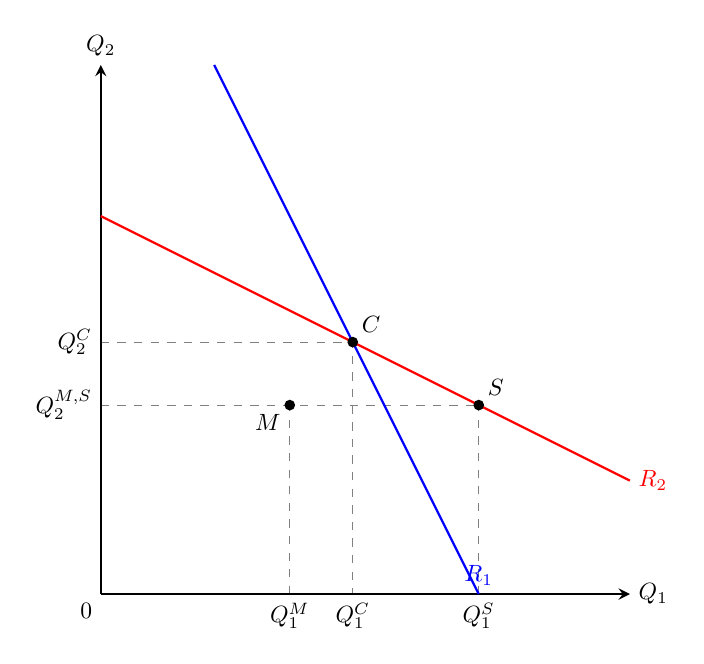
\begin{tikzpicture}[x=1.6cm, y=1.6cm, >=stealth, thick, every node/.style={scale=0.85}]
				% 1. 全局辅助虚线
				\draw[dashed, gray, thin] (0,2) -- (2,2) -- (2,0);
				\draw[dashed, gray, thin] (0,1.5) -- (3,1.5);
				\draw[dashed, gray, thin] (1.5,0) -- (1.5,1.5);
				\draw[dashed, gray, thin] (3,0) -- (3,1.5);
				
				% 2. 坐标轴
				\draw[->] (0,0) -- (4.2,0) node[right] {$Q_1$};
				\draw[->] (0,0) -- (0,4.2) node[above] {$Q_2$};
				\node[below left] at (0,0) {$0$};
				
				% 轴标签物理分离
				\node[below] at (1.5,0) {$Q_1^M$};
				\node[below] at (2,0) {$Q_1^C$};
				\node[below] at (3,0) {$Q_1^S$};
				\node[left] at (0,1.5) {$Q_2^{M,S}$};
				\node[left] at (0,2) {$Q_2^C$};
				
				% 3. 反应曲线
				\draw[domain=0.9:3.0, samples=50, color=blue] plot (\x, {6 - 2*\x}) node[above] {$R_1$};
				\draw[domain=0:4.2, samples=50, color=red] plot (\x, {3 - 0.5*\x}) node[right] {$R_2$};
				
				% 4. 关键决策点标号
				\filldraw[fill=black] (2,2) circle (1.5pt) node[above right, fill=white, inner sep=1.5pt,xshift=2pt,yshift=2pt] {$C$};
				\filldraw[fill=black] (3,1.5) circle (1.5pt) node[above right, fill=white, inner sep=1.5pt,xshift=2pt,yshift=2pt] {$S$};
				\filldraw[fill=black] (1.5,1.5) circle (1.5pt) node[below left, fill=white, inner sep=1.5pt,xshift=-2pt,yshift=-2pt] {$M$};
			\end{tikzpicture}
		\end{center}
		
		\item \textbf{古诺模型和伯特兰模型的相同之处是什么？两个模型有何区别？}
		
		\textbf{答：}
		古诺模型与伯特兰模型的相同之处在于两者皆属于经典的双寡头非合作博弈模型。在这两个模型中，市场上均只有两家厂商生产同质的产品，且面临完全相同的市场需求结构。同时，厂商在进行单阶段决策时都具有天真的静态预期特征，即将竞争对手的行为变量（无论是产量还是价格）视为固定不变的常数，以此推导自身的反应函数来寻求纳什均衡。
		
		两者的核心区别主要体现在策略变量与经济效应两个维度。在策略变量方面，古诺模型中的厂商以产量为决策变量，通过调节供求总量来间接决定市场出清价格；而伯特兰模型中的厂商则直接以价格为决策变量，通过价格互搏来直接争夺市场份额。在经济效应方面，由于同质品驱动下的恶性价格竞争，伯特兰模型会导致经典的“伯特兰悖论”，即只要两家厂商的边际成本相同，最终的均衡价格就会被一路压低至边际成本水平，厂商利润归零，社会福利达到完全竞争状态下的最优化；而古诺模型的厂商通过控制数量规避了极端价格战，其最终的市场总产量高于垄断水平但低于竞争水平，均衡价格高于边际成本，厂商仍能赚取部分超额利润。
		\newpage
		
		\item \textbf{解释当厂商进行价格竞争时纳什均衡的意义。为什么这种均衡是稳定的？为什么厂商们不将价格提高到最大化它们的共同利润的水平？}
		
		\textbf{答：}
		在同质品的双寡头价格竞争（伯特兰模型）中，纳什均衡的经济学意义在于体现了激烈的边际定价结果。此时，两厂商的最优策略是竞相削价以争夺整个市场，导致最终的纳什均衡价格等于边际成本：
		\[ P_1 = P_2 = MC \]
		
		这种均衡极其稳定，因为任何厂商都缺乏单方面改变价格的冲动。若某一厂商单方面提价，将立即失去所有市场份额，销售量归零；若其单方面降价，价格将低于边际成本，导致每单位生产都面临实质性亏损。因此，没有任何一方能通过偏离该均衡价格而获得更高利润。
		
		厂商无法将价格维持在共同利润最大化的垄断水平，本质上是因为陷入了“囚徒困境”。在共谋价格下，每个厂商都面临着单方面微幅降价以独吞整个市场利润的巨大诱惑。由于缺乏合法的强制信任约束，且此类公开串通行为受到反垄断法的严厉禁止，理性的非合作博弈必然导致共谋协议走向瓦解，价格最终回落至边际成本相等的纳什均衡。
		
		\item \textbf{折弯的需求曲线描述了价格黏性。解释该模型是如何说明问题的。它的局限性是什么？为什么价格黏性在寡头垄断市场产生出来？}
		
		\textbf{答：}
		斯威齐模型通过竞争对手“跟跌不跟涨”的不对称行为假定，解释了寡头垄断市场的价格黏性。如该图所示，主观需求曲线 $D$ 在当前价格 $P^*$ 处发生折弯。当厂商提价时，对手保持价格不变以独立夺取市场，使得提价段需求曲线极具弹性；当厂商降价时，对手出于防御相继跟进降价，使得降价段需求曲线缺乏弹性。
		
		\begin{center}
			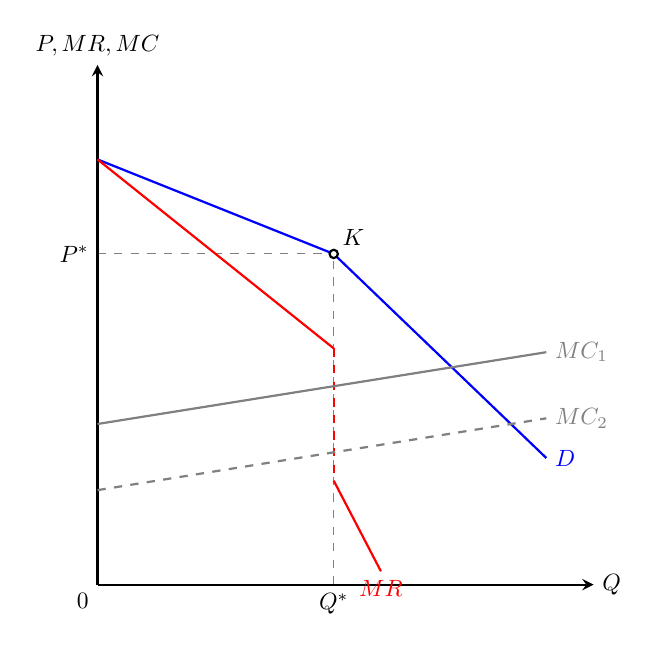
\begin{tikzpicture}[x=1.5cm, y=1.2cm, >=stealth, thick, every node/.style={scale=0.85}]
				% 1. 全局辅助虚线 (最底层)
				\draw[dashed, gray, thin] (0,3.5) -- (2,3.5);
				\draw[dashed, gray, thin] (2,0) -- (2,3.5);
				
				% 2. 坐标轴与标签物理分离 (防重叠)
				\draw[->] (0,0) -- (4.2,0) node[right] {$Q$};
				\draw[->] (0,0) -- (0,5.5) node[above] {$P, MR, MC$};
				\node[below left] at (0,0) {$0$};
				\node[left] at (0,3.5) {$P^*$};
				\node[below] at (2,0) {$Q^*$};
				
				% 3. 供需曲线与边际成本 (严格裁切定义域，确保MR完全在X轴上方)
				\draw[domain=0:2, color=blue] plot (\x, {4.5 - 0.5*\x});
				\draw[domain=2:3.8, color=blue] plot (\x, {5.9 - 1.2*\x}) node[right] {$D$};
				
				\draw[domain=0:2, color=red] plot (\x, {4.5 - \x});
				\draw[dashed, red] (2,2.5) -- (2,1.1); % 垂直间断区间 [1.1, 2.5]
				\draw[domain=2:2.4, color=red] plot (\x, {5.9 - 2.4*\x}) node[below] {$MR$};
				
				\draw[domain=0:3.8, color=gray] plot (\x, {1.7 + 0.2*\x}) node[right] {$MC_1$};
				\draw[domain=0:3.8, color=gray, dashed] plot (\x, {1.0 + 0.2*\x}) node[right] {$MC_2$};
				
				% 4. 关键折弯点标号 (fill=white 消除交叉干扰)
				\filldraw[fill=white, draw=black] (2,3.5) circle (1.5pt) node[above right] {$K$};
			\end{tikzpicture}
		\end{center}
		
		这种几何层面的折弯导致边际收益曲线 $MR$ 在均衡产量 $Q^*$ 处形成一段垂直的间断区间。这意味着，只要厂商的边际成本曲线在 $MC_1$ 与 $MC_2$ 之间的垂直空隙内发生上下波动，其利润最大化（$MR = MC$）的均衡产量仍将牢牢锁定在 $Q^*$，对应的市场价格也将维持在 $P^*$ 不变，从而表现出强烈的价格刚性。
		
		该模型的局限性在于其具有外生性，它只能在已知一个既定价格 $P^*$ 的前提下论证价格为什么具有黏性，却无法解释这个初始的价格最初是如何形成的。寡头垄断市场之所以频繁产生价格黏性，主要是由于厂商间存在深层的囚徒困境。为了规避由于信息误判而引发的毁灭性价格战，厂商在面对中短期成本或需求微调时，通常倾向于维持现有价格以向市场传递稳定的合作信号。
		
		\item \textbf{为什么价格领导有时能在寡头垄断市场产生？解释价格领袖如何确定利润最大化价格的。}
		
		\textbf{答：}
		价格领导制度的产生，是寡头垄断厂商在反垄断法律约束下，为了避免恶性价格竞争而演化出的一种非正式默契串通机制。当行业内存在一家具备显著规模或成本优势的支配厂商时，其他小厂商（边缘厂商）由于缺乏对抗实力，倾向于扮演价格跟随者的角色。在市场面临成本或需求冲击需要调整价格时，支配厂商作为价格领袖率先发出调整信号，其余厂商迅速跟进，从而在不达成违法书面协议的前提下实现了行业价格的协同。
		
		价格领袖确定利润最大化价格的核心方法是依据“残差需求曲线”进行独立决策。如图所示，市场总需求为 $D_M$，边缘厂商的总供给曲线为 $S_F$。价格领袖通过在各个价格水平下用市场总需求减去边缘厂商的供给量，推导出自身面临的残差需求曲线 $D_L$：
		\[ D_L(P) = D_M(P) - S_F(P) \]
		
		随后，价格领袖根据 $D_L$ 导出的边际收益曲线 $MR_L$，结合自身的边际成本曲线 $MC_L$，按照 $MR_L = MC_L$ 的最优标准确立其利润最大化的产出水平 $Q_L$。通过残差需求曲线 $D_L$ 映射到纵轴，最终定出全行业的基础市场价格 $P^*$。此时，边缘厂商将该价格 $P^*$ 视为既定的完全竞争价格，在 $S_F$ 上提供产量 $Q_F$，市场总产出 $Q_M = Q_L + Q_F$ 恰好实现出清。
		
		\begin{center}
			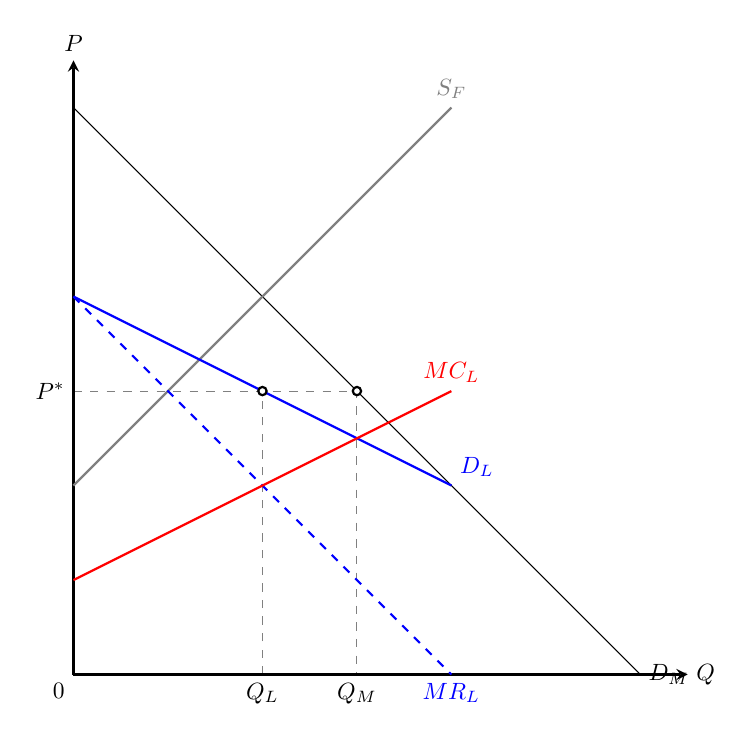
\begin{tikzpicture}[x=1.2cm, y=1.2cm, >=stealth, thick, every node/.style={scale=0.85}]
				% 1. 全局辅助虚线
				\draw[dashed, gray, thin] (0,3) -- (3,3) -- (3,0);
				\draw[dashed, gray, thin] (2,0) -- (2,3);
				
				% 2. 坐标轴与分离标签
				\draw[->] (0,0) -- (6.5,0) node[right] {$Q$};
				\draw[->] (0,0) -- (0,6.5) node[above] {$P$};
				\node[below left] at (0,0) {$0$};
				\node[left] at (0,3) {$P^*$};
				\node[below] at (2,0) {$Q_L$};
				\node[below] at (3,0) {$Q_M$};
				
				% 3. 严格定义域下的供需曲线群
				\draw[domain=0:6, color=black, thin] plot (\x, {6 - \x}) node[right] {$D_M$};
				\draw[domain=0:4, color=gray] plot (\x, {2 + \x}) node[above] {$S_F$};
				\draw[domain=0:4, color=blue] plot (\x, {4 - 0.5*\x}) node[above right] {$D_L$};
				\draw[domain=0:4, color=blue, dashed] plot (\x, {4 - \x}) node[below] {$MR_L$};
				\draw[domain=0:4, color=red] plot (\x, {1 + 0.5*\x}) node[above] {$MC_L$};
				
				% 4. 关键均衡点遮罩管理
				\filldraw[fill=white, draw=black] (2,3) circle (1.5pt);
				\filldraw[fill=white, draw=black] (3,3) circle (1.5pt);
			\end{tikzpicture}
		\end{center}
		
		\item \textbf{为什么欧佩克石油卡特尔成功地将价格抬高了许多，而西佩克铜卡特尔却做不到？什么条件是成功的卡特尔化所必需的？一个卡特尔必须克服什么组织上的问题？}
		
		\textbf{答：}
		欧佩克与西佩克在控价能力上的巨大差异，主要取决于市场供求弹性的根本不同。欧佩克成员国的核心石油产量占全球比重极高，且在短期内，全球对石油的总需求以及非欧佩克国家的潜在供给都极度缺乏弹性，这赋予了欧佩克强大的垄断势力。相反，铜的替代品众多（如铝的低成本替代），导致全球对铜的总需求富有弹性；同时，非西佩克成员国的铜矿短期供给弹性较大，极易通过扩产稀释控价效果，导致西佩克难以维持高价。
		
		成功的卡特尔化必须满足以下三个核心前提条件：一是行业潜在的垄断势力巨大，即该商品的总市场需求极缺乏弹性；二是卡特尔组织必须控制全球绝大部分的供给份额，且非卡特尔厂商的供给弹性极低；三是组织内部具备高效的协调与惩罚机制。
		
		在组织层面上，卡特尔必须克服的核心问题是如何在各成员国之间公平地分配产量限额与达成价格协议，以及如何建立透明的监督机制来有效遏制和惩罚成员国单方面超产偷跑的违约行为。
	\end{enumerate}
	\section{练习题}
	\begin{enumerate}[label=\textbf{\arabic*.}, leftmargin=*]
		\item \textbf{假设在一个垄断竞争行业中的所有厂商都被并入一个大企业。这个新企业会仍然生产那么多品牌吗？或者它会只生产一种单一品牌？请解释。}
		
		\textbf{答：}
		合并后的垄断企业既不会盲目保留原有的全部品牌，也不会彻底精简至单一品牌。
		
		新企业不会保留全部品牌，是因为垄断竞争市场原本存在的诸多细分品牌之间具有极高的替代性。保留过多的品牌不仅会带来高昂的重复固定资产运营成本，还会导致企业内部各品牌之间的恶性同室操戈，蚕食整体利润。
		
		然而，新企业同样不会只生产一种单一品牌。由于消费者面临异质化的偏好偏向，保留数个具有明显特征和价格梯度的核心品牌，是垄断者对市场进行消费者群体细分、实施间接价格歧视以榨取更多消费者剩余的有效手段。此外，保持适度的产品差异化能够有效刺激市场的总需求，从而实现比单一品牌更高的总体销售规模与垄断利润。
		
		\item \textbf{考虑下面的两家厂商。他们面临的需求曲线是 $P = 50 - 5Q$ 给出，其中 $Q = Q_1 + Q_2$。厂商的成本函数 $C_1(Q_1) = 20 + 10Q_1$ 和 $C_2(Q_2) = 10 + 12Q_2$。}
		
		\begin{enumerate}
			\item \textbf{假设两厂商都已进入了该行业。共同利润最大化的产量水平是多少？各厂商将生产多少？如果两厂商还都没有进入该行业，你的回答将如何改变？}
			\item \textbf{如果两厂商的行为非常不合作, 各厂商的均衡产量和利润是多少？利用古诺模型，画出两厂商的反应曲线，并表示出均衡。}
			\item \textbf{如果共谋是非法的但吞并却并不违法，厂商 1 会愿意出多少钱收购厂商 2？}
		\end{enumerate}
		
		\textbf{解：}
		(1) 由成本函数求导可知两工厂的边际成本分别为 $MC_1 = 10$ 和 $MC_2 = 12$。由于厂商 1 的边际成本在任何产量下均低于厂商 2，多厂垄断企业为了实现全行业共同利润最大化，应当将全部产量交由工厂 1 生产，即令 $Q_2 = 0$。
		
		此时整体大企业的利润函数及一阶导数条件为：
		\[
		\begin{aligned}
			\pi_T &= (50 - 5Q_1)Q_1 - 20 - 10Q_1 - 10 \\
			\frac{\mathrm{d}\pi_T}{\mathrm{d}Q_1} &= 40 - 10Q_1 = 0
		\end{aligned}
		\]
		解得整体最优决策为 $Q_1 = 4$，$Q_2 = 0$，出清价格 $P = 30$。此时各厂商利润分别为：
		\[
		\begin{aligned}
			\pi_1 &= 30 \times 4 - (20 + 10 \times 4) = 60 \\
			\pi_2 &= 30 \times 0 - (10 + 12 \times 0) = -10
		\end{aligned}
		\]
		此时行业的总利润为 $\pi_T = 60 - 10 = 50$ 美元。
		
		若两厂商均未进入行业，由于不需承担厂商 2 的 10 美元沉没固定成本，联合企业将彻底不建立工厂 2，行业总利润将提升为 $\pi_T = 60$ 美元（其中 $Q_1 = 4, Q_2 = 0$）。
		
		(2) 在此产量空间的古诺博弈中，两厂商的策略互动由其最优反应曲线展现，而非传统的价格需求曲线。需求曲线 $D$ 刻画的是价格与数量的总量关系，存在于 $P-Q$ 空间中；而本图所处的 $Q_1-Q_2$ 空间属于策略产出空间，其曲线 $R_1$ 与 $R_2$ 分别代表在给定竞争对手产量的前提下，各自最大化个体利润的纳什最优反应函数。
		\[
		\begin{aligned}
			R_1: \quad Q_1 &= 4 - 0.5Q_2 \\
			R_2: \quad Q_2 &= 3.8 - 0.5Q_1
		\end{aligned}
		\]
		
		通过联立上述反应函数，两条曲线的交点即为非合作博弈的古诺纳什均衡点 $E$。此时，双方均实现了给定对手产量下的个体最优决策，均衡产量分别为 $Q_1 = 2.8$，$Q_2 = 2.4$。
		
		\begin{center}
			\begin{tikzpicture}[x=1.3cm, y=1.3cm, >=stealth, thick, every node/.style={scale=0.85}]
				% 1. 全局辅助虚线 (最底层，精准锁定均衡点投影)
				\draw[dashed, gray, thin] (0,2.4) -- (2.8,2.4) -- (2.8,0);
				
				% 2. 坐标轴与物理分离标签 (彻底杜绝字体重叠)
				\draw[->] (0,0) -- (5.2,0) node[right] {$Q_1$};
				\draw[->] (0,0) -- (0,5.2) node[above] {$Q_2$};
				\node[below left] at (0,0) {$0$};
				\node[below] at (2.8,0) {$2.8$};
				\node[below] at (4,0) {$4$};
				\node[left] at (0,2.4) {$2.4$};
				\node[left] at (0,3.8) {$3.8$};
				
				% 3. 反应曲线实线 (对 R_1 的左侧定义域进行严格下限截断，防直冲云霄)
				\draw[domain=1.6:4, samples=50, color=blue] plot (\x, {8 - 2*\x});
				\node[blue, above right] at (1.6,4.8) {$R_1$};
				
				\draw[domain=0:5.0, samples=50, color=red] plot (\x, {3.8 - 0.5*\x}) node[right] {$R_2$};
				
				% 4. 均衡点与标号 (fill=white 遮罩管理，清除交叉线干扰)
				\filldraw[fill=white, draw=black] (2.8,2.4) circle (1.5pt) node[above right, fill=white, inner sep=1.5pt] {$E$};
			\end{tikzpicture}
		\end{center}
		
		(3) 厂商 1 愿意支付的最高收购对价，取决于吞并厂商 2 后所能实现的行业垄断总利润与原古诺非合作状态下自身利润的差额。
		
		由于两家厂商在此前均已进入该行业，厂商 2 的 10 美元固定成本已经沉没。厂商 1 收购厂商 2 后，作为理性的多工厂垄断者，会关停高成本的工厂 2（$Q_2 = 0$）并将生产集中于工厂 1（$Q_1 = 4$），此时新合并大企业的全行业总利润为 $\pi_T = 50$ 美元。
		
		因为兼并意味着厂商 1 必须统筹承担全行业的成本与收益，故其兼并后的最大净利润为 50 美元。已知兼并前厂商 1 的古诺个体利润为 19.2 美元，因此厂商 1 愿意支付的最高收购价格为：
		\[ W = \pi_T - \pi_1 = 50 - 19.2 = 30.8 \text{（美元）} \]
		\newpage
		
		\item \textbf{某垄断者能够以常数平均（和边际）成本 $AC = MC = 5$ 生产。该厂商面对的市场需求曲线是 $Q = 53 - P$。}
		
		\begin{enumerate}
			\item \textbf{计算这个垄断者的利润最大化价格和产量，并算出它的利润。}
			\item \textbf{假设第二个厂商加入该市场。$Q_1$ 为第一个厂商的产量，$Q_2$ 是第二个厂商的产量。市场需求现在由 $Q_1 + Q_2 = 53 - P$ 给出。设第二个厂商与第一个厂商有相同的成本，将各厂商的利润写成 $Q_1$ 和 $Q_2$ 的函数。}
			\item \textbf{假设（如在古诺模型中一样）各厂商在假定它的竞争者的产量固定时选择其利润最大化产量水平。求出各厂商的“反应曲线”。}
			\item \textbf{计算古诺均衡。求出市场价格和各厂商的利润是多少？}
			\item \textbf{设该行业中有 $N$ 家厂商，都有相同的常数边际成本 $MC = 5$。求出古诺均衡。各厂商将生产多少，市场价格为多少，以及各厂商将赚到多少利润？还有，证明当 $N$ 变大时，市场价格接近于完全竞争下的价格。}
		\end{enumerate}
		
		\textbf{解：}
		(1) 垄断厂商的反需求函数为 $P = 53 - Q$，其总收益函数为 $R = (53 - Q)Q$。由利润最大化的一阶条件：
		\[
		\begin{aligned}
			\frac{\mathrm{d}\pi}{\mathrm{d}Q} = \frac{\mathrm{d}R}{\mathrm{d}Q} - MC = 53 - 2Q - 5 = 0
		\end{aligned}
		\]
		解得利润最大化产量 $Q = 24$，代入需求方程得均衡价格 $P = 29$。此时垄断利润为：
		\[ \pi = (29 - 5) \times 24 = 576 \]
		
		(2) 引入双寡头竞争后，市场出清价格为 $P = 53 - Q_1 - Q_2$。两厂商的利润函数分别表示为：
		\[
		\begin{aligned}
			\pi_1 &= (53 - Q_1 - Q_2)Q_1 - 5Q_1 = 48Q_1 - Q_1^2 - Q_1Q_2 \\
			\pi_2 &= (53 - Q_1 - Q_2)Q_2 - 5Q_2 = 48Q_2 - Q_2^2 - Q_1Q_2
		\end{aligned}
		\]
		
		(3) 各厂商通过将对手产量视为常数来最大化自身利润。对利润函数求偏导并令其为 0：
		\[
		\begin{aligned}
			\frac{\partial\pi_1}{\partial Q_1} = 48 - 2Q_1 - Q_2 = 0 \implies R_1: \quad Q_1 = 24 - 0.5Q_2 \\
			\frac{\partial\pi_2}{\partial Q_2} = 48 - 2Q_2 - Q_1 = 0 \implies R_2: \quad Q_2 = 24 - 0.5Q_1
		\end{aligned}
		\]
		
		(4) 联立两厂商的反应曲线方程，解得古诺均衡产量为 $Q_1 = Q_2 = 16$。此时市场总产量为 32，均衡价格为 $P = 53 - 32 = 21$。各厂商的非合作均衡利润为：
		\[ \pi_1 = \pi_2 = (21 - 5) \times 16 = 256 \]
		
		(5) 当存在 $N$ 家代表性厂商时，市场价格方程扩展为 $P = 53 - \sum_{j=1}^N Q_j$。第 $i$ 家厂商的利润最大化条件为：
		\[
		\begin{aligned}
			\frac{\partial\pi_i}{\partial Q_i} = 53 - 2Q_i - \sum_{j \neq i} Q_j - 5 = 0
		\end{aligned}
		\]
		基于对称性假定，所有厂商的均衡产量均相等，即 $Q_i = Q^*$。上式可转化为：
		\[
		\begin{aligned}
			48 - 2Q^* - (N - 1)Q^* = 0 \implies Q^* = \frac{48}{N + 1}
		\end{aligned}
		\]
		由此可知，市场总产出为 $\frac{48N}{N + 1}$，代入反需求函数得到市场均衡价格为：
		\[ P = 53 - \frac{48N}{N + 1} = 5 + \frac{48}{N + 1} \]
		单家厂商的均衡利润为：
		\[ \pi_i = (P - MC)Q^* = \left(\frac{48}{N + 1}\right)^2 = \frac{2304}{(N + 1)^2} \]
		显然，当厂商数量趋于无穷时：
		\[
		\begin{aligned}
			\lim_{N \to \infty} P &= \lim_{N \to \infty} \left(5 + \frac{48}{N + 1}\right) = 5 \\
			\lim_{N \to \infty} \pi_i &= 0
		\end{aligned}
		\]
		此时市场价格恰好等于边际成本，超额利润完全消失，证明古诺市场结构在长期趋近于完全竞争均衡。
		
		\item \textbf{继续练习题 3。考虑两个具有相同常数平均和边际成本 $AC = MC = 5$ 的厂商，面临的市场需求曲线为 $Q_1 + Q_2 = 53 - P$。现在利用斯塔克博格模型来分析如果两厂商之一在另一厂商之前先作产量决策将会发生什么情况。}
		
		\begin{enumerate}
			\item \textbf{设厂商 1 是斯塔克博格领袖。找出反应曲线。}
			\item \textbf{各厂商将生产多少，以及利润为多少？}
		\end{enumerate}
		
		\textbf{解：}
		(1) 在序贯博弈中，后动厂商 2 面临既定的先前产量 $Q_1$，其最优化一阶条件导出的最优反应曲线与古诺模型一致：
		\[ Q_2 = 24 - 0.5Q_1 \]
		作为领导者的厂商 1 具有先行优势，不拥有传统的被动反应曲线，而是直接将厂商 2 的反应函数作为已知边界约束条件。
		
		(2) 厂商 1 将厂商 2 的策略代入自身的利润方程中进行独立求解：
		\[
		\begin{aligned}
			\max_{Q_1} \quad \pi_1 &= \left[53 - Q_1 - (24 - 0.5Q_1)\right]Q_1 - 5Q_1 = 24Q_1 - 0.5Q_1^2 \\
			\text{s.t.} \quad \frac{\mathrm{d}\pi_1}{\mathrm{d}Q_1} &= 24 - Q_1 = 0
		\end{aligned}
		\]
		解得领导者产量 $Q_1 = 24$。将其代入跟随者反应函数，得厂商 2 的产量 $Q_2 = 24 - 0.5 \times 24 = 12$。此时市场总产量为 36，出清价格降至 $P = 53 - 36 = 17$。两厂商的最终利润分别为：
		\[
		\begin{aligned}
			\pi_1 &= (17 - 5) \times 24 = 288 \\
			\pi_2 &= (17 - 5) \times 12 = 144
		\end{aligned}
		\]
		
		\newpage
		
		\item \textbf{两厂商生产相同的商品。它们同时选择的产出水平为 $Q_1$ 和 $Q_2$，面临的需求曲线为 $P = 30 - Q$，式中 $Q = Q_1 + Q_2$。直到最近，两家厂商的边际成本都为零。最近新颁布的环境法规使得厂商 2 的边际成本上升到 15 美元。厂商 1 的边际成本固定不变为零。判断正误：市场价格将因此上升到垄断水平。}
		
		\textbf{答：}
		该判断完全正确。
		
		在新的环境法规颁布后，厂商 1 的边际成本仍为 $MC_1 = 0$，其最优反应曲线可以通过最大化其个体利润导出：
		\[
		\begin{aligned}
			\max_{Q_1} \quad \pi_1 = (30 - Q_1 - Q_2)Q_1 \implies R_1: \quad Q_1 = 15 - 0.5Q_2
		\end{aligned}
		\]
		而厂商 2 的边际成本上升为 $MC_2 = 15$，其利润最大化的一阶条件发生相应改变：
		\[
		\begin{aligned}
			\max_{Q_2} \quad \pi_2 = (30 - Q_1 - Q_2)Q_2 - 15Q_2 \implies R_2: \quad Q_2 = 7.5 - 0.5Q_1
		\end{aligned}
		\]
		
		\begin{center}
			\begin{tikzpicture}[x=0.25cm, y=0.25cm, >=stealth, thick, every node/.style={scale=0.75}]
				% 1. 坐标轴与物理分离标签 (在微型尺寸下采用更精准的物理紧凑防重叠技术)
				\draw[->] (0,0) -- (22,0) node[right] {$Q_1$};
				\draw[->] (0,0) -- (0,22) node[above] {$Q_2$};
				\node[below left] at (0,0) {$0$};
				
				% 轴刻度标签物理位移微调，防止缩放后与轴线粘连
				\node[below=3pt] at (15,0) {$15$};
				\node[left=3pt] at (0,7.5) {$7.5$};
				
				% 2. 反应曲线实线 (严格保持定义域裁切，确保线条自然延伸而不外溢)
				% R1: Q2 = 30 - 2*Q1
				\draw[domain=5:15, samples=50, color=blue] plot (\x, {30 - 2*\x});
				\node[blue, right] at (5,20) {$R_1$};
				
				% R2: Q2 = 7.5 - 0.5*Q1
				\draw[domain=0:15, samples=50, color=red] plot (\x, {7.5 - 0.5*\x});
				\node[red, above right] at (0,7.5) {$R_2$};
				
				% 3. 边界纳什均衡点 (应用 fill=white 强力遮罩，彻底净化边界交叉视觉)
				\filldraw[fill=white, draw=black] (15,0) circle (2pt);
				\node[above right=4pt, fill=white, inner sep=1pt] at (15,0) {$E$};
			\end{tikzpicture}
		\end{center}
		
		如图所示，联立反应函数 $R_1$ 与 $R_2$ 进行求解，其交点恰好落在非负产量的几何边界上，即达成边界点纳什均衡 $E(15,0)$。此时，厂商 2 受到高额成本挤压，最优决策产量彻底萎缩至 $Q_2 = 0$ 并退出市场。全行业所有的供给完全由厂商 1 独家提供（$Q = Q_1 = 15$）。此时的市场价格为 $P = 30 - 15 = 15$。这一价格和产量配置恰好完全等同于厂商 1 在边际成本为 0 时单独面对市场所确立的完全垄断均衡，因此市场价格确实随之上升到了垄断水平。
		
		\newpage
		\item \textbf{设有两个某种商品的相同厂商，并且它们是市场上惟一的两个厂商。它们的成本由 $C_1 = 60Q_1$ 和 $C_2 = 60Q_2$ 给出，价格由需求函数给出：$P = 300 - Q$，其中 $Q = Q_1 + Q_2$。}
		
		\begin{enumerate}
			\item \textbf{求出古诺—纳什均衡。算出各厂商在该均衡中的利润。}
			\item \textbf{假设这两个厂商为了使联合利润最大化组成了一个卡特尔。它们将生产多少？算出各厂商的利润。}
			\item \textbf{设厂商 1 是该行业中惟一的厂商。市场产量和厂商 1 的利润与 (2) 中求出的有何不同？}
			\item \textbf{回到 (2) 中的双寡头，设厂商 1 遵守协定，但厂商 2 通过增产欺诈。厂商 2 将生产多少？各厂商的利润是多少？}
		\end{enumerate}
		
		\textbf{答：}
		\begin{enumerate}
			\item[(1)] 厂商 1 的利润最大化问题为 $\max_{Q_1} \pi_1 = (300 - Q_1 - Q_2)Q_1 - 60Q_1$。由一阶条件 $\frac{\partial\pi_1}{\partial Q_1} = 240 - 2Q_1 - Q_2 = 0$ 导出两厂商的反应曲线：
			\[
			\begin{aligned}
				R_1: \quad Q_1 &= 120 - 0.5Q_2 \\
				R_2: \quad Q_2 &= 120 - 0.5Q_1
			\end{aligned}
			\]
			联立解得古诺均衡产量 $Q_1 = Q_2 = 80$，市场总产量 $Q = 160$，出清价格 $P = 140$。各厂商的非合作利润为 $\pi_1 = \pi_2 = (140 - 60) \times 80 = 6400$。
			
			\item[(2)] 卡特尔旨在最大化联合利润：$\max_{Q} \pi_T = (300 - Q)Q - 60Q$。由一阶条件 $240 - 2Q = 0$ 解得行业垄断总产量 $Q = 120$，市场价格 $P = 180$。在对称成本下平分产量，即 $Q_1 = Q_2 = 60$，各厂商共谋利润为 $\pi_1 = \pi_2 = (180 - 60) \times 60 = 7200$。
			
			\item[(3)] 若厂商 1 为完全垄断者，其面临的利润最大化一阶条件与卡特尔完全一致。市场总产量仍为 $Q_1 = 120$，厂商 1 独享全部垄断利润 $\pi_1 = 14400$。由于边际成本为常数，多工厂共谋与单工厂垄断在总产量与总福利层面上没有差异。
			
			\item[(4)] 当厂商 1 遵守共谋产量 $Q_1 = 60$ 时，欺诈的厂商 2 将该产量视为既定约束，代入自身的反应曲线 $R_2$ 寻求个体利益最大化：
			\[ Q_2 = 120 - 0.5 \times 60 = 90 \]
			此时市场总产量扩充至 $Q = 150$，致使价格跌至 $P = 150$。各厂商利润结构转化为：
			\[
			\begin{aligned}
				\pi_1 &= (150 - 60) \times 60 = 5400 \\
				\pi_2 &= (150 - 60) \times 90 = 8100
			\end{aligned}
			\]
		\end{enumerate}
		
		该产量策略博弈如图所示。当双方达成共谋时，市场配置于 $M(60,60)$；若厂商 2 实施单方面欺诈，均衡点将横向右移至厂商 2 反应曲线上的 $C(60,90)$ 点；而双方理性的背叛最终会使市场跌回两条反应曲线的交点，即古诺纳什均衡点 $E_C(80,80)$。
		
		\begin{center}
			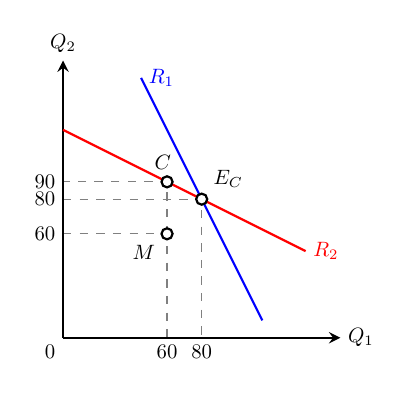
\begin{tikzpicture}[x=0.022cm, y=0.022cm, >=stealth, thick, every node/.style={scale=0.75}]
				% 1. 全局辅助虚线
				\draw[dashed, gray, thin] (0,80) -- (80,80) -- (80,0);
				\draw[dashed, gray, thin] (0,60) -- (60,60) -- (60,0);
				\draw[dashed, gray, thin] (60,60) -- (60,90) -- (0,90);
				
				% 2. 坐标轴与分离标签
				\draw[->] (0,0) -- (160,0) node[right] {$Q_1$};
				\draw[->] (0,0) -- (0,160) node[above] {$Q_2$};
				\node[below left] at (0,0) {$0$};
				\node[below] at (60,0) {$60$};
				\node[below] at (80,0) {$80$};
				\node[left] at (0,60) {$60$};
				\node[left] at (0,80) {$80$};
				\node[left] at (0,90) {$90$};
				
				% 3. 反应曲线 (严格裁切定义域防溢出)
				\draw[domain=45:115, samples=50, color=blue] plot (\x, {240 - 2*\x});
				\node[blue, right] at (45,150) {$R_1$};
				\draw[domain=0:140, samples=50, color=red] plot (\x, {120 - 0.5*\x}) node[right] {$R_2$};
				
				% 4. 关键博弈点标记
				\filldraw[fill=white, draw=black] (80,80) circle (2pt) node[above right, yshift=2pt,xshift=2pt] {$E_C$};
				\filldraw[fill=white, draw=black] (60,60) circle (2pt) node[below left,xshift=-2pt,yshift=-2pt] {$M$};
				\filldraw[fill=white, draw=black] (60,90) circle (2pt) node[above,yshift=2pt,xshift=-2pt] {$C$};
			\end{tikzpicture}
		\end{center}
		
		\item \textbf{假设两个竞争厂商 A 和 B 生产同质商品。两个厂商都有 $MC = 50$ 美元的边际成本。描述厂商在 (1) 古诺均衡，(2) 共谋均衡，(3) 伯特兰均衡中，产量和价格将发生什么变化。}
		
		\begin{enumerate}
			\item \textbf{因为厂商 A 必须增加工资，它的 $MC$ 上升到 80 美元。}
			\item \textbf{两个厂商的边际成本增加。}
			\item \textbf{需求曲线右移。}
		\end{enumerate}
		
		\textbf{答：}
		\begin{enumerate}
			\item[(1)] 当厂商 A 的边际成本上升至 80 美元，而 B 维持 50 美元时：在古诺均衡中，厂商 A 的最优反应曲线向内平移，导致其个体产量减少，而厂商 B 利用竞争空间扩大自身产量，最终行业总产量下降，出清价格上升。\\在共谋均衡中，多工厂垄断者为了最小化行业总成本，会选择彻底关停高成本的 A 工厂（产量归零），将生产完全配置于低成本的 B 工厂，此时全行业的总产量与价格由 B 独家垄断决定。\\在伯特兰均衡中，同质品价格战导致厂商 B 可以定价于略低于 A 边际成本的水平来独吞整个市场，从而将厂商 A 的销售份额压缩为零。
			
			\item[(2)] 当两厂商的边际成本均发生对称性上升时：在古诺均衡中，两者的反应曲线同时同步向内平移，导致两厂商的个体产量、行业总产量均出现萎缩，出清价格由于成本推动而被迫上升。\\在共谋均衡中，这等同于单厂商垄断边际成本线上移，企业会主动收缩总产量并调高市场零售价格。\\在伯特兰均衡中，由于恶性价格竞争直至边际成本的本质未变，均衡价格将直接被动推升至等于新的高边际成本水平，总市场销量下降。
			
			\item[(3)] 当市场总需求曲线发生向右外侧平移时：在古诺均衡中，伴随边际收益的扩张，两厂商的反应曲线相继向外平移，驱使两厂商的产量和市场出清价格同时上升。\\在共谋均衡中，垄断大企业面对右移的需求曲线与不变的边际成本，会同时扩大总产出并提升价格。\\在伯特兰均衡中，由于价格被死死锁定在边际成本线 $P = MC = 50$ 处，需求扩张将完全转化为行业销量的增加，市场均衡价格仍将保持恒定。
		\end{enumerate}
		
		\newpage
		\item \textbf{假设航空行业仅有两家厂商组成：美国航空公司和得克萨斯航空公司。让两厂商具有相同的成本函数 $C(q) = 40q$。设该行业的需求曲线为 $P = 100 - Q$，且各厂商都期望对方像古诺竞争者一样行为。}
		
		\begin{enumerate}
			\item \textbf{计算各厂商的古诺—纳什均衡。各厂商的利润是多少？}
			\item \textbf{如果得克萨斯航空具有常数边际成本和平均成本 25 美元，而美国航空具有常数边际成本和平均成本 40 美元，均衡产量为多少？}
			\item \textbf{假设两厂商原有成本函数为 $C(q) = 40q$，如果美国航空不会跟进，得克萨斯航空愿意投资多少资金以将它的边际成本从 40 美元降至 25 美元？如果不管美国航空怎么做，得克萨斯航空都有边际成本 25 美元，美国航空会愿意花费多少将它的边际成本降至 25 美元？}
		\end{enumerate}
		
		\textbf{解：}
		\begin{enumerate}
			\item[(1)] 由已知成本求导得 $MC_1 = MC_2 = 40$。美国航空的利润函数为 $\pi_1 = (100 - Q_1 - Q_2)Q_1 - 40Q_1$。由一阶条件 $$\frac{\partial\pi_1}{\partial Q_1} = 60 - 2Q_1 - Q_2 = 0$$
			得出两厂商的对称反应曲线：
			\[
			\begin{aligned}
				R_1: \quad Q_1 &= 30 - 0.5Q_2 \\
				R_2: \quad Q_2 &= 30 - 0.5Q_1
			\end{aligned}
			\]
			联立解得两航司的对称古诺产量为 $Q_1 = Q_2 = 20$，市场价格 $P = 60$。各厂商所获个体利润为 $\pi_1 = \pi_2 = (60 - 40) \times 20 = 400$ 美元。
			
			\item[(2)] 当得克萨斯航空（厂商 2）的成本下降至 $MC_2 = 25$ 时，美国航空（厂商 1）的反应曲线保持不变。得克萨斯航空的新决策一阶条件为 $100 - Q_1 - 2Q_2 - 25 = 0$，由此导出最新的非对称反应曲线群：
			\[
			\begin{aligned}
				R_1: \quad Q_1 &= 30 - 0.5Q_2 \\
				R_2': \quad Q_2 &= 37.5 - 0.5Q_1
			\end{aligned}
			\]
			联立解得新的非合作均衡产量为 $Q_1 = 15$，$Q_2 = 30$。此时全行业总产出 $Q = 45$，市场出清价格回落至 $P = 55$。
			
			\item[(3)] 在得克萨斯航空进行技术改造前，其所获古诺利润为 400 美元。若其单方面成功将边际成本压低至 25 美元而美航未更进，根据 (2) 的非对称均衡结果，市场价格变为 55 美元，得航新利润增加为 $\pi_2' = (55 - 25) \times 30 = 900$ 美元。因此，得克萨斯航空愿意为该项成本改善投入的最大资金上限为新旧利润的代数差额：
			\[ \Delta\pi_2 = 900 - 400 = 500 \text{（美元）} \]
			
			若得克萨斯航空的成本已固定在 25 美元，在美航尚未更进时，美航的初始利润受对手挤压降至 $\pi_1 = (55 - 40) \times 15 = 225$ 美元。此时，若美航同样花费资金将自身成本对等降至 25 美元，两厂商将重新返回对称古诺博弈，各自的反应曲线均优化为 $Q_i = 37.5 - 0.5Q_j$，解得对称总产出下 $Q_1 = Q_2 = 25$，均衡价格降至 $P = 50$ 美元。\\此时美航更进后的新利润为 $\pi_1' = (50 - 25) \times 25 = 625$ 美元。因此，在对手成本占优的被动情境下，美国航空为了进行战略防御愿意支付的最大投资额为：
			\[ \Delta\pi_1 = 625 - 225 = 400 \text{（美元）} \]
		\end{enumerate}
		
		该技术外生冲击带来的非对称古诺反应曲线平移轨迹如图所示。当得克萨斯航空（厂商 2）单方面降低成本时，其反应曲线由 $R_2$ 向上平行移动至 $R_2'$，市场均衡点顺势从原对称均衡点 $E_1(20,20)$ 转移至成本非对称的古诺均衡点 $E_2(15,30)$。
		
		\begin{center}
			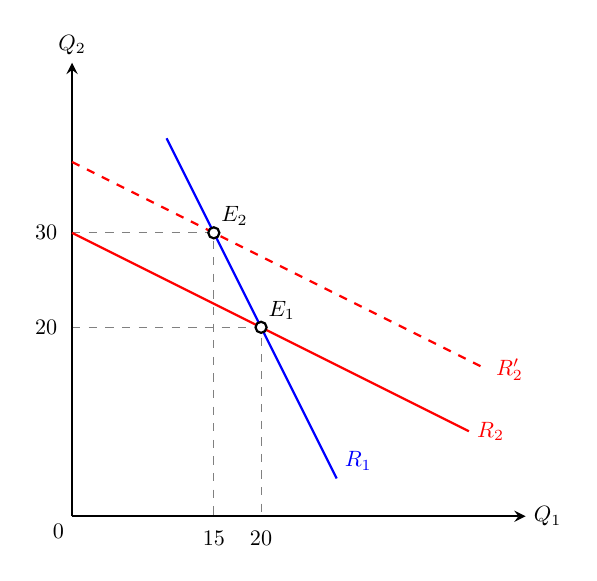
\begin{tikzpicture}[x=0.12cm, y=0.12cm, >=stealth, thick, every node/.style={scale=0.8}]
				% 1. 全局辅助虚线 (最底层，高精度对齐)
				\draw[dashed, gray, thin] (0,20) -- (20,20) -- (20,0);
				\draw[dashed, gray, thin] (0,30) -- (15,30) -- (15,0);
				
				% 2. 坐标轴与分离标签 (彻底解决高密度状态下的字体重叠)
				\draw[->] (0,0) -- (48,0) node[right] {$Q_1$};
				\draw[->] (0,0) -- (0,48) node[above] {$Q_2$};
				\node[below left] at (0,0) {$0$};
				\node[below=3pt] at (15,0) {$15$};
				\node[below=3pt] at (20,0) {$20$};
				\node[left=3pt] at (0,20) {$20$};
				\node[left=3pt] at (0,30) {$30$};
				
				% 3. 反应曲线实线 (精细化定义域裁剪，防止溢出视窗)
				% R1: Q2 = 60 - 2*Q1
				\draw[domain=10:28, samples=50, color=blue] plot (\x, {60 - 2*\x}) node[above right] {$R_1$};
				
				% R2: Q2 = 30 - 0.5*Q1
				\draw[domain=0:42, samples=50, color=red] plot (\x, {30 - 0.5*\x}) node[right] {$R_2$};
				
				% R2': Q2 = 37.5 - 0.5*Q1
				\draw[domain=0:44, samples=50, color=red, dashed] plot (\x, {37.5 - 0.5*\x}) node[right] {$R_2'$};
				
				% 4. 均衡点多图层标志 (运用 fill=white 擦除交叉辅助线的视觉噪音)
				\filldraw[fill=white, draw=black] (20,20) circle (2pt) node[above right=2pt, fill=white, inner sep=1pt] {$E_1$};
				\filldraw[fill=white, draw=black] (15,30) circle (2pt) node[above right=2pt, fill=white, inner sep=1pt] {$E_2$};
			\end{tikzpicture}
		\end{center}
		
		\item \textbf{对灯泡的需求为 $Q = 100 - P$，其中 $Q$ 以百万盒灯泡的销售计；$P$ 是每盒的价格。有两个灯泡生产商：永光和迪姆力。它们有相同的成本函数：$C_i = 10Q_i + \frac{1}{2}Q_i^2 \ (i = E, D)$，且 $Q = Q_E + Q_D$。}
		
		\begin{enumerate}
			\item \textbf{由于认识不到共谋的潜在可能，这两个厂商像短期完全竞争者一样行为。均衡的 $Q_E$、$Q_D$ 和 $P$ 的值各为多少？各厂商的利润是多少？}
			\item \textbf{两厂商的最高层经营者都被换掉了。双方新经理各自独立地认识到了灯泡行业的寡头垄断性质并采取古诺竞争策略。$Q_E$、$Q_D$ 和 $P$ 的均衡值又是多少？各厂商的利润是多少？}
			\item \textbf{假设永光的经理准确猜到迪姆力是采用古诺策略，所以永光采用斯塔克博格策略。$Q_E$、$Q_D$ 和 $P$ 的均衡值是多少？各厂商的利润是多少？}
			\item \textbf{如果两公司的经理共谋，$Q_E$、$Q_D$ 和 $P$ 的均衡值是多少？各厂商的利润是多少？}
		\end{enumerate}
		
		\textbf{答：}
		\begin{enumerate}
			\item[(1)] 完全竞争下，厂商依据价格等于边际成本原则提供产出。由成本函数求导得边际成本为 $MC_i = 10 + Q_i$。联立定价条件与市场需求方程：
			\[
			\begin{aligned}
				P &= 10 + Q_E \\
				P &= 10 + Q_D \\
				P &= 100 - Q_E - Q_D
			\end{aligned}
			\]
			解得完全竞争均衡产量为 $Q_E = 30$，$Q_D = 30$，出清价格为 $P = 40$。各厂商的个体利润为 $\pi_E = \pi_D = 450$。
			
			\item[(2)] 在古诺博弈中，两厂商通过选择自身产量来最大化利润。永光的利润最大化问题为：
			\[ \max_{Q_E} \quad \pi_E = (100 - Q_E - Q_D)Q_E - 10Q_E - 0.5Q_E^2 \]
			由一阶条件 $$\frac{\partial\pi_E}{\partial Q_E} = 90 - 3Q_E - Q_D = 0$$ 得出两厂商的最优反应曲线：
			\[ R_E: \quad Q_E = 30 - \frac{1}{3}Q_D \]
			\[ R_D: \quad Q_D = 30 - \frac{1}{3}Q_E \]
			联立解得古诺纳什均衡值：产量为 $Q_E = 22.5$，$Q_D = 22.5$，市场价格为 $P = 55$，各厂商的利润为 $\pi_E = \pi_D = 759.38$。
			
			\item[(3)] 在斯塔克博格模型中，先动领导者永光将跟随者迪姆力的反应曲线直接内生化到自身的利润函数中：
			\[ \max_{Q_E} \quad \pi_E = \left[100 - Q_E - \left(30 - \frac{1}{3}Q_E\right)\right]Q_E - 10Q_E - 0.5Q_E^2 = 60Q_E - \frac{7}{6}Q_E^2 \]
			由一阶最优化条件
			$$\frac{\mathrm{d}\pi_E}{\mathrm{d}Q_E} = 60 - \frac{7}{3}Q_E = 0$$ 
			解得：领导者产量为 $Q_E \approx 25.71$，跟随者产量为 $Q_D \approx 21.43$，最终市场出清价格为 $P \approx 52.86$。两厂商最终实现的非合作利润分别为 $\pi_E \approx 771.43$，$\pi_D \approx 688.78$。
			
			\item[(4)] 卡特尔共谋下，两厂商最大化行业总利润并等分产出。全行业总成本函数为：
			\[ TC = 2 \times \left[10\left(\frac{Q}{2}\right) + 0.5\left(\frac{Q}{2}\right)^2\right] = 10Q + 0.25Q^2 \]
			联合利润最大化的一阶条件为：
			\[ \frac{\mathrm{d}\pi_T}{\mathrm{d}Q} = 100 - 2Q - 10 - 0.5Q = 0 \]
			解得全行业垄断总产量为 $Q = 36$，两厂商平分产量为 $Q_E = Q_D = 18$，市场均衡价格上升至 $P = 64$。此时各厂商均实现最大化卡特尔共谋利润 $\pi_E = \pi_D = 810$。
		\end{enumerate}
		
		\begin{center}
			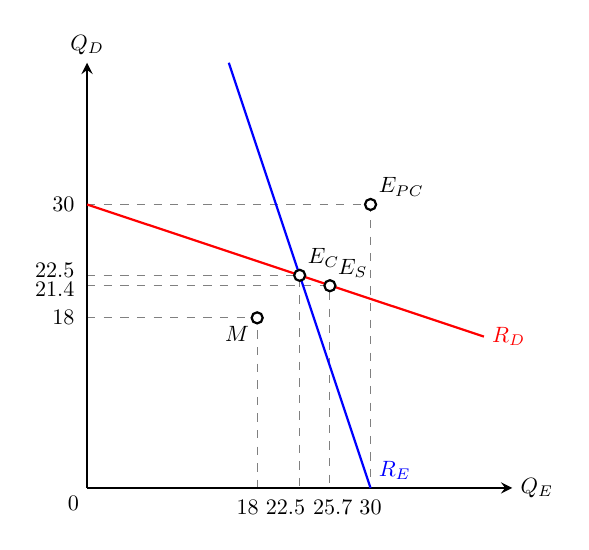
\begin{tikzpicture}[x=0.12cm, y=0.12cm, >=stealth, thick, every node/.style={scale=0.8}]
				\draw[dashed, gray, thin] (0,30) -- (30,30) -- (30,0);
				\draw[dashed, gray, thin] (0,22.5) -- (22.5,22.5) -- (22.5,0);
				\draw[dashed, gray, thin] (0,21.4) -- (25.7,21.4) -- (25.7,0);
				\draw[dashed, gray, thin] (0,18) -- (18,18) -- (18,0);
				
				\draw[->] (0,0) -- (45,0) node[right] {$Q_E$};
				\draw[->] (0,0) -- (0,45) node[above] {$Q_D$};
				\node[below left] at (0,0) {$0$};
				\node[below=2pt] at (17,0) {$18$};
				\node[below=2pt] at (21,0) {$22.5$};
				\node[below=2pt] at (26,0) {$25.7$};
				\node[below=2pt] at (30,0) {$30$};
				\node[left=2pt] at (0,18) {$18$};
				\node[left=2pt] at (0,21) {$21.4$};
				\node[left=2pt] at (0,23) {$22.5$};
				\node[left=2pt] at (0,30) {$30$};
				
				\draw[domain=15:30, samples=50, color=blue] plot (\x, {90 - 3*\x}) node[above right] {$R_E$};
				\draw[domain=0:42, samples=50, color=red] plot (\x, {30 - 0.333*\x}) node[right] {$R_D$};
				
				\filldraw[fill=white, draw=black] (30,30) circle (2pt) node[above right] {$E_{PC}$};
				\filldraw[fill=white, draw=black] (22.5,22.5) circle (2pt) node[above right] {$E_C$};
				\filldraw[fill=white, draw=black] (25.7,21.4) circle (2pt) node[above right] {$E_S$};
				\filldraw[fill=white, draw=black] (18,18) circle (2pt) node[below left] {$M$};
			\end{tikzpicture}
		\end{center}
		\newpage
		\item \textbf{两厂商生产豪华型羊皮自动椅套：Western Where（WW）和 B.B.B. Sheep（BBBS）。每家厂商的成本函数为：$C(q)=30q+1.5q^2$。市场价格由反需求方程给出：$P=300-3Q$，式中总产出 $Q=q_w + q_b$。}
		
		\begin{enumerate}
			\item \textbf{如果每家厂商在给定对手产出的情况下追求利润极大化，每家厂商将选择的均衡产量、总产出和市场价格为多少？每家厂商各自的利润又为多少？}
			\item \textbf{如果两家厂商共谋，利润最大化时的产出、市场价格以及各厂商各自的产出和利润为多少？}
			\item \textbf{每家厂商必须独自决定是生产古诺数量还是生产卡特尔数量。重新构建利润支付矩阵，并说明每家厂商会采取怎样的产出策略。}
			\item \textbf{假设 WW 能在 BBBS 之前确定产出水平。在此情况下，各厂商将选择怎样的产量？市场价格和利润为多少？先发优势对 WW 有利吗？}
		\end{enumerate}
		
		\textbf{解：}
		\begin{enumerate}
			\item[(1)] 非合作产量竞争下，由个体利润极大化的一阶导数条件 $270 - 9q_w - 3q_b = 0$ 导出两厂商的反应曲线：
			\[ R_w: \quad q_w = 30 - \frac{1}{3}q_b \]
			\[ R_b: \quad q_b = 30 - \frac{1}{3}q_w \]
			联立解得两厂商的古诺纳什均衡产量为 $q_w = q_b = 22.5$，行业总产出为 $Q = 45$，市场出清价格为 $P = 165$。各厂商获得的非合作利润为 $\pi_w = \pi_b = 2278.13$。
			
			\item[(2)] 当两厂商达成卡特尔共谋时，旨在最大化联合垄断利润：
			\[ \max_{Q} \quad \pi_T = (300 - 3Q)Q - 2 \times \left[30\left(\frac{Q}{2}\right) + 1.5\left(\frac{Q}{2}\right)^2\right] = 270Q - 3.75Q^2 \]
			由一阶优化条件 $$\frac{\mathrm{d}\pi_T}{\mathrm{d}Q} = 270 - 7.5Q = 0$$ 解得全行业最优总产量为 $Q = 36$，两厂商平分产出为 $q_w = q_b = 18$。此时市场零售价格上升至 $P = 192本地$，各厂商共谋利润优化为 $\pi_w = \pi_b = 2430$。
			
			\item[(3)] 若一方单方面扩产至古诺产量而另一方坚守协议，市场总产量为 $Q = 40.5$，价格为 $P = 178.5$。此时扩产方利润为 $2581.88$，守约方利润为 $2187$。博弈的支付矩阵如下：
			
			\begin{center}
				\renewcommand{\arraystretch}{1.4}
				\setlength{\tabcolsep}{6pt}
				\begin{tabular}{cc|c|c|}
					& \multicolumn{1}{c}{} & \multicolumn{2}{c}{BBBS} \\
					& \multicolumn{1}{c}{} & \multicolumn{1}{c}{古诺 ($22.5$)} & \multicolumn{1}{c}{卡特尔 ($18$)} \\
					\cline{3-4}
					& 古诺 ($22.5$) & $(2278.13, 2278.13)$ & $(2581.88, 2187.00)$ \\
					\cline{3-4}
					WW & 卡特尔 ($18$) & $(2187.00, 2581.88)$ & $(2430.00, 2430.00)$ \\
					\cline{3-4}
				\end{tabular}
			\end{center}
			
			矩阵表明，无论对手如何决策，选择古诺产量均是个体厂商的占优策略。这构成了囚徒困境，两厂商最终会由于非合作策略趋向于生产古诺数量，收敛于唯一的纳什均衡 $(2278.13, 2278.13)$。
			
			\item[(4)] 在斯塔克博格序贯博弈中，领导者 WW 将跟随者 BBBS 的反应函数直接代入自身的利润函数中：
			\[ \max_{q_w} \quad \pi_w = \left[300 - 3q_w - 3\left(30 - \frac{1}{3}q_w\right)\right]q_w - (30q_w + 1.5q_w^2) = 180q_w - 3.5q_w^2 \]
			由一阶条件 $180 - 7q_w = 0$，解得领导者最优产量为 $q_w \approx 25.71$，跟随者被动产量缩减为 $q_b \approx 21.43$。此时市场总产出为 $Q \approx 47.14$，出清价格为 $P \approx 158.57$，两厂商最终利润分别为 $\pi_w \approx 2314.29$ 和 $\pi_b \approx 2066.33$。
			
			这一结果表明先发优势对 WW 有利。由于抢先决定产量具有不可逆的承诺效应，WW 获得了比古诺均衡更高的个体利润。
			\end{enumerate}
		\item \textbf{两厂商通过选择价格竞争，它们的需求曲线是：$Q_1 = 20 - P_1 + P_2$ 和 $Q_2 = 20 + P_1 - P_2$。其中，$P_1$ 和 $P_2$ 分别是两厂商所定的价格；$Q_1$ 和 $Q_2$ 则是相应的需求。边际成本为零。}
		
		\begin{enumerate}
			\item \textbf{设两厂商同时决定它们的价格，求出相应的纳什均衡。各厂商会定什么价格，它们将销出多少，利润为多少？}
			\item \textbf{设厂商 1 先定价格，然后厂商 2 定价。各厂商将定价多少？能销出多少？利润为多少？}
			\item \textbf{设你是两厂商之一，且你们有三种博弈的方法：(1) 两厂商同时定价；(2) 你先定价；(3) 你的竞争者先定价。如果能从中选择，你喜欢哪种？解释原因。}
		\end{enumerate}
		
		\textbf{答：}
		\begin{enumerate}
			\item[(1)] 边际成本为零时，利润等于总收益。两厂商同时决策时的目标函数为：
			\[
			\begin{aligned}
				\max_{P_1} \quad \pi_1 = 20P_1 - P_1^2 + P_1P_2 \\
				\max_{P_2} \quad \pi_2 = 20P_2 - P_2^2 + P_1P_2
			\end{aligned}
			\]
			由一阶最优化条件：
			\[ 20 - 2P_1 + P_2 = 0 \]
			\[ 20 + P_1 - 2P_2 = 0 \]
			联立解得价格竞争的对称纳什均衡值为 $P_1 = P_2 = 20$。此时各厂商销量为 $Q_1 = Q_2 = 20$，个体利润为 $\pi_1 = \pi_2 = 400$。
			
			\item[(2)] 厂商 1 先定价时，后动厂商 2 依据自身的最优反应曲线决策：
			\[ P_2 = 10 + 0.5P_1 \]
			厂商 1 将该约束内生化到自身的利润函数中：
			\[ \max_{P_1} \quad \pi_1 = P_1\left[20 - P_1 + (10 + 0.5P_1)\right] = 30P_1 - 0.5P_1^2 \]
			由一阶条件 $30 - P_1 = 0$ 解得领导者价格 $P_1 = 30$。代入反应曲线得跟随者价格 $P_2 = 25$。此时两厂商销量分别为 $Q_1 = 15$ 和 $Q_2 = 25$，最终利润分别为 $\pi_1 = 450$ 和 $\pi_2 = 625$。
			
			\item[(3)] 理性厂商首选策略(3)，次选策略(2)，最末选策略(1)。在产品有差异的价格竞争中，两厂商的价格互为战略补充品，最优反应曲线斜率为正。序贯博弈中先动者提价会引导后动者协同提价，使双方价格均高于同时定价基准，因而两种序贯博弈利润均优于同时定价。然而，后动厂商可以利用后发优势实施价格拦截，从而截留更大的市场份额，获得比先动者更高的个体利润（$625 > 450$）。
		\end{enumerate}
		\newpage
		\item \textbf{主导厂商模型可以帮助理解某些卡特尔的行为。将这种模型应用于欧佩克石油卡特尔。世界需求 $W$ 和非卡特尔供给 $S$ 方程为：$W = 160P^{-1/2}$，$S = \frac{10}{3}P^{1/2}$。欧佩克的净需求为 $D = W - S$，且设欧佩克的生产成本为零。}
		
		\begin{enumerate}
			\item \textbf{画出世界需求曲线 $W$，非欧佩克供给曲线 $S$，欧佩克的需求曲线 $D$，以及欧佩克的边际收益曲线，指出欧佩克的最优价格与产量配置，并分析非欧佩克储量枯竭时的曲线平移特征。}
			\item \textbf{计算欧佩克的最优（利润最大化）价格。}
			\item \textbf{假设石油消费国想要联合起来并形成一个“买方的卡特尔”以得到买方垄断势力。关于这会对价格造成的冲击，可以确定的是什么？不能确定的是什么？}
		\end{enumerate}
		
		\textbf{答：}
		\begin{enumerate}
			\item[(1)] 主导厂商模型均衡如图所示。主导厂商欧佩克面对的是世界总需求 $W$ 减去非卡特尔供给 $S$ 后沉淀出的残差净需求曲线 $D$。依据 $MR = MC = 0$ 确立最优控价 $P^*$，非卡特尔厂商在此价格下供给 $Q_S^*$，全市场总产出为 $Q_W^*$。
			
			若非欧佩克石油储量枯竭导致其供给成本增大，其供给曲线 $S$ 将向左上方平移。在相同的价格水平下，外部竞争性供给的减少会迫使欧佩克面临的残差需求曲线 $D$ 连同其边际收益曲线 $MR$ 整体向右上方平移，最终推高全行业均衡油价。
			
			\begin{center}
				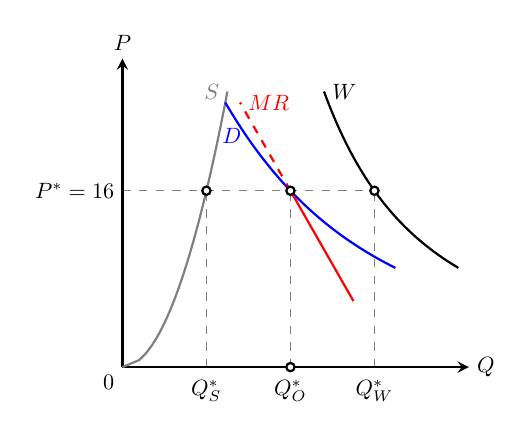
\begin{tikzpicture}[x=0.08cm, y=0.14cm, >=stealth, thick, every node/.style={scale=0.8}]
					% 1. 全局辅助虚线 (最底层投影)
					\draw[dashed, gray, thin] (0,16) -- (40,16);
					\draw[dashed, gray, thin] (13.33,0) -- (13.33,16);
					\draw[dashed, gray, thin] (26.67,0) -- (26.67,16);
					\draw[dashed, gray, thin] (40,0) -- (40,16);
					
					% 2. 坐标轴与分离标签 (轴长55，最大数据53.33，完美防溢出)
					\draw[->] (0,0) -- (55,0) node[right] {$Q$};
					\draw[->] (0,0) -- (0,28) node[above] {$P$};
					\node[below left] at (0,0) {$0$};
					\node[left] at (0,16) {$P^*=16$};
					\node[below=2pt] at (13.33,0) {$Q_S^*$};
					\node[below=2pt] at (26.67,0) {$Q_O^*$};
					\node[below=2pt] at (40,0) {$Q_W^*$};
					
					% 3. 严格定义域裁剪，规避无限延伸
					\draw[domain=9:25, samples=60, color=black] plot ({160/sqrt(\x)}, \x) node[right] {$W$};
					\draw[domain=0:25, samples=40, color=gray] plot ({(10/3)*sqrt(\x)}, \x) node[left] {$S$};
					\draw[domain=9:24, samples=50, color=blue] plot ({160/sqrt(\x) - (10/3)*sqrt(\x)}, \x) node[below,yshift=-8pt,xshift=3pt] {$D$};
					
					% MR 曲线精确截断
					\draw[domain=6:16, samples=20, color=red] plot ({42.67 - 1*(\x)}, \x);
					\draw[domain=16:24, samples=20, color=red, dashed] plot ({42.67 - 1*(\x)}, \x) node[right] {$MR$};
					
					% 4. 关键交点标号 (fill=white 擦除交叉线干扰)
					\filldraw[fill=white, draw=black] (13.33,16) circle (1.5pt);
					\filldraw[fill=white, draw=black] (26.67,16) circle (1.5pt);
					\filldraw[fill=white, draw=black] (40,16) circle (1.5pt);
					\filldraw[fill=white, draw=black] (26.67,0) circle (1.5pt);
				\end{tikzpicture}
			\end{center}
			
			\item[(2)] 欧佩克面临的残差需求曲线方程为 $Q = 160P^{-0.5} - \frac{10}{3}P^{0.5}$。由于边际成本为零，最大化利润即等价于最大化总收益：
			\[ \max_{P} \quad \pi = P \cdot Q = 160P^{0.5} - \frac{10}{3}P^{1.5} \]
			由利润极大化一阶条件：
			\[ \frac{\mathrm{d}\pi}{\mathrm{d}P} = 80P^{-1/2} - 5P^{1/2} = 0 \]
			方程两边同乘以 $P^{1/2}$ 化简得 $5P = 80$，解得欧佩克最优利润最大化价格为 $P = 16$。
			
			\item[(3)] 石油消费国组建买方卡特尔将使原市场演变为双边垄断结构。可以确定的是，买方势力的介入会产生压低油价的向下冲击。
			
			无法确定的是最终的均衡价格与贸易数量。双边垄断的价格在纯理论推导上具有不确定性，其最终结果取决于两个卡特尔集团之间的博弈与谈判力量对比。鉴于石油作为现代工业刚需、其短期需求极缺乏弹性的特征，买方潜在的对抗筹码有限，因而其对价格的实质性冲击将比较温和。
		\end{enumerate}
		\newpage
		\item \textbf{假设网球鞋市场有一个主导厂商和五个边缘厂商。市场需求为 $Q = 400 - 2P$。主导厂商有 $20$ 的不变的边际成本。每个边缘厂商有 $MC = 20 + 5q$ 的边际成本。}
		
		\begin{enumerate}
			\item \textbf{证明五家边缘厂商的总供给曲线为 $Q_f = P - 20$。}
			\item \textbf{求主导厂商的需求曲线。}
			\item \textbf{求利润最大化时的生产数量和主导厂商索取的价格，并求此时每个边缘厂商的生产数量和价格。}
			\item \textbf{假设有 10 个边缘厂商而不是 5 个，你的结果会有什么变化？}
			\item \textbf{假设仍为 5 个边缘厂商，但每个都设法将边际成本减少为 $MC = 20 + 2q$。你的结果会有什么变化？}
		\end{enumerate}
		
		\textbf{答：}
		\begin{enumerate}
			\item[(1)] 边缘厂商为价格接受者，按价格等于边际成本原则提供产品：
			\[ P = 20 + 5q \implies q = 0.2P - 4 \]
			因 5 家边缘厂商完全对称，水平加总得到总供给曲线：
			\[ Q_f = 5(0.2P - 4) = P - 20 \]
			
			\item[(2)] 主导厂商面临的市场残差需求曲线为市场总需求与边缘厂商总供给之差：
			\[ Q_d = (400 - 2P) - (P - 20) = 420 - 3P \]
			
			\item[(3)] 主导厂商通过令边际收益等于边际成本来最大化自身利润。反残差需求曲线为：
			\[ P = 140 - \frac{1}{3}Q_d \]
			由此导出主导厂商的边际收益函数：
			\[ MR_d = 140 - \frac{2}{3}Q_d \]
			由利润最大化条件 $MR_d = MC_d$：
			\[ 140 - \frac{2}{3}Q_d = 20 \]
			解得主导厂商的最优产量为 $Q_d = 180$，出清价格为 $P = 80$。边缘厂商索取相同价格，其总产量为 $Q_f = 80 - 20 = 60$，每家边缘厂商的产量为 $q = 12$。
		\end{enumerate}
		
		\newpage
		主导厂商模型的几何均衡状态如图所示。主导厂商面对的是市场总需求 $D_M$ 减去边缘供给 $S_f$ 后沉淀出的残差需求曲线 $D_d$。依据 $MR_d = MC_d$ 确立最优价格 $P^*$，边缘厂商在此价格下供给 $Q_f^*$，主导厂商供给 $Q_d^*$，市场总产出为 $Q_T^*$。
		
		\begin{center}
			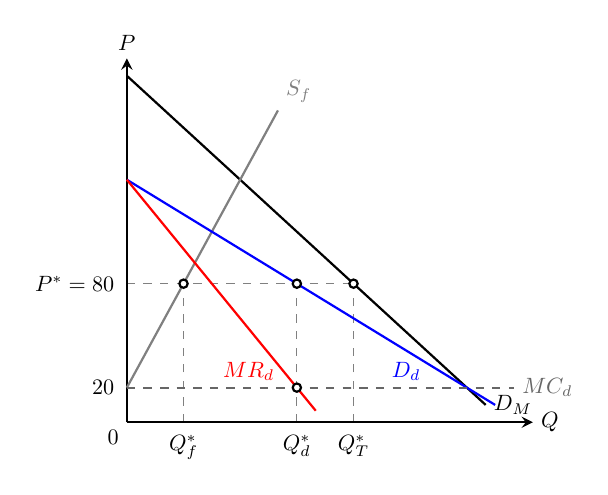
\begin{tikzpicture}[x=0.012cm, y=0.022cm, >=stealth, thick, every node/.style={scale=0.8}]
				% 1. 全局辅助虚线 (最底层投影)
				\draw[dashed, gray, thin] (0,80) -- (240,80);
				\draw[dashed, gray, thin] (180,0) -- (180,80);
				\draw[dashed, gray, thin] (60,0) -- (60,80);
				\draw[dashed, gray, thin] (240,0) -- (240,80);
				
				% 2. 坐标轴与分离标签
				\draw[->] (0,0) -- (430,0) node[right] {$Q$};
				\draw[->] (0,0) -- (0,210) node[above] {$P$};
				\node[below left] at (0,0) {$0$};
				\node[left=2pt] at (0,20) {$20$};
				\node[left=2pt] at (0,80) {$P^*=80$};
				\node[below=2pt] at (60,0) {$Q_f^*$};
				\node[below=2pt] at (180,0) {$Q_d^*$};
				\node[below=2pt] at (240,0) {$Q_T^*$};
				
				% 3. 严格定义域裁剪
				\draw[domain=0:380, samples=20, color=black] plot (\x, {200 - 0.5*\x}) node[right] {$D_M$};
				\draw[domain=0:160, samples=20, color=gray] plot (\x, {20 + \x}) node[above right] {$S_f$};
				\draw[domain=0:390, samples=20, color=blue] plot (\x, {140 - 0.3333*\x}) node[left,xshift=-30pt,yshift=15pt] {$D_d$};
				\draw[domain=0:200, samples=20, color=red] plot (\x, {140 - 0.6667*\x}) node[above left,xshift=-15pt,yshift=10pt] {$MR_d$};
				\draw[domain=0:410, samples=20, color=black!60, dashed] plot (\x, 20) node[right] {$MC_d$};
				
				% 4. 关键交点标号 (fill=white 擦除交叉线干扰)
				\filldraw[fill=white, draw=black] (180,20) circle (1.5pt);
				\filldraw[fill=white, draw=black] (60,80) circle (1.5pt);
				\filldraw[fill=white, draw=black] (180,80) circle (1.5pt);
				\filldraw[fill=white, draw=black] (240,80) circle (1.5pt);
			\end{tikzpicture}
		\end{center}
		
		\begin{enumerate}
			\item[]
			\item[(4)] 若有 10 家边缘厂商，则边缘总供给曲线转化为 $Q_f = 2P - 40$。主导厂商面临的新残差需求曲线为：
			\[ Q_d = (400 - 2P) - (2P - 40) = 440 - 4 P \]
			由反需求函数 $P = 110 - 0.25Q_d$ 导出边际收益 $MR_d = 110 - 0.5Q_d$。由 $MR_d = MC_d$ 条件：
			\[ 110 - 0.5Q_d = 20 \]
			解得主导厂商的产量仍为 $Q_d = 180$，但市场出清价格降至 $P = 65$。此时边缘厂商总供给增加为 $Q_f = 90$，单家边缘厂商供给变为 $q = 9$。主导厂商的市场份额由原来的 $75\%$ 稀释至 $66.7\%$。
			
			\item[(5)] 当单个边缘厂商成本下降时，其个体供给变为 $q = 0.5P - 10$，5 家边缘总供给拓展为 $Q_f = 2.5P - 50$。此时主导厂商面临的新残差需求曲线为：
			\[ Q_d = (400 - 2P) - (2.5P - 50) = 450 - 4.5P \]
			由反需求函数 $P = 100 - \frac{2}{9}Q_d$ 导出边际收益 $MR_d = 100 - \frac{4}{9}Q_d$。由 $MR_d = MC_d$ 条件：
			\[ 100 - \frac{4}{9}Q_d = 20 \]
			解得主导厂商产量依旧维持在 $Q_d = 180$，市场价格进一步跌至 $P = 60$。此时边缘厂商总供给增加为 $Q_f = 100$，单家边缘厂商供给提升为 $q = 20$。主导厂商的市场份额降至 $64.3\%$。
		\end{enumerate}
		\newpage
		\item \textbf{一个生产柠檬的卡特尔由四个果园组成。它们的总成本曲线为：}
		\[
		\begin{aligned}
			TC_1 &= 20 + 5Q_1^2 \\
			TC_2 &= 25 + 3Q_2^2 \\
			TC_3 &= 15 + 4Q_3^2 \\
			TC_4 &= 20 + 6Q_4^2
		\end{aligned}
		\]
		
		\begin{enumerate}
			\item \textbf{用表列出产量水平在每月 1 箱～5 箱之间时各果园的总成本、平均成本和边际成本。}
			\item \textbf{如果该卡特尔决定每月采运 10 箱并将价格定在每箱 25 美元，产量在果园之间应怎样分配？}
			\item \textbf{在这个采运量水平，哪个果园进行价格欺诈的冲动最大？是否哪个果园都没有进行价格欺诈的冲动吗？}
		\end{enumerate}
		
		\textbf{答：}
		\begin{enumerate}
			\item[(1)] 各果园在离散产量水平下的总成本 $TC$ 依据成本方程求得；平均成本由 $AC = TC / Q$ 计算；边际成本 $MC$ 为产量每增加 1 箱时总成本的离散增量（$\Delta TC$）。各果园成本结构重构如下：
			
			\begin{center}
				\renewcommand{\arraystretch}{1.2}
				\setlength{\tabcolsep}{5pt}
				\begin{tabular}{ccccccc}
					\hline
					& \multicolumn{3}{c}{果园 1} & \multicolumn{3}{c}{果园 2} \\
					\cline{2-4} \cline{5-7}
					产量 $Q$ & $TC$ & $AC$ & $MC$ & $TC$ & $AC$ & $MC$ \\
					\hline
					0 & 20 & ---  & --- & 25 & ---  & --- \\
					1 & 25 & 25.0 & 5   & 28 & 28.0 & 3   \\
					2 & 40 & 20.0 & 15  & 37 & 18.5 & 9   \\
					3 & 65 & 21.7 & 25  & 52 & 17.3 & 15  \\
					4 & 100& 25.0 & 35  & 73 & 18.3 & 21  \\
					5 & 145& 29.0 & 45  & 100& 20.0 & 27  \\
					\hline
				\end{tabular}
			\end{center}
			
			\begin{center}
				\renewcommand{\arraystretch}{1.2}
				\setlength{\tabcolsep}{5pt}
				\begin{tabular}{ccccccc}
					\hline
					& \multicolumn{3}{c}{果园 3} & \multicolumn{3}{c}{果园 4} \\
					\cline{2-4} \cline{5-7}
					产量 $Q$ & $TC$ & $AC$ & $MC$ & $TC$ & $AC$ & $MC$ \\
					\hline
					0 & 15 & ---  & --- & 20 & ---  & --- \\
					1 & 19 & 19.0 & 4   & 26 & 26.0 & 6   \\
					2 & 31 & 15.5 & 12  & 44 & 22.0 & 18  \\
					3 & 51 & 17.0 & 20  & 74 & 24.7 & 30  \\
					4 & 79 & 19.8 & 28  & 116& 29.0 & 42  \\
					5 & 115& 23.0 & 36  & 170& 34.0 & 54  \\
					\hline
				\end{tabular}
			\end{center}
			\newpage
			\item[(2)] 为了实现全行业联合成本最小化，产量的逐箱指派应遵循边际成本递增的最底层递补原则。逐箱最优分配路径如下：
			
			\begin{center}
				\renewcommand{\arraystretch}{1.1}
				\setlength{\tabcolsep}{12pt}
				\begin{tabular}{ccccccccccc}
					\hline
					箱数 & 1 & 2 & 3 & 4 & 5 & 6 & 7 & 8 & 9 & 10 \\
					\hline
					果园 & 2 & 3 & 1 & 4 & 2 & 3 & 1 & 2 & 4 & 3 \\
					\hline
				\end{tabular}
			\end{center}
			
			汇总分配结果，最终的配额配置为：果园 1 生产 $2$ 箱，果园 2 生产 $3$ 箱，果园 3 生产 $3$ 箱，果园 4 生产 $2$ 箱。
			
			\item[(3)] 果园 2 进行价格欺诈以单方面超产的冲动最大。在当前分配份额下，果园 2 生产第 4 箱柠檬的边际成本仅为 $21$，依然低于 $25$ 的卡特尔协议价，超产具有正的边际利润。
			
			相比之下，其他果园均缺乏违约欺诈的冲动。若果园 3 和果园 4 生产超出配额的下一箱，其边际成本（分别为 $28$ 和 $30$）将超过卡特尔售价，从而引发实质性亏损。果园 1 超产的下一箱边际成本恰好等于市场协议价（$25$），其超产的经济学边际激励同样为零。
		\end{enumerate}
	\end{enumerate}
	
	% =======================================================
	%                 第 13 章：博弈论与竞争策略
	% =======================================================
	\chapter{博弈论与竞争策略}
	
	\section{复习题}
	\begin{enumerate}[label=\textbf{\arabic*.}, leftmargin=*]
		\item \textbf{合作博弈和非合作博弈之间的区别是什么？各举出一个例子。}
		
		\textbf{答：}
		合作博弈与非合作博弈的核心区别在于参与人之间能否达成具有法律或外部强制约束力的协议。\\在合作博弈中，参与人能够通过谈判制定约束双方共同策略的合同，从而追求团队理性与联合利润最大化；而在非合作博弈中，由于制度缺失、履约成本过高或信息不对称，参与人无法达成或强制执行此类有约束力的合同，博弈各方只能基于个人理性独立进行策略选择。例如，两家企业联合开发一项新技术，若能签订一份具有法律效力且能有效分配联合投资利润的合同，则属于合作博弈；相反，若两家竞争企业在无法勾结的环境下，相互预测对方的行为并独立制定价格或广告策略以争夺市场份额，则属于典型的非合作博弈。
		
		\item \textbf{什么是占优策略？为什么一个占优策略均衡是稳定的？}
		
		\textbf{答：}
		占优策略是指无论对手采取何种策略，参与人所能选择的唯一绝对最优策略。设参与人 $i$ 的策略空间为 $S_i$，对手的策略组合为 $s_{-i}$，若策略 $s_i^* \in S_i$ 满足：
		\[
		\begin{aligned}
			u_i(s_i^*, s_{-i}) \ge u_i(s_i, s_{-i}), \quad \forall s_i \in S_i, \, \forall s_{-i} \in S_{-i}
		\end{aligned}
		\]
		则 $s_i^*$ 即为参与人 $i$ 的占优策略。当博弈中所有参与人均采取各自的占优策略时，所达到的策略组合即为占优策略均衡。该均衡的稳定性在于，每个参与人的最优选择完全独立于对手的实际行动与理性程度。在给定任一对手任何可能策略的前提下，没有任何参与人拥有单方面偏离该均衡的激励，因此该均衡在个体理性驱动下具有强大的自我强制性，构成了极度稳健的静态纳什均衡特例。
		
		\item \textbf{解释纳什均衡的含义。它与占优策略均衡有何不同？}
		
		\textbf{答：}
		纳什均衡是指这样一种策略组合，在该组合中，给定其他所有参与人的策略，任何一个参与人选择的策略都是对对手当前策略的最优反应。对于策略组合 $s^* = (s_1^*, \dots, s_n^*)$，若对每个参与人 $i$ 均满足：
		\[
		\begin{aligned}
			u_i(s_i^*, s_{-i}^*) \ge u_i(s_i, s_{-i}^*), \quad \forall s_i \in S_i
		\end{aligned}
		\]
		则该组合构成纳什均衡，此时没有任何参与人有激励单方面改变自己的策略。纳什均衡与占优策略均衡的关键区别在于最优策略对对手行动的依赖性。占优策略均衡要求参与人的最优选择具有绝对独立性，即无论对手如何行动，该策略均为唯一最优；而纳什均衡则表现为条件最优性，即参与人的策略最优性严格依赖于对对手理性行为及策略选择的准确预期。\\因此，占优策略均衡必定是纳什均衡，而纳什均衡不一定是占优策略均衡。
		\newpage
		\item \textbf{一个纳什均衡与一个博弈的极大化极小解有什么区别？在什么样的情况下，一个极大化极小解是比纳什均衡更可能的结果？}
		
		\textbf{答：}
		纳什均衡与极大化极小解的本质区别在于对对手理性的假设以及风险偏好的不同。纳什均衡建立在参与人完全理性且彼此知晓的严格假设之上，博弈方对对手的最优反应做出理性预期并追求利润最大化；而极大化极小策略则是一种极为保守的风险规避策略，参与人无需假设对手是理性的，而是专注于在对手可能带来的所有最坏结果中选择收益最大化的策略，其数学表达为：
		\[
		\begin{aligned}
			s_i^{\text{mm}} = \arg\max_{s_i \in S_i} \left[ \min_{s_{-i} \in S_{-i}} u_i(s_i, s_{-i}) \right]
		\end{aligned}
		\]
		当博弈环境面临高度不确定性、对手表现出非理性行为的概率较高，或者一旦对手采取非理性行动将给自身造成难以承受的灾难性损失时，参与人往往会放弃追求纳什均衡，转而选择防范最坏情况的极大化极小解，使其成为更具现实可能性的博弈解。
		
		\item \textbf{什么是“以牙还牙”策略？为什么它是无限重复囚徒困境的理性策略？}
		
		\textbf{答：}
		“以牙还牙”策略是指在重复博弈中，参与人在第一阶段选择合作，随后每一阶段均无条件复制对手在上一个阶段所采取的策略。在无限重复的囚徒困境中，该策略成为理性策略的核心机制在于将短期博弈转化为长期跨期激励。设单阶段双方合作收益为 $R$，单方背叛收益为 $T$，双默认惩罚为 $P$，且满足 $T > R > P$。若双方均执行该策略，持续合作的总收益现值为: $$\frac{R}{1-\delta}$$其中 $\delta$ 为跨期贴现因子；若单方在首期选择背叛，其后将引发无限期的惩罚流。当贴现因子满足：
		\[
		\begin{aligned}
			\delta \ge \frac{T - R}{T - P}
		\end{aligned}
		\]
		时，背叛带来的短期边际收益将远低于因合作破裂导致的长期剩余损失。因此，理性的参与人为了最大化跨期总收益流的现值，会选择维持“以牙还牙”策略，从而在个体理性框架下内生性地维持了长期合作均衡。
		
		\item \textbf{考虑一个重复 10 次，且两参与者都是理性的和有充分信息的囚徒困境博弈。在这个例子中以牙还牙策略是最优的吗？在什么条件下这种策略是最优的？}
		
		\textbf{答：}
		在参与者完全理性且拥有充分信息的 10 次重复囚徒困境中，“以牙还牙”策略并非最优。根据逆向归纳法，在最后一期（第 10 期），由于后续不再有博弈机会，不存在任何未来的报复威胁，因此理性的单期最优决策是选择背叛。既然理性的双方都能预见到第 10 期的合作必然破裂，那么第 9 期的决策便无法影响未来，同样会退化为单期博弈而导致相互背叛。以此类推，合作激励逐步向前瓦解，博弈在第一期即陷入相互背叛。
		
		该策略成为最优策略必须满足以下条件之一：一是引入有限理性或不完全信息。如果参与人认为对手有一定概率会盲目使用“以牙还牙”策略，为了获取前期合作的高额收益，理性参与人便会选择在前期维持合作以建立声誉，直到博弈接近尾声时再选择背叛。二是博弈期限具有不确定性。当双方不知道博弈何时结束（即视同无限重复博弈）且跨期贴现因子足够大时，长期合作带来的总收益将远大于单期背叛的短期收获，“以牙还牙”策略便能有效维持互利的合作均衡。
		\newpage
		\item \textbf{假设你和你的竞争者在进行教材中表 13-8 中给出的定价博弈。你们双方必须同时宣布你们的价格。你能通过向你的竞争者许诺你会宣布高价而改善你的结果吗？}
		
		\textbf{答：}
		口头许诺能否改善结果取决于博弈重复的次数。如果博弈只进行有限次，这种口头许诺由于缺乏外部法律或合同的强制约束力，属于不可信的承诺。无论对方是否相信该承诺，单方面违约并宣布低价始终是各自的占优策略。竞争者预期到这一点也会转而选择低价，因此口头许诺无法改善结果。
		
		如果博弈进行无限次或次数极多，口头许诺则能发挥协调作用。理性的竞争者会意识到，如果配合承诺维持高价，长期获得的稳定收益将远大于第一期背叛带来的短期利益。此时，配合“以牙还牙”等惩罚机制，口头许诺能够帮助双方摆脱低价陷阱，实现长期的互利高价均衡。
		
		\item \textbf{“先行者优势”的含义是什么？给出一个具有先行者优势的博弈问题。}
		
		\textbf{答：}
		先行者优势是指在动态博弈中，率先行动的参与人通过抢先选择策略，向后行动者传递了不可逆的行动信号，从而限制了对手的选择空间，最终获得比同时决策时更高收益的现象。
		
		斯塔克博格双寡头产量领导模型是其典型代表。设市场逆需求函数为 $P = 30 - Q$，其中总产量 $Q = Q_1 + Q_2$，两厂商的边际成本均为零。若两厂商同时行动，博弈为古诺模型，各自的最优反应函数为：
		\[
		\begin{aligned}
			Q_1 = \frac{30 - Q_2}{2}, \quad Q_2 = \frac{30 - Q_1}{2}
		\end{aligned}
		\]
		联立求解得到均衡产量 $Q_1 = Q_2 = 10$，此时市场价格 $P = 10$，两厂商利润均为 100。
		
		若厂商 1 作为领导者率先确定产量，它会将厂商 2 的最优反应行为代入自身的利润最大化问题中：
		\[
		\begin{aligned}
			\max_{Q_1} \pi_1 = (30 - Q_1 - Q_2)Q_1 = \left(30 - Q_1 - \frac{30 - Q_1}{2}\right)Q_1 = \frac{30Q_1 - Q_1^2}{2}
		\end{aligned}
		\]
		求导可得厂商 1 的最优产出 $Q_1^* = 15$。厂商 2 观测到该产量后做出反应，被迫缩减产量至 $Q_2^* = 7.5$。此时市场价格降至 $P = 7.5$，两厂商的均衡利润分别为 112.5 和 56.25。对比古诺结果，厂商 1 凭借先发优势实现了利润扩张，而厂商 2 的利润则大幅下降。该博弈的离散化支付矩阵如表 13-1 所示。
		
		\begin{center}
			\small
			\renewcommand{\arraystretch}{1.3}
			\begin{tabular}{cc|c|c|c|}
				\multicolumn{2}{c}{} & \multicolumn{3}{c}{\textbf{厂商 2}} \\
				\multicolumn{2}{c}{} & \multicolumn{1}{c}{$7.5$} & \multicolumn{1}{c}{$10$} & \multicolumn{1}{c}{$15$} \\
				\cline{3-5}
				& $7.5$ & $112.50, 112.50$ & $93.75, 125.00$ & $56.25, 112.50$ \\
				\cline{3-5}
				\textbf{厂商 1} & $10$ & $125.00, 93.75$ & $100.00, 100.00$ & $50.00, 75.00$ \\
				\cline{3-5}
				& $15$ & $112.50, 56.25$ & $75.00, 50.00$ & $0.00, 0.00$ \\
				\cline{3-5}
			\end{tabular}
		\end{center}
		\item \textbf{什么是“策略性行动”？造成一定类型的声誉为什么会是一种策略性行动？}
		
		\textbf{答：}
		策略性行动是指参与人通过限制自身未来的行动选择，以此改变对手的预期，从而获得竞争优势的行为。这种行动的核心在于其不可逆性，它能将口头的空头威胁转化为实质性的可信承诺。建立某种特定的声誉（例如坚持不降价或行为难以预测）也是一种典型的策略性行动。这是因为，声誉将厂商的长远利益与当下的行为绑定在一起。虽然从短期来看，维持声誉的行为（如对所有老客户追溯打折）会损害当期利润，似乎是不理性的，但它向对手传递了明确的信号，重塑了对手对该厂商未来反应的预期，从而在长期重复博弈中能够实现更高的总收益。
		\newpage
		\item \textbf{价格战的威胁能阻止潜在的竞争者进入吗？为了使这种威胁可信，厂商可以采取什么行动？}
		
		\textbf{答：}
		单纯的价格战威胁通常无法阻止潜在的竞争者进入。因为潜在进入者知道，一旦进入既成事实，真正爆发价格战会导致两败俱伤，在位厂商在理性的驱使下往往会选择容忍。因此，这种事后的威胁在事前是不可信的。
		
		为了使威胁可信，在位厂商必须采取策略性行动，事先改变自身的支付函数或限制自身的选择。一种行动是提前扩大生产能力。这种资本投入作为沉没成本，降低了在位厂商后续扩大产出的边际成本，使得新厂商进入时，在位厂商维持高产出并进行价格战成为其事后的最优选择。另一种行动是刻意树立一种好斗或不理性的声誉。这种声誉通过增加市场环境的不确定性，显著降低了潜在进入者的预期利润。这两种行动虽然牺牲了当前利润，但通过将威胁转化为可信承诺，成功吓退了潜在进入者，从而保障了长远利润。
		
		\item \textbf{一个策略性行动既限制了你的灵活性又给了你一种优势，为什么？策略性行动可以怎样给人带来讨价还价中的优势？}
		
		\textbf{答：}
		策略性行动通过主动限制自身的灵活性来重塑对手的理性预期。当对手预测到你已经“自断后路”、绝不可能改变策略时，为了自身利益最大化，对手就必须做出妥协并调整其最优反应，这反而赋予了先行者主动权与竞争优势。
		
		在讨价还价的博弈中，这种自我约束的机制能转化为显著的谈判优势。如果谈判是一次性博弈，参与人可以通过做出可信的威胁或承诺（例如宣称绝不接受低于某一比例的利益划分，否则直接退出谈判），强制将自身置于无法退让的境地，迫使对手为了达成协议而接受较差的条件。如果谈判是重复进行的，参与人则可以通过策略性行动树立强硬、绝不妥协的声誉，这种声誉在未来的多轮谈判中能够持续压低对手的让步底线，从而长期获得更大份额的剩余。
		
		\item \textbf{为什么赢者诅咒会在共同价值拍卖而不是在私人价值拍卖中成为一个潜在的问题？}
		
		\textbf{答：}
		赢者诅咒是指在竞拍者众多的拍卖中，中标者往往因为出价过高而面临亏损的现象。这一现象仅存在于共同价值拍卖中。在私人价值拍卖中，标的物对每个竞拍者的价值是独立且仅取决于个人偏好的私人信息，他人的估价不会改变该物品对自身的实际价值。因此，理性的竞拍者只需根据自身确切的估价出价，不存在出价过高的风险。
		
		但在共同价值拍卖中，标的物的客观价值对所有人是相同的，只是每位竞拍者在竞拍时只能基于各自持有的噪声信号 $X_i$ 对其最终价值 $V$ 进行估计。在对称策略下，赢得拍卖意味着该竞拍者报出了全场最高价，即其持有的估计信号也是全场最高的。
		\[
		\begin{aligned}
			E[V \mid X_i = \max_{j} X_j] < E[V \mid X_i]
		\end{aligned}
		\]
		如上式所示，赢得拍卖这一事件本身，恰恰意味着其他所有竞拍者的估计都比你保守。如果竞拍者盲目按照自身的无条件期望 $E[V \mid X_i]$ 进行报价，而忽视了“获胜”所包含的负面信息，其出价就必然系统性地高于标的物的实际共同价值。因此，在共同价值拍卖中，理性竞拍者必须预测到这一效应并向下调整报价，否则便会遭遇赢者诅咒。
		\newpage
	\end{enumerate}
	\section{练习题}
	\begin{enumerate}[label=\textbf{\arabic*.}, leftmargin=*]
		\item \textbf{在许多寡头垄断行业，同样的一些厂商在很长的时期中相互竞争、反复定价和观察彼此的行为。假如重复次数很多，为什么共谋的结果局限性很大，并不是典型的结果？}
		
		\textbf{答：}
		虽然在无限重复博弈中，完全信息下的理性厂商可以通过触发策略维持共谋，但在现实的寡头垄断行业中，共谋往往难以稳定维持，主要原因在于：
		
		一是信息不对称与误判。厂商通常难以廉价且精准地获取对手的实际成本与销售信息。当市场需求发生不可预测的波动时，某个厂商因应对外在冲击而调整价格的行为，极易被对手误解为价格背叛，从而引发报复性价格战，导致共谋瓦解。
		
		二是新厂商进入的威胁。长期的超额共谋利润会吸引潜在的进入者。新厂商的流入会增加市场总供给、稀释行业利润，从而破坏原有厂商之间的共谋基础。
		
		三是市场环境的动态变化。厂商的相对市场地位和成本结构在长期内会不断发生变化，这要求共谋的价格和产量配额必须频繁微调。然而，频繁谈判的协调成本极高，同时也为厂商提供了隐蔽欺诈并转嫁成本的契机。
		
		此外，法律对垄断协议和不正当竞争的严格禁止，大幅提高了公开或默契共谋的法律风险与惩罚成本，使其更难以成为常态。
		
		\item \textbf{许多行业常常被生产能力过剩困扰——各厂商同时进行重大投资扩张生产能力，从而使生产能力远远超过需求。这会发生在需求高度不稳定和不可预测的行业，但也会发生在需求相当稳定的行业。什么因素导致生产能力过剩？简短解释各种情况。}
		
		\textbf{答：}
		生产能力过剩的成因主要源于市场结构的内在属性与厂商的策略性行为，具体分为以下两种主要情况：
		
		在需求相当稳定的行业中，生产能力过剩通常表现为垄断竞争市场结构的行业特征。由于产品存在差异化且市场进入壁垒较低，每个厂商都面对一条向下倾斜的需求曲线。在长期均衡时，厂商的均衡产量必然位于长期平均成本曲线最低点的左侧。这种实际产量与最低平均成本对应产量之间的差额，即为结构性的生产能力过剩。
		
		在需求不稳定或面临潜在进入威胁的行业中，生产能力过剩则往往是在位厂商主动采取的策略性威慑手段。厂商通过过度投资来维持超出当前需求的生产能力，向潜在进入者发出强烈信号：一旦新厂商进入，在位厂商有能力迅速扩大产出并挑起激烈的价格战，使得新厂商的进入无利可图。这种策略性产能过剩通过降低潜在对手的预期利润，达到了构筑进入壁垒、锁定长期行业利润的目的。
		\newpage
		\item \textbf{两家计算机厂商 A 和 B 正计划推出用于办公室信息管理的网络系统。各厂商都既可以开发一种高速、高质量的系统（H），也可以开发一种低速、低质量的系统（L）。根据两家厂商的选择，其离散化支付矩阵如表 13-2 所示。试分析：（1）同时决策且采用极大化极小策略的结果；（2）分别由 A 或 B 先行决策时的动态博弈结果；（3）引入研发加速成本时，两阶段博弈的策略选择。}
		
		\begin{center}
			\small
			\renewcommand{\arraystretch}{1.3}
			\setlength{\tabcolsep}{4pt}
			\begin{tabular}{cc|c|c|}
				\multicolumn{2}{c}{} & \multicolumn{2}{c}{\textbf{厂商 B}} \\
				\multicolumn{2}{c}{} & \multicolumn{1}{c}{H} & \multicolumn{1}{c}{L} \\
				\cline{3-4}
				& H & $50, 40$ & $60, 45$ \\
				\cline{3-4}
				\textbf{厂商 A} & L & $55, 55$ & $15, 20$ \\
				\cline{3-4}
			\end{tabular}
		\end{center}
		
		\textbf{答：}
		当两家厂商同时决策且均采取保守的极大化极小策略时，厂商 A 预见选择 H 的最小收益为 50，选择 L 的最小收益为 15，故选择 H；厂商 B 预见选择 H 的最小收益为 40，选择 L 的最小收益为 20，故选择 H。此时博弈收敛于均衡结果 (H, H)，双方利润分别为 50 和 40。
		
		在追求利润最大化的动态博弈中，若厂商 A 拥有先发优势率先决策：其选择 H 时，厂商 B 最优反应为 L；其选择 L 时，厂商 B 最优反应为 H。对比可知，厂商 A 率先选择 H 能获得最大收益 60，均衡结果为 (H, L)。同理，若厂商 B 率先决策：其选择 H 时，厂商 A 最优反应为 L；其选择 L 时，厂商 B 最优反应为 H。厂商 B 权衡后会率先选择 H 以获得最大收益 55，此时均衡结果为 (L, H)。
		
		在引入研发加速成本的两阶段博弈中，抢先行动的价值取决于先行与后行之间的收益差额。对厂商 A 而言，作为先行者的收益为 60，作为后行者的收益为 55，先发优势的边际价值为 5。对厂商 B 而言，作为先行者的收益为 55，作为后行者的收益为 45，先发优势的边际价值为 10。由于厂商 B 从抢先行动中获得的净收益提升更大，其更愿意投入资金以夺取时间优势。厂商 B 最多愿意支付 10 以加速研发，并且通过投入略多于 5 的资金即可彻底打消厂商 A 的抢先意图。因此，厂商 B 将花费更多资金，而厂商 A 在预期到厂商 B 强烈的抢先动机后，理性的策略是放弃加速投资，选择在第二阶段直接做出最优后行反应。
		
		\item \textbf{巧克力市场上有两个厂商，各自都可以选择市场的高端（高质量）或低端（低质量）。相应的利润如表 13-3 所示。试求解：（1）纯策略纳什均衡；（2）双方均采用极大化极小策略的结果；（3）行业合作共谋的结果；（4）合作结果的利益分配与说服条件。}
		
		\begin{center}
			\small
			\renewcommand{\arraystretch}{1.3}
			\setlength{\tabcolsep}{4pt}
			\begin{tabular}{cc|c|c|}
				\multicolumn{2}{c}{} & \multicolumn{2}{c}{\textbf{厂商 2}} \\
				\multicolumn{2}{c}{} & \multicolumn{1}{c}{低} & \multicolumn{1}{c}{高} \\
				\cline{3-4}
				& 低 & $-20, -30$ & $900, 600$ \\
				\cline{3-4}
				\textbf{厂商 1} & 高 & $100, 800$ & $50, 50$ \\
				\cline{3-4}
			\end{tabular}
		\end{center}
		
		\textbf{答：}
		通过对支付矩阵进行最优反应分析，当厂商 1 选择低端时，厂商 2 选择高端最优；当厂商 1 选择高端时，厂商 2 选择低端最优。同理，当厂商 2 选择低端时，厂商 1 选择高端最优；当厂商 2 选择高端时，厂商 1 选择低端最优。由此可知，该博弈存在两个纯策略纳什均衡，分别为 (低, 高) 和 (高, 低)，对应的利润组合分别为 (900, 600) 和 (100, 800)。
		
		若双方经营者皆倾向于规避风险并采用极大化极小策略，厂商 1 选择低端和高端的最小收益分别为 -20 和 50，故锁定高端；厂商 2选择低端和高端的最小收益分别为 -30 和 50，同样锁定高端。此时，两厂商同时采取保守策略的最终结果为 (高, 高)，各自获得收益 50。
		
		若两厂商选择进行合作以追求行业总利润最大化，通过比较所有策略组合，(低, 高) 的联合收益达到最大值 1500（900 与 600 之和）。因此，合作的理性选择是使博弈收敛至 (低, 高) 这一组合。
		
		在合作结果中，厂商 1 获得的绝对利润最大（900），且相比于另一个对其不利的纳什均衡 (高, 低) 而言，其利润增幅最大。然而，厂商 2 在合作状态下的收益（600）低于其在非合作纳什均衡 (高, 低) 下的收益（800）。为了说服厂商 2 放弃 (高, 低) 并配合达成 (低, 高) 的共谋，厂商 1 必须对厂商 2 的利益损失进行补偿。补偿的底线是填补厂商 2 的机会成本差额，即至少提供 200 的转移支付。最终的精确好处划分取决于双方在谈判中的讨价还价能力，但合理的补偿金额会介于 200 到 800 之间。
		
		\item \textbf{两大电视网正在竞争一个给定的周末晚上 8:00～9:00 和 9:00～10:00 时段的收视率。各自都有两档节目可以安排在这个时段并正在安排它们的顺序。各电视网都可以选择将它的“较好”节目放在前面时段还是放在后面时段。试求解：（1）双方同时决策时的纳什均衡；（2）双方均采用极大化极小策略的结果；（3）分别由电视网 1 或电视网 2 先行决策时的动态博弈结果；（4）电视网 1 宣布将好节目放在前面的许诺是否置信。}
		
		\begin{center}
			\small
			\renewcommand{\arraystretch}{1.3}
			\setlength{\tabcolsep}{4pt}
			\begin{tabular}{cc|c|c|}
				\multicolumn{2}{c}{} & \multicolumn{2}{c}{\textbf{电视网 2}} \\
				\multicolumn{2}{c}{} & \multicolumn{1}{c}{前面} & \multicolumn{1}{c}{后面} \\
				\cline{3-4}
				& 前面 & $20, 30$ & $18, 18$ \\
				\cline{3-4}
				\textbf{电视网 1} & 后面 & $15, 15$ & $30, 10$ \\
				\cline{3-4}
			\end{tabular}
		\end{center}
		
		\textbf{答：}
		通过分析各策略组合下的最优反应，当电视网 1 选择前面时，电视网 2 选择前面最优（30 > 18）；当电视网 1 选择后面时，电视网 2 仍然选择前面最优（15 > 10）。因此，选择前面是电视网 2 的严格占优策略。给定电视网 2 必然选择前面，电视网 1 的最优反应是选择前面（20 > 15）。由此可知，当双方同时决策时，该博弈存在唯一的纯策略纳什均衡为 (前面, 前面)，双方对应的收视点收益分别为 20 和 30。
		
		若两家电视网均表现出风险规避倾向并采用极大化极小策略：电视网 1 选择前面和后面的最小收益分别为 18 和 15，故其最大化其最小收益的选择是前面；电视网 2 选择前面和后面的最小收益分别为 15 和 10，故其最大化其最小收益的选择亦是前面。因此，极大化极小策略均衡同样为 (前面, 前面)，得益组合为 (20, 30)。
		
		在动态博弈中，若电视网 1 率先选择，它能够预见到电视网 2 无论如何都会选择其占优策略前面。此时电视网 1 在前面和后面中进行抉择，选择前面可获 20，选择后面仅获 15，故电视网 1 理性选择前面，均衡为 (前面, 前面)。若电视网 2 率先选择，由于其拥有占优策略，其必然直接选择前面，进而引导电视网 1 做出反应选择前面，均衡依然是 (前面, 前面)。因此，本博弈中先发优势并不改变最终的均衡路径。
		
		电视网 1 向电视网 2 许诺将其好节目放在前面的承诺是完全置信的。因为在静态博弈与动态演扣中，面对电视网 2 的理性占优策略前面，选择前面本就是电视网 1 追求自身利润最大化的最优反应。这一口头承诺与电视网 1 在均衡状态下的个体利益完全一致，其缺乏事后单方面违约的激励，因此该承诺具有事前可信性，最终可能且必然导致的结果仍是双方均将好节目放在前面，得益组合为 (20, 30)。
		\newpage
		\item \textbf{两个竞争厂商各自计划推出一种新产品。每家厂商将决定是否生产产品 A、产品 B 或产品 C。它们将同时作出选择。试求解：（1）是否存在纯策略的纳什均衡；（2）双方均采用极大化极小策略的结果；（3）若厂商 2 获知厂商 1 采用极大化极小策略后的最优行动。}
		
		\begin{center}
			\small
			\renewcommand{\arraystretch}{1.3}
			\setlength{\tabcolsep}{4pt}
			\begin{tabular}{cc|c|c|c|}
				\multicolumn{2}{c}{} & \multicolumn{3}{c}{\textbf{厂商 2}} \\
				\multicolumn{2}{c}{} & \multicolumn{1}{c}{A} & \multicolumn{1}{c}{B} & \multicolumn{1}{c}{C} \\
				\cline{3-5}
				& A & $-10, -10$ & $0, 10$ & $10, 20$ \\
				\cline{3-5}
				\textbf{厂商 1} & B & $10, 0$ & $-20, -20$ & $-5, 15$ \\
				\cline{3-5}
				& C & $20, 10$ & $15, -5$ & $-30, -30$ \\
				\cline{3-5}
			\end{tabular}
		\end{center}
		
		\textbf{答：}
		通过逐行逐列交叉检验双方的最优反应策略，可以确定该博弈存在两个纯策略纳什均衡：当厂商 1 选择 A 且厂商 2 选择 C 时，双方均无单方面偏离的激励，构成均衡 (A, C)，对应利润为 (10, 20)；同理，当厂商 1 选择 C 且厂商 2 选择 A 时，亦满足最优反应匹配，构成均衡 (C, A)，对应利润为 (20, 10)。
		
		若两家厂商均采用保守的极大化极小策略，各方均试图最大化最坏情况下的收益。厂商 1 选择 A、B、C 的最低潜在利润分别为 -10、-20 和 -30，故其极大化极小策略为选择 A；由于矩阵对称，厂商 2 选择 A、B、C 的最低潜在利润同样分别为 -10、-20 和 -30，故其极大化极小策略亦为选择 A。因此，双方同时行动时的极大化极小结果为 (A, A)，此时双方将共同蒙受亏损，收益组合为 (-10, -10)。
		
		若厂商 1 固守极大化极小策略选择 A，且这一信息被厂商 2 准确获知，博弈的互动结构将发生改变。厂商 2 此时无需再面对策略不确定性，而是直接在厂商 1 选定 A 的前提下追求自身利润最大化。对比矩阵第一行中厂商 2 分别选择 A、B、C 的利润（-10、10、20），厂商 2 的理性最优反应是选择生产产品 C。此时，博弈将收敛至纳什均衡解 (A, C)，双方最终的利润组合为 (10, 20)。
		
		\item \textbf{可以把美国和日本的贸易政策看作一个囚徒困境。这两个国家正在研究开放还是封闭它们的重要 markets 的政策。试分析：（1）在完全理性假设下，两国是否存在占优策略及最终的均衡政策；（2）若日本不确定美国的理性，担忧美国政治家会实施非理性惩罚，将如何影响日本的策略选择与均衡结果。}
		
		\begin{center}
			\small
			\renewcommand{\arraystretch}{1.3}
			\setlength{\tabcolsep}{4pt}
			\begin{tabular}{cc|c|c|}
				\multicolumn{2}{c}{} & \multicolumn{2}{c}{\textbf{日本}} \\
				\multicolumn{2}{c}{} & \multicolumn{1}{c}{开放} & \multicolumn{1}{c}{封闭} \\
				\cline{3-4}
				& 开放 & $10, 10$ & $5, 5$ \\
				\cline{3-4}
				\textbf{美国} & 封闭 & $-100, 5$ & $1, 1$ \\
				\cline{3-4}
			\end{tabular}
		\end{center}
		
		\textbf{答：}
		根据给定的支付矩阵，在完全信息且双方追求自身福利最大化的理性假设下，开放是两国的严格占优策略。具体而言，无论日本选择开放还是封闭，美国选择开放的福利（10 或 5）都分别严格大于选择封闭的福利（-100 或 1）；同理，无论美国选择开放还是封闭，日本选择开放的福利（10 或 5）亦分别严格大于选择封闭的福利（5 或 1）。因此，两国均拥有唯一的占优策略开放，双边理性行为导向的最终均衡政策为 (开放, 开放)，各自获得福利 10。
		
		当引入信息不完全与非理性行为预期时，即使日本担忧美国政治家可能会放弃最大化本国福利而执意采取封闭政策来惩罚日本，这种心理预期依然不会动摇日本的策略选择。由支付矩阵可知，当美国选择非理性的封闭策略时，日本选择开放可获得福利 5，而选择封闭仅能获得福利 1。由于 5 严格大于 1，开放作为日本严格占优策略的性质在面对非理性外部冲击时展现出极强的稳健性。因此，日本的策略选择不会发生改变，依然会保持开放。此时，博弈的均衡政策将由原先的 (开放, 开放) 实际偏离转变为 (封闭, 开放)，即美国蒙受重大政治惩罚成本，而日本在单边开放下仍能获得次优的社会福利。
		\newpage
		
		\item \textbf{你是一种相同商品的双寡头生产商之一。你和你的竞争者都有零边际成本。市场需求曲线为：$P = 30 - Q$，其中 $Q = Q_1 + Q_2$；$Q_1$ 是你的产量；$Q_2$ 是你的竞争对手的产量。（1）若进行一次同时宣布产量的博弈，均衡产量与利润是多少？（2）若你必须在竞争者之前宣布产量，结果如何？先宣布是优势还是劣势？你愿意为此权力付出多少？（3）若在同时行动下重复 10 次博弈，第 1、9、10 次的产量是多少？（4）若对手在 10 次博弈中均率先宣布产量，策略与收益会如何改变？}
		
		\textbf{答：}
		在两家厂商同时宣布产量的单阶段静态博弈中，该市场呈现典型的古诺模型格局。双方的利润函数分别为 $\pi_1 = (30 - Q_1 - Q_2)Q_1$ 和 $\pi_2 = (30 - Q_1 - Q_2)Q_2$。根据各自利润最大化的一阶条件，分别对产量求导并令其为零，可得两厂商的最优反应函数线：
		\[
		\begin{aligned}
			30 - 2Q_1 - Q_2 &= 0 \\
			30 - Q_1 - 2Q_2 &= 0
		\end{aligned}
		\]
		联立上述方程，解得双方的均衡产量均为 $Q_1 = Q_2 = 10$。此时市场出清价格为 $P = 10$，两厂商预计获得的均衡利润分别为 $\pi_1 = \pi_2 = 100$。
		
		若博弈转变为序贯决策且你作为领导者率先宣布产量，博弈退化为斯塔克博格模型。你能够预见到后行动的竞争者将依据其反应函数 $Q_2 = 15 - 0.5Q_1$ 来做出决策。将此反应函数代入你的利润函数中：
		\[
		\max_{Q_1} \pi_1 = \left[30 - Q_1 - \left(15 - \frac{Q_1}{2}\right)\right]Q_1 = 15Q_1 - \frac{Q_1^2}{2}
		\]
		求导可得你的最优产量为 $Q_1^* = 15$，竞争者随后的最优反应产量为 $Q_2^* = 7.5$。此时市场价格降至 $P = 7.5$，你的利润提升至 $\pi_1 = 112.5$，而竞争者的利润被压缩至 $\pi_2 = 56.25$。在这种情况下，率先宣布产量带来明显的先行者优势。为了获得首先宣布的权利，你愿意付出的最高代价等于两种地位下的利润差额，即 $112.5 - 56.25 = 56.25$。
		
		在已知终点的 10 次有限重复静态博弈中，根据逆向归纳法，每一阶段的合作承诺都不可信。在最后一期博弈必然退化为单阶段古诺博弈，进而导致前期的动态威慑全面失效。因此，在第 1 次、第 9 次以及第 10 次博弈中，理性的双方都会选择古诺均衡产量，即每一期均生产 10。
		
		若博弈转变为对手在 10 次博弈中始终率先宣布产量，在完全理性假设下，你每一期都只能被动做出反应，生产 7.5 并获得 56.25 的单期利润。然而在多阶段博弈中，你也可以尝试通过前期的惩罚来改变对手的预期。例如在前期当对手宣布 15 时，你执意同样宣布 15，这虽会导致当期利润降至 0，但只要这种玉石俱焚的威胁让对手确信你在后继期仍会实施，便能逼迫对手在后续各期退缩至古诺产量 10，从而在后续各期将你的利润提升至 100。这种策略是否占优，取决于对手对你惩罚可信性的评估，以及你对跨期未来总利润的贴现程度。
		\newpage
		\item \textbf{以下是一个讨价还价博弈。A 首先行动，提供给 B 一个关于 100 美元的分配方案。对此，B 可以接受也可以拒绝。如果他拒绝 A 的方案，钱的总额将降至 90 美元，再由他提供这笔钱的分配方案。如果 A 拒绝此方案，钱的总额将降至 80 美元，再由 A 提供一种分配方案。如果 B 再次拒绝，钱的总额将降至 0 美元。A 和 B 都是理性的，拥有完全信息，并且追求支付极大化。在此博弈中哪一方将最有利？}
		
		\textbf{答：}
		在此完全且完美信息有限次动态博弈中，可以通过逆向归纳法精确求解出子博弈精炼纳什均衡。由后向前推演：
		
		在第 3 回合（最后一轮决策），可分配的总金额降至 80 美元，由 A 提出方案。若 B 拒绝，博弈结束且双方收益清零。因此，B 的保留效用为 0。理性的 A 仅需向 B 分配 0 美元即可迫使其接受，从而 A 能够独占 80 美元。
		
		在第 2 回合，总金额为 90 美元，由 B 提出方案。B 能够预见到若 A 拒绝，A 可以在下一轮获得 80 美元。因此 B 为了使方案通过，必须向 A 分配 80 美元，从而为自己留下 10 美元。
		
		在第 1 回合，初始总金额为 100 美元，由 A 提出方案。A 同样能够预见到若 B 拒绝，B 可以在第二轮获得 10 美元。因此，A 只需要在初始方案中向 B 分配 10 美元，便能成功说服 B 接受。
		
		综上所述，理性的 B 会在第一回合直接接受 A 的提议，最终的均衡分配结果为 A 获得 90 美元，B 获得 10 美元。在这场博弈中，率先行动且拥有最后一轮提案权的 A 占据绝对优势。具体的跨回合博弈路径如表 13-4 所示。
		
		\begin{center}
			\small
			\renewcommand{\arraystretch}{1.3}
			\setlength{\tabcolsep}{3pt}
			\begin{tabular}{|c|c|c|c|c|}
				\hline
				\textbf{回合} & \textbf{可供分配金额} & \textbf{提案方} & \textbf{A 预期所得} & \textbf{B 预期所得} \\
				\hline
				1 & \$ 100 & A & \$ 90 & \$ 10 \\
				2 & \$ 90  & B & \$ 80 & \$ 10 \\
				3 & \$ 80  & A & \$ 80 & \$ 0  \\
				结束 & \$ 0   & - & \$ 0  & \$ 0  \\
				\hline
			\end{tabular}
		\end{center}
		
		\item \textbf{迪芬多已经决定推出一种革命性的电视游戏。在决定建造什么类型的制造厂时，它有两种技术可选。技术 A 年成本为 $C^A(q) = 10 + 8q$；技术 B 为专有技术，年成本为 $C^B(q) = 60 + 2q$。新产品的市场需求为 $P = 20 - Q$。（1）若确信五年内保持垄断且无进入威胁，应采用哪种技术？（2）若主要对手奥芬多考虑进入市场且只能得到技术 A，若进入则进行古诺博弈。试评估技术 A 与技术 B 下的厂商利润，并给出最终的技术战略建议与消费者剩余。（3）进入威胁对社会福利和均衡价格有什么影响？}
		
		\textbf{答：}
		在绝对垄断且无进入威胁的环境下，迪芬多只需单独最大化单期利润。若采用技术 A，利润函数的一阶条件可表示为：
		\[
		\max_{q_D} \pi_A = (20 - q_D)q_D - (10 + 8q_D) \implies q_A = 6, \; P_A = 14, \; \pi_A = 26
		\]
		若采用技术 B，利润函数的一阶条件可表示为：
		\[
		\max_{q_D} \pi_B = (20 - q_D)q_D - (60 + 2q_D) \implies q_B = 9, \; P_B = 11, \; \pi_B = 21
		\]
		通过对比可知，在无外在威胁时，迪芬多应选择固定成本较低的技术 A 以获得更高利润。
		
		当面临奥芬多的潜在进入威胁时，技术选择演变为一种具备进入威慑功能的策略性行动。
		若迪芬多采用技术 A 且奥芬多进入，双方将在同质成本下进行古诺竞争。联立两厂商的反应函数：
		\[
		\begin{cases}
			q_D = 6 - 0.5q_O \\
			q_O = 6 - 0.5q_D
		\end{cases}
		\implies q_D = 4, \; q_O = 4, \; P = 12
		\]
		此时两厂商的利润均为 $\pi_D = \pi_O = 6$。由于奥芬多的预期利润大于零，其必然选择进入，迪芬多的利润将从 26 锐减至 6。
		若迪芬多提前采用技术 B 建立起低边际成本的壁垒。此时迪芬多的反应函数调整为 $q_D = 9 - 0.5q_O$，而奥芬多反应函数仍为 $q_O = 6 - 0.5q_D$。联立求解：
		\[
		\begin{cases}
			q_D = 9 - 0.5q_O \\
			q_O = 6 - 0.5q_D
		\end{cases}
		\implies q_D = 8, \; q_O = 2, \; P = 10
		\]
		此时奥芬多的预期利润为 $\pi_O = -6$。由于进入后的利润为负，理性的奥芬多将选择放弃进入。此时迪芬多将独占市场并享受技术 B 下的垄断利润 21。因为 21 大于 6，迪芬多 CEO 的最优决策是采用技术 B。在这种选择下，实际市场价格为 $P_B = 11$，实际市场总产量为 9，消费者剩余为 $CS = 0.5 \times (20 - 11) \times 9 = 40.5$。
		
		潜在进入威胁的存在对社会福利产生了显着的促进作用。在面临威胁时，在位厂商为了构筑防御壁垒，被迫选择具有更低边际成本的技术，从而导致均衡价格由纯垄断时的 14 下降至 11。价格的下降伴随着总产量的扩张，直接使消费者剩余从最初的 18 增加至 40.5。从社会福利总和来看，威胁环境下的总福利达到 $40.5 + 21 = 61.5$，远高于无威胁封闭垄断时的 44。这证明了，潜在的竞争压力无需以实际进入为前提，仅仅作为一种事前威胁，就能有效削弱市场垄断势力，优化资源配置并增进社会总福利。
		
		\item \textbf{三个参加比赛者 A、B 和 C，各有一个气球和一支手枪。从固定的位置，他们相互射击对方的气球。当一气球被击中时，它的主人就出局了。当只剩一个气球时，它的主人就是胜者，并得到 1000 美元的奖金。开始时，各方通过抽签决定他们射击的顺序，而各人可以选择任一尚在的气球作为目标。每个人都知道 A 是最好的射手并总能击中目标，B 击中目标的概率为 0.9，而 C 击中目标的概率为 0.8。哪个参赛者有最高的赢得 1000 美元的概率？为什么？}
		
		\textbf{答：}
		参赛者 C 拥有最高的获胜概率。
		
		在手枪博弈中，每个人的最优策略都是优先射击对自己威胁最大的竞争对手。因为 A 的枪法最好，B 次之，C 最弱，所以 B 和 C 为了自保，都会将首要目标对准最强射手 A，试图联合将其淘汰。而 A 为了自身安全，则会优先射击对其威胁次大的 B。
		
		这种多方对抗的局势，导致实力最强的 A 与次强者 B 在博弈前期会互相对抗、剧烈消耗。枪法最弱的 C 反而因为威胁最小而被双方暂时忽略，从而在前期不会受到任何攻击。
		
		这种后发优势使得 C 极大概率能留存到最终的决赛圈，并拥有率先对残局对手开枪的权利。经过条件概率测算，三人的最终获胜概率为：
		\[
		\begin{cases}
			P_A = 8\% \\
			P_B = 32\% \\
			P_C = 60\%
		\end{cases}
		\]
		这个结果表明，在非合作博弈中，绝对实力最强并不等同于胜率最高，弱者往往能利用强者的理性对抗实现得利。
		\newpage
		\item \textbf{一个古董交易商经常在自己家乡的小镇拍卖会上购买古董，这些拍卖的投资者仅限于其他少数几个古董商。大多数她竞标成功的拍卖到最后被证明是值得的，因为她能在出售这些古董时获得利润。偶尔她会去临近小镇的一个公开的拍卖会。她发现她偶尔竞标成功的那几次，结果是令人失望的——这些古董不能给她带来利润。你能解释在这两种环境下其成功的差异吗？}
		
		\textbf{答：}
		这两种拍卖环境的收益差异，主要取决于竞拍对手的身份和转售性质。
		
		在家乡小镇的拍卖会上，竞争对手都是少数内部同行古董商。大家竞拍的目的都是为了转售赚钱，属于共同价值拍卖。因为彼此了解且理性，大家都会主动压低出价，为后续卖出留足利润空间。这种买方克制使得最终的成交价通常低于古董的真实市场价值，因此她容易获利。
		
		而在邻镇的公开拍卖会上，对手变成了普通大众。普通消费者的目的是个人收藏，他们愿意支付的价格取决于个人喜好，通常严格高于古董商的转售成本。
		
		同时，普通大众人数众多且缺乏专业估价能力，出价具有很大的盲目性。在这种竞争环境下，该交易商一旦竞拍成功，往往意味着她的出价高过了所有人，从而极易陷入赢者诅咒，即因为出价过高而导致亏损。
		
		\item \textbf{你在市场上寻找新房并且决定在拍卖中为某所房子参加竞拍。你相信你这所房子的价值在 12.5 万～15 万美元之间，但你不确定房子的真正价值落于这个范围内的何处。然而你知道，如果最高报价不能令拍卖者满意的话，他保留从市场中撤销拍卖的权利。（1）你应该在拍卖中竞拍吗？为什么？（2）假设你是一个建筑承包商。你计划将房子改进然后出售并获利。这种情况会怎么影响你在（1）问题中的决策？它是否依赖于你在改进这所特定房子时所拥有的特殊技能的程度？}
		
		\textbf{答：}
		只要采取理性的压价策略，就应该参加竞拍。
		
		由于房子的真正价值是不确定的，这属于共同价值拍卖。在这种拍卖中，出价最高的中标者往往是那个对房子最乐观的人，因而最容易面临赢者诅咒。加上拍卖人设置了撤销拍卖的保留价格，低价捡漏的机会变少。
		
		因此，理性的策略是不能按照自己的初始期望估价出价，必须考虑到“获胜本身就意味着高估”这一事实，主动在估价基础上下调报价，以对冲估价失误的风险。
		
		建筑承包商的身份会显著改变竞拍决策。作为承包商，买房的目的不是自住，而是为了翻修后转售获利。如果承包商拥有特殊的翻修技能，能以更低的成本、更高的效率改进房子，这就会降低他的后续开发成本，使房子对他而言具有更高的私人价值溢价。
		
		这种技术带来的成本优势，提高了他的预期利润空间。因此，相比于普通竞拍者，承包商可以在不面临赢者诅咒的前提下，适当调高竞拍的报价，从而提高中标概率。这种调整程度完全取决于其翻修技术的领先程度。
		
	\end{enumerate}
	
	% =======================================================
	%                   第 14 章：投入要素市场
	% =======================================================
	\chapter{投入要素市场}
	
	\section{复习题}
	\begin{enumerate}[label=\textbf{\arabic*.}, leftmargin=*]
		\item \textbf{为什么当厂商在产品市场具有垄断势力时，它对劳动力的需求曲线比厂商是竞争性生产时的弹性小？}
		
		\textbf{答：}
		垄断厂商的生产要素需求曲线由劳动的边际收入产出决定。该指标等于劳动的边际产量与产品边际收益的乘积。
		
		在完全竞争的产品市场上，厂商面对的产品价格固定不变，其边际收益等于产品价格，因而需求曲线仅受边际产量递减规律的影响。
		
		在垄断市场上，厂商面对向右下方倾斜的需求曲线。随着雇用工人增加和产量扩大，厂商必须降低产品价格，导致边际收益不断下降。
		
		因此，垄断厂商的边际收入产出不仅受到边际产量递减的影响，还受到边际收益递减的双重挤压，导致其劳动需求曲线更为陡峭，弹性更小。
		
		\item \textbf{为什么劳动供给曲线可能是向后弯曲的？}
		
		\textbf{答：}
		劳动供给曲线向后弯曲，是工资率上升所引发的替代效应与收入效应共同作用并相互博弈的结果。
		
		工资率提高增加了闲暇的机会成本，使劳动者倾向于减少闲暇、增加劳动供给，这种替代效应倾向于使劳动供给曲线向右上方倾斜。
		
		同时，工资率上升提高了劳动者总的名义收入。当收入较高时，劳动者对闲暇这一正常商品的需求增加，这种收入效应倾向于使劳动供给量减少。
		
		在工资率较低的阶段，替代效应大于收入效应，劳动供给量随工资上升而增加；当工资率提高到一定临界点后，收入效应大于替代效应，劳动供给量反随工资上升而减少。
		
		\begin{center}
			\small
			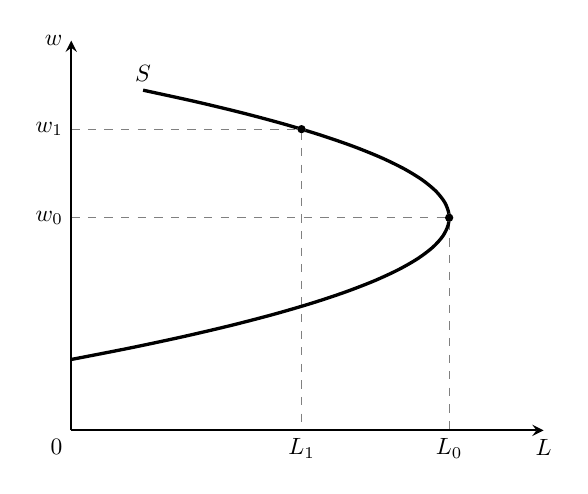
\begin{tikzpicture}[x=1.2cm, y=0.9cm, >=stealth, thick, every node/.style={scale=0.85}]
				% 1. 全局辅助虚线
				\draw[dashed, gray, thin] (0,3) node[left, black] {$w_0$} -- (4,3) -- (4,0) node[below, black] {$L_0$};
				\draw[dashed, gray, thin] (0,4.25) node[left, black] {$w_1$} -- ({-(4.25-3)*(4.25-3)+4},4.25) -- ({-(4.25-3)*(4.25-3)+4},0) node[below, black] {$L_1$};
				
				% 2. 坐标轴
				\draw[->] (0,0) -- (5,0) node[below] {$L$};
				\draw[->] (0,0) -- (0,5.5) node[left] {$w$};
				\node[below left] at (0,0) {$0$};
				
				% 3. 供需实线 (严格裁切定义域至 1.0:4.8，防溢出至第二象限)
				\draw[very thick, domain=1.0:4.8, smooth] plot ({-(\x-3)*(\x-3)+4}, \x);
				\node[above] at ({-(4.8-3)*(4.8-3)+4},4.8) {$S$};
				
				% 4. 交点与标号 (强制白底清除交叉线干扰)
				\fill[white] (4,3) circle (1.5pt); \fill[black] (4,3) circle (1.5pt);
				\fill[white] ({-(4.25-3)*(4.25-3)+4},4.25) circle (1.5pt); \fill[black] ({-(4.25-3)*(4.25-3)+4},4.25) circle (1.5pt);
			\end{tikzpicture}
		\end{center}
		\newpage
		\item \textbf{为什么说一家电脑公司对电脑编程人员的需求是引致需求？}
		
		\textbf{答：}
		引致需求是指由于消费者对最终产品的需求而引起的企业对生产要素的需求，这种需求并非源于直接消费。电脑公司的主要业务是向市场销售电脑以获得利润，而电脑的研发和系统运行则需要雇佣编程人员提供劳务。因此，该公司对编程人员的需求取决于电脑的市场需求。若电脑需求增加，公司就会扩大生产并增加对编程人员的雇佣，反之则减少。
		
		\item \textbf{比较垄断性雇主和竞争性雇主对工人的雇佣选择。哪个会雇佣较多的工人，哪个会支付较高的工资？请解释。}
		
		\textbf{答：}
		竞争性雇主会雇佣更多的工人，并支付更高的工资。这取决于两种市场结构下厂商所面临的劳动力供给条件。在竞争性劳动市场上，单个厂商是工资的接受者，其面临的边际支出与平均支出相等，均等于市场工资水平。垄断性雇主面对整个市场的劳动力供给曲线。由于该曲线向右上方倾斜，雇主若想多雇佣工人就必须提高工资，使得其边际支出始终高于平均支出。
		
		为了实现利润最大化，垄断雇主将边际支出与边际收入产出相等的点确定为最优雇佣量 $L^*$，并在供给曲线上支付对应的更低工资 $w^*$。
		
		由几何关系可知，垄断均衡点位于竞争均衡点 $L_c$ 和 $w_c$ 的左下方。因此，垄断雇主雇佣的工人数量较少，支付的工资水平也较低。
		
		\begin{center}
			\small
			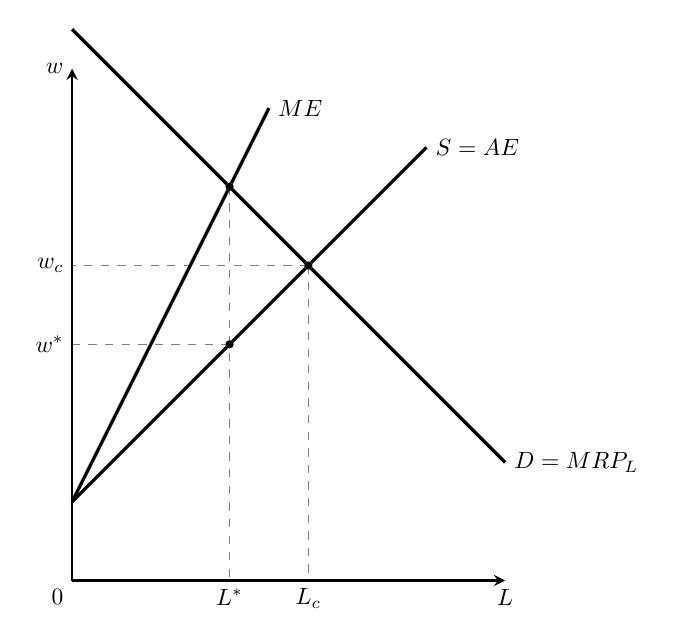
\begin{tikzpicture}[x=1.0cm, y=1.0cm, >=stealth, thick, every node/.style={scale=0.85}]
				% 1. 全局辅助虚线
				\draw[dashed, gray, thin] (2,5) -- (2,0) node[below, black] {$L^*$};
				\draw[dashed, gray, thin] (2,3) -- (0,3) node[left, black] {$w^*$};
				\draw[dashed, gray, thin] (3,4) -- (3,0) node[below, black] {$L_c$};
				\draw[dashed, gray, thin] (3,4) -- (0,4) node[left, black] {$w_c$};
				
				% 2. 坐标轴
				\draw[->] (0,0) -- (5.5,0) node[below] {$L$};
				\draw[->] (0,0) -- (0,6.5) node[left] {$w$};
				\node[below left] at (0,0) {$0$};
				
				% 3. 供需实线
				\draw[domain=0:2.5, smooth, very thick] plot (\x, {1 + 2*\x}) node[right] {$ME$};
				\draw[domain=0:4.5, smooth, very thick] plot (\x, {1 + \x}) node[right] {$S = AE$};
				\draw[domain=0:5.5, smooth, very thick] plot (\x, {7 - \x}) node[right] {$D = MRP_L$};
				
				% 4. 交点与标号
				\fill[white] (2,5) circle (1.5pt); \fill[black] (2,5) circle (1.5pt);
				\fill[white] (2,3) circle (1.5pt); \fill[black] (2,3) circle (1.5pt);
				\fill[white] (3,4) circle (1.5pt); \fill[black] (3,4) circle (1.5pt);
			\end{tikzpicture}
		\end{center}
		
		\item \textbf{摇滚乐手有时能每年挣到好几百万美元的收入。你能用经济租来解释这一大笔收入吗？}
		
		\textbf{答：}
		经济租是指为生产要素实际支付的金额与为获得该要素所必须支付的最低金额之间的差额，其本质是要素稀缺性带来的超额报酬。
		
		在一流摇滚乐手市场上，顶尖人才的供应是极度稀缺且不可替代的。无论市场开价如何，这类乐手的总供给量在短期内几乎固定不变，表现为一条完全无弹性的垂直供给曲线。
		
		由于大众对高质量摇滚音乐的需求极其旺盛，强烈的需求与完全无弹性的供给相结合，直接将均衡价格推向极高水平。
		
		此时，乐手实际获得的巨额报酬中，绝大部分都属于经济租。如果摇滚乐手可以被轻易复制，供给富有弹性，这笔经济租便会大幅缩减。
		
		\begin{center}
			\small
			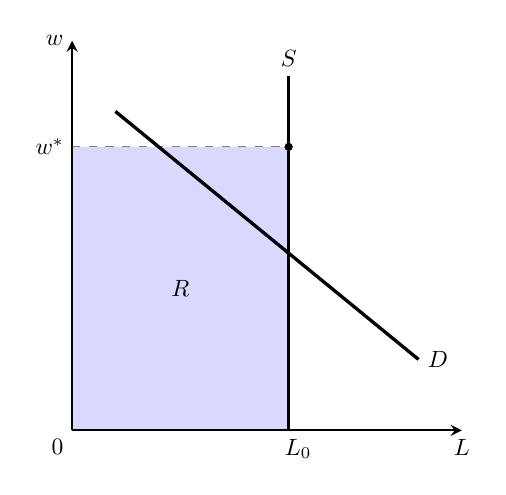
\begin{tikzpicture}[x=1.1cm, y=0.9cm, >=stealth, thick, every node/.style={scale=0.85}]
				% 1. 经济租区域填充 (最底层)
				\fill[blue!15] (0,0) rectangle (2.5,4);
				
				% 2. 全局辅助虚线
				\draw[dashed, gray, thin] (0,4) node[left, black] {$w^*$} -- (2.5,4);
				
				% 3. 坐标轴
				\draw[->] (0,0) -- (4.5,0) node[below] {$L$};
				\draw[->] (0,0) -- (0,5.5) node[left] {$w$};
				\node[below left] at (0,0) {$0$};
				
				% 4. 供需实线 (严格限制在第一象限)
				\draw[very thick] (2.5,0) -- (2.5,5) node[above] {$S$};
				\draw[very thick, domain=0.5:4.0] plot (\x, {5 - \x}) node[right] {$D$};
				
				% 5. 标签与交点
				\node at (1.25,2) {$R$};
				\fill[white] (2.5,4) circle (1.5pt); \fill[black] (2.5,4) circle (1.5pt);
				\node[below, xshift=4pt] at (2.5,0) {$L_0$};
			\end{tikzpicture}
		\end{center}
		
		\item \textbf{当使用的一种投入的互补品增加时，对此投入的需求会出现什么变化？}
		
		\textbf{答：}
		当某种生产投入要素的互补品增加时，对该投入要素的需求将会随之增加。
		
		在生产理论中，两种要素互为互补品意味着它们必须协同发挥作用。当互补投入品（如机器设备）增加时，会直接提高现有要素（如劳动力）的边际产量。
		
		要素边际产量的提升导致其边际收入产出曲线向右上方移动。在要素价格保持不变的前提下，理性的厂商必然会扩大对该要素的雇用规模。
		
		因此，一种要素的雇用量与其互补品的价格呈反方向变动，需求交叉弹性为负，其最终需求量将在互补品增加时显著上升。
		
		\item \textbf{对一个买方垄断购买者来说，一种要素的供给与该要素的边际支出之间是什么关系？}
		
		\textbf{答：}
		对于买方垄断购买者而言，要素的边际支出曲线始终位于该要素的平均支出曲线即供给曲线的上方。
		
		买方垄断者面对的是整个向右上方倾斜的市场要素供给曲线，这意味着厂商若想购买更多的生产要素，就必须为全额要素支付更高的市场价格。
		
		由于厂商必须以统一的更高价格支付给所有已雇用的要素单元，而非仅仅支付给最后追加的那一单位，导致购买要素的边际支出包含了所有存量要素的提价成本。
		
		因此，要素的边际支出必然大于平均支出。在线性供给曲线的条件下，边际支出曲线的斜率正好是平均支出曲线斜率的两倍。
		
		\begin{center}
			\small
			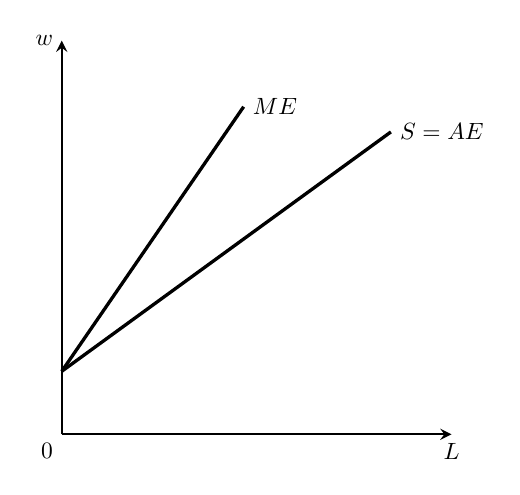
\begin{tikzpicture}[x=1.1cm, y=1.0cm, >=stealth, thick, every node/.style={scale=0.85}]
				% 1. 坐标轴
				\draw[->] (0,0) -- (4.5,0) node[below] {$L$};
				\draw[->] (0,0) -- (0,5.0) node[left] {$w$};
				\node[below left] at (0,0) {$0$};
				
				% 2. 绘图代码（严格限制定义域，防止溢出）
				\draw[very thick, domain=0:3.8, smooth] plot (\x, {0.8 + 0.8*\x}) node[right] {$S = AE$};
				\draw[very thick, domain=0:2.1, smooth] plot (\x, {0.8 + 1.6*\x}) node[right] {$ME$};
			\end{tikzpicture}
		\end{center}
		\newpage
		\item \textbf{目前，全国橄榄球联盟有一项挑选大学球员的制度，它要求一个球员只由一个球队选中，并必须与该球队签约，否则就不能在联盟中踢球。如果这一挑选制度被废除，让所有的球队都能竞争球员，新挑中的球员的工资与资格较老的球员的工资会出现什么情况？}
		
		\textbf{答：}
		现行的单向挑选制度在实质上限制了球员的选择权，使球队所有者联合结成了买方垄断卡特尔，压低了球员的协商薪酬。
		
		一旦该挑选制度被废除，各球队之间为了争夺优秀人才将展开自由竞争，新球员市场将由买方垄断直接转变为完全竞争市场。
		
		在竞争重组后，新挑选球员的工资将大幅上涨，直至等同于其创造的边际收入产出，买方垄断剥蚀租金将不复存在。
		
		相比之下，老球员由于此前已获得自由球员身份，本身就具备较强的市场议价能力并已拿到了市场均衡高薪，因此该制度废除对老球员工资的影响较为有限。
		
		\item \textbf{政府希望鼓励那些靠社会福利救济的人去争取工作。考虑的两种激励计划如下：（1）雇佣靠社会福利救济的人，政府给厂商每人每小时2美元的补贴。（2）对于每家雇佣了一个或多个靠社会救济的人的厂商，政府每年补贴1000美元，而不管雇佣了多少人。每项计划在多大程度上有助于扩大靠社会救济的人的就业机会？}
		
		\textbf{答：}
		厂商雇用工人的决策取决于边际成本与边际收益的博弈。这两项政策在影响厂商的边际雇佣激励上存在本质差异。
		
		计划（1）属于典型的从量边际补贴，使得厂商每多雇用一名福利工人，每小时的有效边际成本就会直接降低2美元。这种机制打破了原有的均衡，促使厂商不断扩大雇用规模，直至工人的边际收入产出下降到与折让后的新边际成本相等，能显著且持续地创造就业机会。
		
		计划（2）属于固定总额补贴，其仅降低了厂商雇用“首个”福利工人时的门槛成本，一旦跨过该门槛，后续多雇工人的边际成本并没有任何改变。
		
		因此，计划（2）缺乏推动厂商进行连续扩产雇佣的边际激励，厂商往往在雇用一名工人拿满津贴后便停止行动，对失业人口整体就业机会的扩大作用远不若计划（1）。
		
		\item \textbf{一家小的专门生产甜饼的企业，唯一的投入变量是劳动，它发现每个工人每天能制作50个甜饼，而成本是每人每天64美元。甜饼的价格是1美元。企业实现了利润最大化吗？试解释。}
		
		\textbf{答：}
		该专门生产甜饼的企业并没有实现利润最大化，其目前的劳动力雇用量规模过大。
		
		根据要素市场的利润最大化原则，厂商雇用劳动力的理性边界应当满足劳动的边际收入产出等于劳动的边际成本。此时该企业的边际经营指标为
		\[
		\begin{aligned}
			MRP_L &= MP_L \cdot P = 50 \times 1 = 50 \text{ 美元/天} \\
			w &= 64 \text{ 美元/天}
		\end{aligned}
		\]
		由于劳动的边际收入产出仅为50美元，明显低于64美元的每日边际出资成本，表明多雇用的工人所带来的追加收益无法弥补其薪酬支出。
		
		因此，该厂商应当缩减工人的雇用数量并削减甜饼产量，通过提升劳动边际产量的方式，使边际收入产出向边际成本靠拢以实现利润最大化。
		\newpage
		\item \textbf{一家企业使用劳动和机器进行生产。试解释为何平均工资率的变化导致了沿着劳动需求曲线的变动，同时也导致了劳动需求曲线本身的移动。}
		
		\textbf{答：}
		平均工资率的变化对要素需求同时存在直接的替代效应和间接的产出效应，分别对应了曲线上的点移动与曲线整体的移动。
		
		当工资率提高时，在其他条件不变的前提下，劳动的相对价格上升，厂商会直接减少劳动的使用量，这表现为沿着既定劳动需求曲线向左上方的点位移动。同时，工资率的普遍上涨会导致企业的边际生产成本曲线整体上移，促使利润最大化的厂商主动缩减合意的最优产出规模。随着整体产出水平的下降，厂商对机器设备等资本投入的需求也会缩减。由于劳动与机器互为生产互补品，资本存量的减少会反过来削弱劳动的边际生产力。
		
		这种生产要素间的互动反馈，最终导致劳动的边际收入产出曲线即劳动需求曲线本身向左方发生整体位移。
		
	\end{enumerate}
	\newpage
	\section{练习题}
	\begin{enumerate}[label=\textbf{\arabic*.}, leftmargin=*]
		\item \textbf{假设工资率是每小时 16 美元，产品价格是 2 美元。每小时产出和劳动投入之间的关系如下：}
		\begin{center}
			\small
			\setlength{\tabcolsep}{12pt}
			\renewcommand{\arraystretch}{1.1}
			\begin{tabular}{cccccccc}
				\hline
				$q$ & 0 & 20 & 35 & 47 & 57 & 65 & 70 \\
				$L$ & 0 & 1  & 2  & 3  & 4  & 5  & 6  \\
				\hline
			\end{tabular}
		\end{center}
		\textbf{（1）找到利润最大化时的劳动数量。（2）假设产品价格保持 2 美元不变，但工资率上升到 21 美元。找到新的利润最大化的劳动数量。（3）假设产品价格增加到 3 美元而工资保持在 16 美元。找到新的利润最大化的劳动数量。（4）假设产品价格 2 美元和工资率 16 美元保持不变，但是技术进步导致任何劳动投入水平下的产出都增加 25\%。找到新的利润最大化的劳动数量。}
		
		\textbf{答：}
		为了进行精确的边际决策，首先根据各阶段的产出增量核算出劳动的边际产量 $MP_L$，并结合产品价格计算出基准状态下的劳动的边际收入产出 $MRP_L$，具体离散分布如下表所示：
		\begin{center}
			\small
			\setlength{\tabcolsep}{10pt}
			\renewcommand{\arraystretch}{1.2}
			\begin{tabular}{ccccccc}
				\hline
				雇用量 $L$ & 1 & 2 & 3 & 4 & 5 & 6 \\
				\hline
				边际产量 $MP_L$ & 20 & 15 & 12 & 10 & 8 & 5 \\
				边际收入产出 $MRP_L (P=2)$ & 40 & 30 & 24 & 20 & 16 & 10 \\
				\hline
			\end{tabular}
		\end{center}
		
		（1）当市场名义工资率 $w_0 = 16$ 美元时，对照上表可知，在劳动雇用量 $L = 5$ 处，工人的边际收入产出恰好等于 16 美元。此时满足要素市场的利润最大化均衡条件 $MRP_L = w$，因此厂商最优的劳动力雇用数量为 5。
		
		（2）当工资率上升至 $w_1 = 21$ 美元时，序列中不存在使 $MRP_L$ 严格等于 21 的整数节点。通过对临界点进行离散总利润 $\pi = P \cdot q - w \cdot L$ 的权衡核算，在 $L = 3$ 时总利润为 $47 \times 2 - 21 \times 3 = 31$ 美元，在 $L = 4$ 时总利润为 $57 \times 2 - 21 \times 4 = 30$ 美元，对比表明雇用 3 名工人时利润最高，故最优劳动数量为 3。
		
		（3）当产品价格上升至 3 美元而工资率维持 16 美元时，各阶段的边际收入产出更替为 $MRP_L = MP_L \cdot 3$，对应序列变为 60、45 Blocks、36、30、24 和 15。此时通过离散利润核算可知，在 $L = 5$ 处的总利润为 $65 \times 3 - 16 \times 5 = 115$ 美元，在 $L = 6$ 处的总利润为 $70 \times 3 - 16 \times 6 = 114$ 美元，因此理性的厂商仍将最优雇用规模锁定为 5。
		
		（4）技术进步使得各阶段的产出全面增幅 25\%，新产出序列对应演化为 25、43.75、58.75、71.25、81.25 和 87.5。在 $P = 2$ 且 $w = 16$ 的约束下，对临界点进行总利润核算，当 $L = 5$ 时企业总利润为 $81.25 \times 2 - 16 \times 5 = 82.5$ 美元，而当 $L = 6$ 时总利润下降为 $87.5 \times 2 - 16 \times 6 = 79$ 美元，由此可确定新的最优劳动力雇用数量仍为 5。
		
		\begin{center}
			\small
			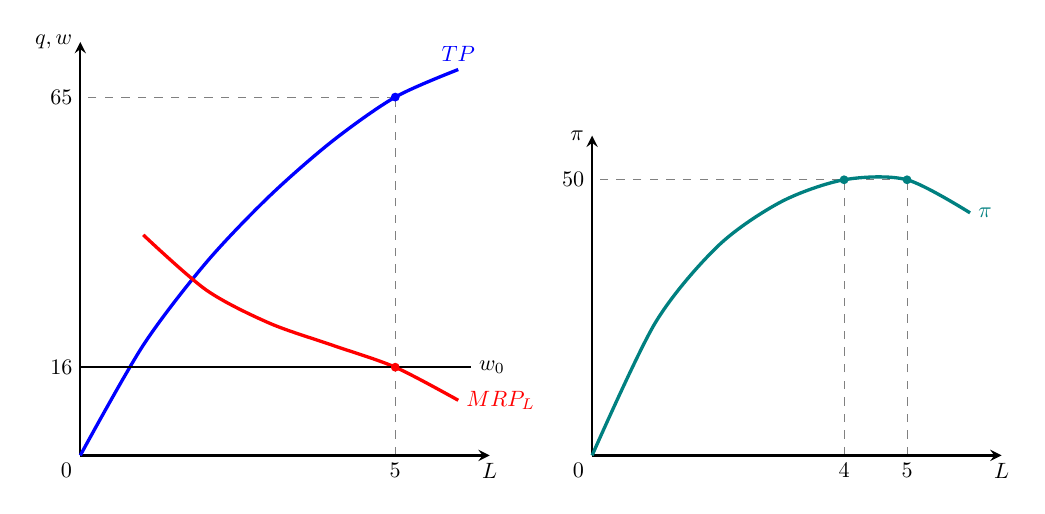
\begin{tikzpicture}[>=stealth, thick, every node/.style={scale=0.80}]
				% ================= 左图：总产量与边际收入产出曲线 =================
				\begin{scope}[x=0.8cm, y=0.07cm]
					% 1. 全局辅助虚线 (精准对应表格离散数据点)
					\draw[dashed, gray, thin] (5,0) node[below, black] {$5$} -- (5,65);
					\draw[dashed, gray, thin] (5,65) -- (0,65) node[left, black] {$65$};
					\draw[dashed, gray, thin] (5,16) -- (0,16) node[left, black] {$16$};
					
					% 2. 坐标轴
					\draw[->] (0,0) -- (6.5,0) node[below] {$L$};
					\draw[->] (0,0) -- (0,75) node[left] {$q, w$};
					\node[below left] at (0,0) {$0$};
					
					% 3. 曲线绘制 (使用 plot coordinates 确保曲线绝对穿过数据点)
					\draw[very thick, color=blue, smooth] plot coordinates {
						(0,0) (1,20) (2,35) (3,47) (4,57) (5,65) (6,70)
					}; 
					\node[above, blue] at (6,70) {$TP$};
					
					\draw[very thick, color=red, smooth] plot coordinates {
						(1,40) (2,30) (3,24) (4,20) (5,16) (6,10)
					};
					\node[right, red] at (6,10) {$MRP_L$};
					
					% 工资率水平线
					\draw[thick, color=black] (0,16) -- (6.2,16) node[right] {$w_0$};
					
					% 4. 关键交点实心化
					\fill[blue] (5,65) circle (1.6pt);
					\fill[red] (5,16) circle (1.6pt);
				\end{scope}
				
				% ================= 右图：总利润曲线 (xshift压缩至6.5cm防溢出) =================
				\begin{scope}[x=0.8cm, y=0.07cm, xshift=6.5cm]
					% 1. 全局辅助虚线 (精准展示 L=4 与 L=5 的双顶点达峰特征)
					\draw[dashed, gray, thin] (4,0) node[below, black] {$4$} -- (4,50);
					\draw[dashed, gray, thin] (5,0) node[below, black] {$5$} -- (5,50);
					\draw[dashed, gray, thin] (5,50) -- (0,50) node[left, black] {$50$};
					
					% 2. 坐标轴
					\draw[->] (0,0) -- (6.5,0) node[below] {$L$};
					\draw[->] (0,0) -- (0,58) node[left] {$\pi$};
					\node[below left] at (0,0) {$0$};
					
					% 3. 总利润曲线绘制
					\draw[very thick, color=teal, smooth] plot coordinates {
						(0,0) (1,24) (2,38) (3,46) (4,50) (5,50) (6,44)
					};
					\node[right, teal] at (6,44) {$\pi$};
					
					% 4. 利润最高点标记
					\fill[teal] (4,50) circle (1.6pt);
					\fill[teal] (5,50) circle (1.6pt);
				\end{scope}
			\end{tikzpicture}
		\end{center}
		
		
		\newpage
		\item \textbf{假定那些收入低于 10000 美元的工人目前不必缴纳联邦所得税。假定一项新的政府计划保证给工人 5000 美元，无论他有没有任何收入，对于所有得到的收入，达到 10000 美元，工人就必须向政府缴纳 50\% 的税。画出在这新计划下工人面临的预算线。这一计划可能如何影响工人的劳动供给？}
		
		\textbf{答：}
		新福利计划的推行使低收入工人的消费与闲暇预算约束线发生了分段偏转。在新计划实施前，由于自产收入低于 10000 美元时免税，工人的初始预算线是一条斜率绝对值为名义工资率 $w$ 的完整直线。
		
		新计划实施后，若工人完全不工作，仍可获得 5000 美元的无条件保障金，这导致闲暇轴交点垂直上移。在自产收入达到 10000 美元之前的低收入区间，由于面临 50\% 的边际税率，预算线的斜率绝对值折半减降为 $0.5w$。
		
		当自产收入达到 10000 美元时，工人累计缴纳的税收恰好为 5000 美元，与政府发放的保障金完全抵消。因此，在自产收入超过 10000 美元的高收入区间，新预算线与原预算线完全重合，不再发生任何平移。
		
		这一政策调整对原先收入低于 10000 美元的基层劳动者具有显著的负向劳动激励。5000 美元的兜底财富带来了倾向于增加闲暇的收入效应，而 50\% 的高边际税率则大幅降低了闲暇的机会成本，其替代效应同样促使劳动供给减少。在两种效应的同向共振下，这些工人将会明显缩短工作时间。
		
		\begin{center}
			\small
			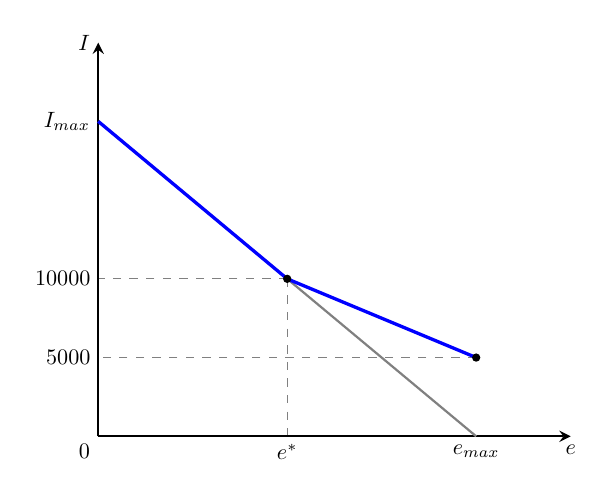
\begin{tikzpicture}[x=1.2cm, y=1.0cm, >=stealth, thick, every node/.style={scale=0.80}]
				% 1. 全局辅助虚线 (精准对齐，绝无交叉干扰)
				\draw[dashed, gray, thin] (4,1) -- (0,1) node[left, black] {5000};
				\draw[dashed, gray, thin] (2,2) -- (2,0) node[below, black] {$e^*$};
				\draw[dashed, gray, thin] (2,2) -- (0,2) node[left, black] {10000};
				
				% 2. 坐标轴
				\draw[->] (0,0) -- (5.0,0) node[below] {$e$};
				\draw[->] (0,0) -- (0,5.0) node[left] {$I$};
				\node[below left] at (0,0) {$0$};
				
				% 3. 原始预算线
				\draw[thick, gray, domain=0:4] plot (\x, {4 - \x});
				\node[left] at (0,4) {$I_{max}$};
				\node[below] at (4,0) {$e_{max}$};
				
				% 4. 新预算线 (分段绘制，在 (2,2) 处与原线完美接轨并重合)
				\draw[very thick, color=blue, domain=2:4] plot (\x, {3 - 0.5*\x});
				\draw[very thick, color=blue, domain=0:2] plot (\x, {4 - \x});
				
				% 5. 关键政策均衡点标记
				\fill[black] (2,2) circle (1.5pt);
				\fill[black] (4,1) circle (1.5pt);
			\end{tikzpicture}
		\end{center}
		
		\item \textbf{利用你关于边际产出收益的知识，解释下列现象：（1）一个著名的网球明星在一个 30 秒钟的电视商业片中得到 20 万美元酬金。而那个扮演搭档的演员只得到 500 美元。（2）为了让一个经营不善的储蓄贷款机构的总裁放弃最后两年的合同，向他付钱。（3）一架载客 400 人的大型喷气客机比载客 250 人的客机定价高，即使两种飞机的制造成本是相同的。}
		
		\textbf{答：}
		（1）要素市场的均衡报酬是由要素的边际收入产出决定的。顶级网球明星由于具备极高的社会知名度与粉丝号召力，能够为广告品牌注入庞大的市场关注度并直接拉动产品销量，其边际收入产出极其巨大。相比之下，普通的搭档演员仅起到背景烘托作用，其在广告收益中的边际贡献微乎其微，因而两者的酬金差距完全符合要素定价的基本规律。
		
		（2）经营不善的储蓄贷款机构总裁由于决策失误或管理无方，其留在现任岗位上继续运营企业所带来的边际收入产出在实质上已经演变为负值。在此情形下，董事会通过支付一笔买断费使其提前离职，并引入更有能力的继任者，能够有效及时地阻断亏损扩大，这种“花钱请人走”的策略从边际决策视角审视是完全理性且能挽回企业长期价值的。
		
		（3）客机作为航空公司的生产要素，其带来的边际收益直接取决于其单次航行的最大载客周转量。400 人座的大型喷气客机在航线运营中能够成倍地提高单次航班的机票总收入，其创造的要素边际收入产出远高于 250 人座的客机。虽然两者的工厂制造成本可能完全一致，但航空公司愿意为其支付的要素买标价格只取决于其未来所能派生的收益流大小。
		
		\item \textbf{如果对下列生产要素的需求增加了，对相关消费品的需求会如何变化？如果对消费品的需求保持不变，对这些生产要素的引致需求的增加有哪些可能解释呢？（1）计算机内存；（2）客机用航空燃料；（3）新闻用纸；（4）饮料罐用的铝。}
		
		\textbf{答：}
		（1）若计算机内存需求增加，通常意味着下游计算机消费市场的总体需求也出现了同向扩张。如果在最终计算机产品需求保持不变的背景下内存需求依然上升，其合理的替代解释在于，由于组装技术调整或其余元器件（如处理器）的相对价格出现大幅下降，引致了计算机整体供给规模的扩张，从而连带提振了对核心内存要素的派生需求。
		
		（2）航空燃料在民航运输服务中具有极强的不可替代性，其需求上涨往往直接对应着终端旅客对航空出行服务消费的长足增长。如果在民航客运需求维持静态不变的条件下燃料使用量增加，其可能的原因在于其他互补或相关要素（例如空乘地勤人员薪资或机场起降规费）出现下调，降低了航空公司的边际运营成本并促使其增开航线，从而诱发了航空燃料的增量消费。
		
		（3）新闻用纸的需求上涨一般直接映射了报纸及纸质传媒市场订阅需求的景气扩张。若消费端的报纸需求处于完全恒定的状态，则纸张要素引致需求增加的经济学动因在于印刷油墨、报业投递人工等其余协同生产要素的价格发生大幅下跌，这使得报社的供给能力在成本驱动下发生右移，从而在较低的报纸市价下撬动了更多的新闻纸消耗。
		
		（4）饮料罐用铝材引致需求的急剧上升，在通常情况下直接派生于快消品或软饮料消费市场的季节性需求爆发。如果在终端软饮料需求并未发生任何波动的常态下铝材消耗依旧上涨，则最可信的经济学解释包括：一是玻璃、塑料等相互替代的包装容器材料在市场上出现了大幅提价；二是再生铝或新型加工工艺的使用提高了铝罐包装的边际性价比，引发了材料间的跨替代效应。
		
		\item \textbf{假定有两组工人，加入工会的和未加入工会的。国会通过一项法律，要求所有工人参加工会。你预期以前没有加入工会的工人和原来已加入工会的工人的工资率会出现什么情况？你是如何假设工会的行为的？}
		
		\textbf{答：}
		法律强制要求全民加入工会后，预期以前未加入工会的工人工资率会上升，而原来已加入工会的工人工资率可能保持不变或发生下降。
		
		对工会行为的假设是，工会作为一个具有强市场垄断势力的独占卖方，能够通过集体谈判控制劳动力供给并选择目标工资率。其核心决策取决于工会的福利目标，即在最大化成员名义工资与最大化整体就业率之间进行边际权衡。
		
		对于以前未加入工会的工人，法律使其获得了工会垄断势力的庇护，资方无法再用廉价的非工会劳动力对其进行替代，因此其谈判工资必然随之大幅度上涨。
		
		然而，由于全员加入导致工会内部的劳动力总供给规模显著扩张，工会必须设法吸纳这部分新增成员就业。面对向下倾斜的劳动力需求曲线，若要维持原有的高工资，势必导致大量新成员失业；若要保障整体就业率，工会就必须在集体谈判中向资方让步，调低其名义工资标准，从而导致原有工会成员的工资面临下行压力。
		\newpage
		\item \textbf{假定厂商的生产函数是 $Q = 12L - L^2$，$L = 0 \sim 6$，其中 $L$ 是每天的劳动投入，$Q$ 是每天的产出。如果产出品在竞争性市场上以 10 美元出售，导出并画出厂商的劳动需求曲线。当工资率为每天 30 美元时，厂商将雇佣多少工人？工资率为每天 60 美元呢？}
		
		\textbf{答：}
		在完全竞争的产品市场上，厂商面对的产品价格等于其边际收益，即 $P = MR = 10$ 美元。通过对生产函数求导，可得劳动的边际产量函数为
		\[
		MP_L = \frac{\text{d}Q}{\text{d}L} = 12 - 2L
		\]
		厂商对劳动的需求曲线由劳动的边际收入产出决定。将其展开可导出劳动的需求函数关系式为
		\[
		MRP_L = MR \cdot MP_L = 10 \times (12 - 2L) = 120 - 20L
		\]
		根据利润最大化原则，厂商雇用劳动力的边际边界应满足 $MRP_L = w$。当市场工资率 $w = 30$ 美元时，代入联立方程 $120 - 20L = 30$，解得最优劳动雇用量 $L = 4.5$。
		
		同理，当市场工资率上涨至 $w = 60$ 美元时，代入要素均衡条件 $120 - 20L = 60$，解得此时的最优劳动雇用量缩减为 $L = 3$。
		
		\begin{center}
			\small
			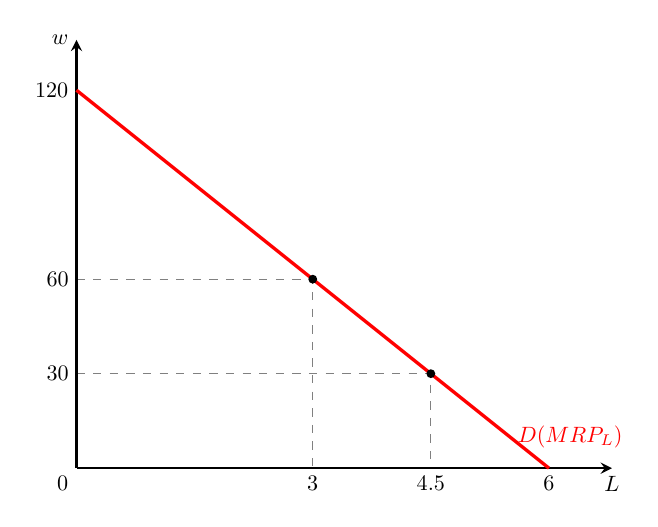
\begin{tikzpicture}[x=1.0cm, y=0.8cm, >=stealth, thick, every node/.style={scale=0.80}]
				% 1. 全局辅助虚线 (纵轴数值除以20进行等比例降维映射，防止溢出)
				\draw[dashed, gray, thin] (0,3) node[left, black] {$60$} -- (3,3) -- (3,0) node[below, black] {$3$};
				\draw[dashed, gray, thin] (0,1.5) node[left, black] {$30$} -- (4.5,1.5) -- (4.5,0) node[below, black] {$4.5$};
				
				% 2. 坐标轴
				\draw[->] (0,0) -- (6.8,0) node[below] {$L$};
				\draw[->] (0,0) -- (0,6.8) node[left] {$w$};
				\node[below left] at (0,0) {$0$};
				\node[left] at (0,6) {$120$};
				\node[below] at (6,0) {$6$};
				
				% 3. 需求曲线实线 (严格限制在第一象限)
				\draw[very thick, color=red, domain=0:6] plot (\x, {6 - \x});
				\node[right, red] at (5.5,0.5) {$D(MRP_L)$};
				
				% 4. 关键均衡点标记
				\fill[black] (3,3) circle (1.6pt);
				\fill[black] (4.5,1.5) circle (1.6pt);
			\end{tikzpicture}
		\end{center}
		
		\item \textbf{在美国，士兵的唯一合法雇主是联邦政府。如果政府利用自己的买方垄断者的地位，在估计征募多少士兵时，将会制定什么标准？如果实行义务兵役制会怎样？}
		
		\textbf{答：}
		作为募兵市场上的唯一合法雇主，联邦政府具有典型的买方垄断势力。其在评估征募士兵规模时，制定的最优化标准是使雇用士兵的边际支出等于士兵的边际收入产出。
		
		由于买方垄断下厂商面对向右上方倾斜的劳动力供给曲线，多募兵员会导致存量兵员的薪资整体上升，因而政府招募士兵的边际支出线始终高于平均支出线。这导致联邦政府最终确定的征兵规模和支付的军人工资，均显著低于完全竞争市场结构下的均衡水平。
		
		若国家转而实行强征性的义务兵役制，劳动力供给的法律约束将彻底打破原有的市场均衡。此时，政府获得了以极低法定工资强制征召任意数量兵员的绝对行政权力。
		
		在义务兵役制下，由于普通应征士兵失去了在市场上自由议价和放弃工作的权利，专业军人的平均工资水平将会被迫压低，而国家整体征募和保有防务的士兵数量则会大幅度扩张。
		\newpage
		\item \textbf{一行业对劳动的需求由曲线 $L = 1200 - 10w$ 给出，其中 $L$ 是每天的劳动需求，$w$ 是工资率。供给曲线由 $L = 20w$ 给出。均衡工资率和雇佣的劳动数量是多少？工人得到的经济租金是多少？}
		
		\textbf{答：}
		要素市场实现竞争均衡时，劳动力的市场需求量与市场供给量相等。联立劳动供求方程组
		\[
		\begin{cases}
			L = 1200 - 10w \\
			L = 20w
		\end{cases}
		\]
		解得要素市场的均衡名义工资率为 $w^* = 40$ 美元，均衡劳动雇用数量为 $L^* = 800$。
		
		经济租金是指要素所有者实际获得的报酬与为其吸引该要素完成供给所必需的最低报酬之间的差额。在几何图景中，其精确对应于市场均衡工资线以下、要素供给曲线以上的三角形闭合区域面积。
		
		将供给曲线改写为反供给函数形式可得 $w = L / 20$。根据三角形面积公式，工人们在均衡状态下所累计获得的经济租金总额为
		\[
		\text{经济租金} = \frac{1}{2} \times w^* \times L^* = \frac{1}{2} \times 40 \times 800 = 16000 \text{ 美元}
		\]
		
		\begin{center}
			\small
			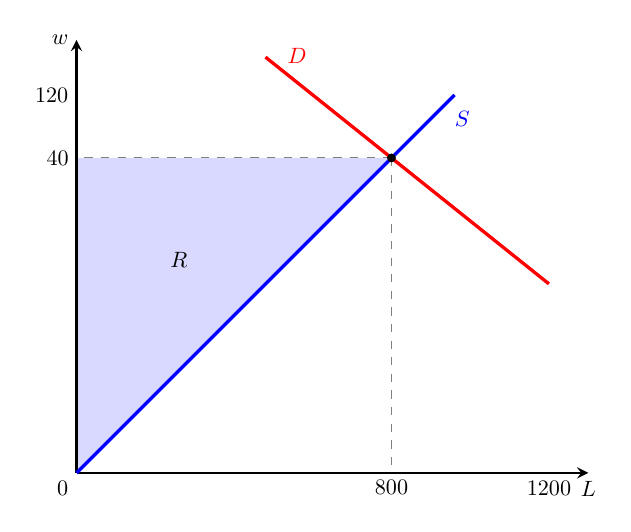
\begin{tikzpicture}[x=1.0cm, y=1.0cm, >=stealth, thick, every node/.style={scale=0.80}]
				% 1. 经济租金区域填充 (最底层)
				\fill[blue!15] (0,0) -- (4,4) -- (0,4) -- cycle;
				
				% 2. 全局辅助虚线 (横轴除以200，纵轴除以10进行降维无损映射)
				\draw[dashed, gray, thin] (4,4) -- (4,0) node[below, black] {$800$};
				\draw[dashed, gray, thin] (4,4) -- (0,4) node[left, black] {$40$};
				
				% 3. 坐标轴
				\draw[->] (0,0) -- (6.5,0) node[below] {$L$};
				\draw[->] (0,0) -- (0,5.5) node[left] {$w$};
				\node[below left] at (0,0) {$0$};
				\node[left] at (0,4.8) {$120$};
				\node[below] at (6,0) {$1200$};
				
				% 4. 供需实线
				\draw[very thick, color=blue, domain=0:4.8] plot (\x, {\x});
				\node[right, blue] at (4.7,4.5) {$S$};
				
				\draw[very thick, color=red, domain=2.4:6] plot (\x, {4.8 - 0.8*(\x - 3)});
				\node[above, red] at (2.8,5.1) {$D$};
				
				% 5. 均衡点与内部标签
				\fill[black] (4,4) circle (1.6pt);
				\node at (1.3,2.7) {$R$};
			\end{tikzpicture}
		\end{center}
		
		\item \textbf{利用第8题中的信息。现在假定唯一可得的劳动由一个垄断性工会控制，它希望使工会成员得到的经济租最大化。被雇佣的劳动数量和工资率将是多少？你的答案如何与第8题的答案进行比较？请讨论。（提示：工会的边际收益曲线由 $MR = 120 - 0.2L$ 给定。）}
		
		\textbf{答：}
		垄断工会若以最大化全体成员的经济租金为目标，其行为类似于产品市场上的垄断厂商。工会不仅要追求总名义工资收入，还必须扣除出让闲暇的机会成本，因此其边际决策准则为要素边际收益等于劳动力供给价格。
		
		联立需求派生的边际收益函数与市场劳动力供给函数 $w = L / 20$，可得租金最大化的要素边界条件为 $120 - 0.2L = 0.05L$。解得工会最优限制的劳动雇用数量为 $L^* = 480$。此时，工人的最低保留工资即机会成本为 $w_s = 480 / 20 = 24$ 美元。
		
		由于工会垄断了要素供给，它可以强行迫使买方企业沿着劳动力需求曲线进行雇用。将最优雇用量 480 代入反需求函数 $w = 120 - 0.1L$ 中，最终确定的市场名义工资率为 $w^* = 72$ 美元。
		
		此时工会成员累计获得的经济租金在几何上表现为工资线以下、供给曲线以上的闭合区域面积。通过梯形面积公式核算，总经济租金为 $(72 - 24) \times 480 + 0.5 \times 24 \times 480 = 28800$ 美元。
		
		与第8题的完全竞争市场均衡（$L_c = 800, w_c = 40$）对比可知，工会通过行使买方垄断势力，主动限制了近 40\% 的劳动力就业机会。这种“控量抬价”的垄断策略成功将市场工资率由 40 美元大幅拉升至 72 美元，并实现了经济租金的极值化。
		
		\begin{center}
			\small
			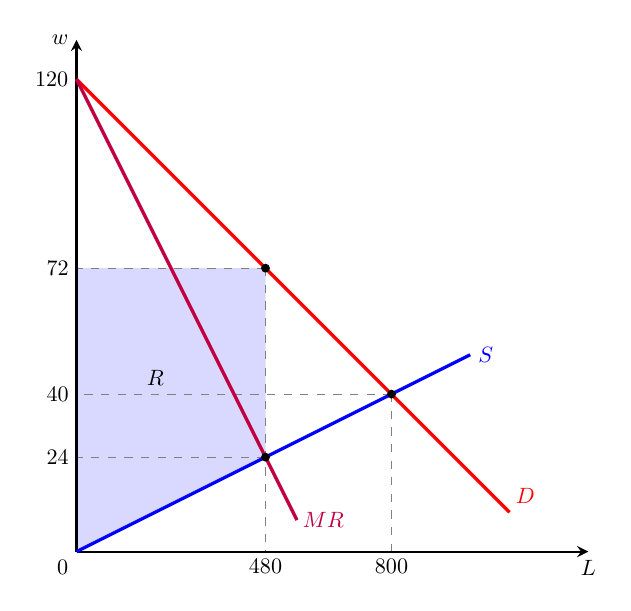
\begin{tikzpicture}[x=1.0cm, y=1.0cm, >=stealth, thick, every node/.style={scale=0.80}]
				% 1. 经济租金区域填充 (最底层)
				\fill[blue!15] (0,0) -- (2.4,1.2) -- (2.4,3.6) -- (0,3.6) -- cycle;
				
				% 2. 全局辅助虚线 (横轴除以200，纵轴除以20进行降维映射)
				\draw[dashed, gray, thin] (2.4,3.6) -- (2.4,0) node[below, black] {$480$};
				\draw[dashed, gray, thin] (2.4,3.6) -- (0,3.6) node[left, black] {$72$};
				\draw[dashed, gray, thin] (2.4,1.2) -- (0,1.2) node[left, black] {$24$};
				\draw[dashed, gray, thin] (4,2) -- (4,0) node[below, black] {$800$};
				\draw[dashed, gray, thin] (4,2) -- (0,2) node[left, black] {$40$};
				
				% 3. 坐标轴
				\draw[->] (0,0) -- (6.5,0) node[below] {$L$};
				\draw[->] (0,0) -- (0,6.5) node[left] {$w$};
				\node[below left] at (0,0) {$0$};
				\node[left] at (0,6) {$120$};
				
				% 4. 供需与边际线条 (精准切除多余定义域)
				\draw[very thick, color=blue, domain=0:5] plot (\x, {0.5*\x});
				\node[right, blue] at (5,2.5) {$S$};
				
				\draw[very thick, color=red, domain=0:5.5] plot (\x, {6 - \x});
				\node[above, red] at (5.7,0.5) {$D$};
				
				\draw[very thick, color=purple, domain=0:2.8] plot (\x, {6 - 2*\x});
				\node[left, purple] at (3.5,0.4) {$MR$};
				
				% 5. 关键点与内部租金标签
				\fill[black] (4,2) circle (1.6pt);
				\fill[black] (2.4,3.6) circle (1.6pt);
				\fill[black] (2.4,1.2) circle (1.6pt);
				\node at (1.0,2.2) {$R$};
			\end{tikzpicture}
		\end{center}
		
		\item \textbf{一个企业以劳动作为单一投入，产出为 $q$，生产函数为 $q = 8L^{1/2}$。商品售价是 150 美元/单位，工资率是 75 美元/小时。（1）找出利润最大化时的 $L$ 数量。（2）找出利润最大化时的 $q$ 数量。（3）最大利润是多少？（4）假设现在每单位的产出要征税 30 美元，而每小时的劳动能得到 15 美元的补助。并且假设企业是价格接受者，产品价格保持 150 美元不变。找出新的利润最大化的 $L$、$q$ 和利润。（5）假设企业要为利润支付 20\% 的税额。找出新的利润最大化的 $L$、$q$ 和利润。}
		
		\textbf{答：}
		（1）由于企业处于完全竞争的产品与要素市场中，其初始的总收益为 $150 \times 8L^{1/2}$，总成本为 $75L$。构建其利润函数并对劳动要素求一阶导数，可得利润最大化的边际条件为
		\[
		\frac{\text{d}\pi}{\text{d}L} = 600L^{-1/2} - 75 = 0
		\]
		解得利润最大化时的最优劳动需求数量为 $L = 64$ 小时。
		
		（2）将最优劳动投入量 $L = 64$ 代入企业生产函数中，可以直接求得利润最大化条件下的最优总产量为 $q = 8 \times \sqrt{64} = 64$ 单位。
		
		（3）将最优要素投入与均衡产量代入利润恒等式中，企业能实现的最大化经济利润为 $\pi = 150 \times 64 - 75 \times 64 = 4800$ 美元。
		
		（4）在引入政府调控政策后，扣除从量税后的净产品售价下降为 $150 - 30 = 120$ 美元，而获得补贴后的实际净要素工资率降为 $75 - 15 = 60$ 美元。此时构建新环境下的利润函数并求导
		\[
		\frac{\text{d}\pi'}{\text{d}L} = 120 \times 4L^{-1/2} - 60 = 480L^{-1/2} - 60 = 0
		\]
		解得新政策约束下的最优劳动数量仍为 $L = 64$ 小时，对应的总产量保持 $q = 64$ 单位不变。此时企业的最终净利润缩减为 $\pi' = 120 \times 64 - 60 \times 64 = 3840$ 美元。
		
		（5）当政府针对企业的纯经济利润征收 20\% 的比例所得税时，企业的目标函数转化为最大化税后净利润。由于比例税不改变一阶导数归零的决策位置，其具体的数理结构为
		\[
		\frac{\text{d}\pi''}{\text{d}L} = 0.8 \times \left( 600L^{-1/2} - 75 \right) = 480L^{-1/2} - 60 = 0
		\]
		经求解可知，在纯利润税制度下，企业的最优决策同样维持 $L = 64$ 小时及 $q = 64$ 单位不变，留存的税后净利润为 $\pi'' = 4800 \times (1 - 0.2) = 3840$ 美元。这表明第（4）问的结构性税补组合与第（5）问的利润税在生产行为上具有完全相同的行为中性特征。
		
	\end{enumerate}
	
	% =======================================================
	%                 第 15 章：投资、时间与资本市场
	% =======================================================
	\chapter{投资、时间与资本市场}
	
	\section{复习题}
	\begin{enumerate}[label=\textbf{\arabic*.}, leftmargin=*]
		\item \textbf{一个厂商用布和劳动作为投入要素生产衬衫，工厂是用 1000 万美元买来的。这些投入要素中哪些是以流量衡量的，哪些是以存量衡量的？如果该厂商不是购买而是租赁了该工厂，你的回答会如何？它的产出是以流量还是存量衡量？它的利润呢？}
		
		\textbf{答：}
		存量是在特定时点上衡量的数量，而流量是在一段时间内衡量的数量。
		厂商购买的价值 1000 万美元的工厂属于在特定时点资产的沉淀，是以存量衡量的资本。
		布和劳动作为生产过程中的持续投入，是针对一段特定生产周期而言的，因而以流量衡量。
		
		如果厂商改为租赁工厂，租赁费作为一段时期内发生的资本服务支出，工厂的使用成本便转化为流量衡量。
		无论是购买还是租赁工厂，企业的产出和利润都是在一定时期内创造和结算的，因此它们始终以流量衡量。
		
		\item \textbf{投资者如何计算一种债券的净现值？如果利率是 $5\%$ ，每年支付 1000 美元的永久债券的现值是多少？}
		
		\textbf{答：}
		债券的净现值通过将未来所有预期的利息支付和最终本金偿还，按市场贴现率折算为当前时点的价值并求和得到。
		一种每年支付 $W$ 元利息、期限为 $n$ 年且到期偿还本金 $M$ 的债券，其现值计算公式为
		\[
		\text{PDV} = \frac{W}{1+R} + \frac{W}{(1+R)^2} + \dots + \frac{W}{(1+R)^n} + \frac{M}{(1+R)^n}
		\]
		式中，$R$ 代表市场贴现率。
		
		永久债券承诺无限期地每年支付固定利息，由于其没有到期日，不存在最终的本金偿还。
		通过对无限项等比数列求和，永久债券的现值公式可以简化为
		\[
		\text{PDV} = \frac{W}{R}
		\]
		当市场利率为 $5\%$，年利息为 1000 美元时，该永久债券的现值计算为
		\[
		\text{PDV} = \frac{1000}{0.05} = 20000 \text{（美元）}
		\]
		
		\item \textbf{债券的有效收益率是什么？如何计算它？为什么有些公司债券的有效收益率比另一些公司债券高？}
		
		\textbf{答：}
		有效收益率是使债券未来所有预期支付流量的现值，恰好等于当前债券市场价格的贴现率。
		对于每年支付 $W$ 元利息、市场价格为 $P$ 的永久债券，其有效收益率 $R$ 可直接通过价格公式逆运算求得
		\[
		R = \frac{W}{P}
		\]
		对于一般的 $n$ 年期期末还本债券，若市场价格为 $P$，其有效收益率 $R$ 需通过求解如下方程得到
		\[
		P = \frac{W}{1+R} + \frac{W}{(1+R)^2} + \dots + \frac{W}{(1+R)^n} + \frac{M}{(1+R)^n}
		\]
		
		不同公司债券的有效收益率存在差异，其核心原因在于债券发行主体的违约风险不同。
		财务状况较弱、信用评级较低的公司，其债券发生违约的可能性更大。
		为了吸引风险厌恶型的投资者，这些公司必须提供更高的风险溢价，从而导致其债券具有较高的有效收益率。
		
		\item \textbf{投资决策的净现值标准是什么？如何计算投资项目的净现值？如果该项目的所有现金流量都是确定的，应当用什么样的贴现率来计算净现值？}
		
		\textbf{答：}
		投资决策的净现值标准规定，只有当一个投资项目未来所有预期现金流量的现值之和大于该项目的初始投资成本时，厂商才应当进行投资。
		若项目的初始资本投资成本为 $C$，未来 $n$ 年内预计产生的利润流量分别为 $\pi_1, \pi_2, \dots, \pi_n$，则净现值的计算公式为
		\[
		\text{NPV} = -C + \frac{\pi_1}{1+R} + \frac{\pi_2}{(1+R)^2} + \dots + \frac{\pi_n}{(1+R)^n}
		\]
		式中，$R$ 代表资本的机会成本，即投资于该项目所放弃的同等风险其他资产的回报率。
		
		如果该项目的所有现金流量在未来都是完全确定的，这意味着该投资项目不存在任何经营与财务风险。
		此时，该项目的机会成本应当等于市场上无风险资产的回报率。
		因此，计算该净现值时应当采用无风险利率，在实际应用中通常参照政府公债或国库券的利率。
		
		\item \textbf{你退休了并且有两种选择：一是可以从公司拿到一次性支付；二是接受一个你在有生之年每年都会支付给你的较小的年金。你的哪种决策将是最优的？你需要什么信息？}
		
		\textbf{答：}
		最优的决策取决于哪种选择能够带来更高的现值。一次性支付的现值即为其当前的总金额，而年金的现值需要将未来的现金流折现。
		为了做出理性决策，退休者需要评估自身的预期寿命，从而确定年金支付的持续期数。
		同时，还需要了解当前的金融市场利率或个人资产投资的预期回报率，以此作为折现年金流的贴现率。
		
		此外，决策者还必须考虑自身的风险偏好以及资金管理能力。
		年金能够有效规避因寿命超出预期而导致资金耗尽的生存风险，提供稳定的消费保障。
		若选择一次性支付，虽然资金灵活性更高，但退休者需要独自承担市场投资风险与长期的资金管理负担。
		
		\item \textbf{你注意到了过去几个月里债券价格的上升。这意味着利率发生了怎样的变化？试解释。}
		
		\textbf{答：}
		债券价格的上升意味着市场利率已经下降。可以用最基础的永久债券定价公式来直观呈现这一反向变动关系
		\[
		P = \frac{C}{R}
		\]
		式中，$P$ 为债券市场价格，$C$ 为固定的年票息，$R$ 为市场利率。
		
		通过对市场利率求导，可以清晰地看到价格对利率的敏感度
		\[
		\frac{dP}{dR} = -\frac{C}{R^2} < 0
		\]
		该导数恒小于零，在数学上证明了债券价格与市场利率之间必然存在着反向变动机制。
		
		当市场利率下降时，由于未来固定票息流的贴现率变低，现值随之提高，从而在市场上表现为当前的债券价格上升。
		债券价格会持续调整，直至其蕴含的有效收益率重新与下降后的市场利率达成跨期套利均衡。
		\newpage
		\item \textbf{实际贴现率与名义贴现率之间的区别是什么？什么时候应当用实际贴现率来计算净现值？什么时候应当用名义贴现率？}
		
		\textbf{答：}
		实际贴现率与名义贴现率的核心区别在于是否剔除了通货膨胀因子的干扰。两者的基本数理关系可以通过费雪方程式来表达
		\[
		R_n = R_r + \pi^e
		\]
		式中，$R_n$ 为名义贴现率，$R_r$ 为实际贴现率，$\pi^e$ 为预期的通货膨胀率。
		
		在计算投资项目的净现值时，贴现率的选择必须与未来现金流量的估算口径保持绝对的数学对称
		\[
		\text{NPV} = \sum_{t=1}^n \frac{\text{名义现金流}_t}{(1+R_n)^t} = \sum_{t=1}^n \frac{\text{实际现金流}_t}{(1+R_r)^t}
		\]
		
		如果未来的预期现金流量是以剔除通胀后的实际购买力计量的，就必须采用实际贴现率 $R_r$ 进行折现。
		反之，如果现金流量是以包含通胀因素的名义货币额计量的，则必须采用名义贴现率 $R_n$。只要遵循口径一致性原则，两种计算方法得到的净现值结果完全相同。
		
		\item \textbf{风险溢价是如何用来补偿净现值计算中的风险的？可分散风险与不可分散风险有什么不同？为什么只有不可分散风险应当包括在风险溢价内？}
		
		\textbf{答：}
		风险溢价通过在无风险利率之上进行数学加成，从而系统性地提高了净现值计算中所使用的风险调整贴现率
		\[
		R = R_f + R_p
		\]
		式中，$R$ 为风险调整贴现率，$R_f$ 为无风险利率，$R_p$ 为风险溢价。
		
		将该贴现率代入项目的净现值公式中，可以清晰地看到其对高风险现金流的风险惩罚机制
		\[
		\text{NPV} = -C + \sum_{t=1}^n \frac{\mathbb{E}(\pi_t)}{(1 + R_f + R_p)^t}
		\]
		式中，$\mathbb{E}(\pi_t)$ 为未来的预期利润。较大的风险溢价 $R_p$ 会增大分母，从而理性下调高风险资产的现值。
		
		可分散风险可以通过持有资产组合消除，而不可分散风险由宏观系统性因素决定，无法通过多元化投资化解。
		由于投资者可以通过构建组合无成本地消除特质性风险，资本市场不会对可分散风险提供任何超出无风险利率的额外报酬。
		只有不可分散风险无法被稀释，构成了投资者承担的实质性资产机会成本，因此必须将其定量化为风险溢价 $R_p$ 并纳入贴现率中。
		
		\item \textbf{资本资产定价模型中的“市场回报率”是什么意思？为什么该市场回报率高于无风险利率？资本资产定价模型中一项资产的 $\beta$ 值衡量什么？为什么高 $\beta$ 值资产的预期回报率应比低 $\beta$ 值资产高？}
		
		\textbf{答：}
		在资本资产定价模型中，市场回报率是指投资者购买了由整个股票市场所有资产构成的风险组合时，所能获得的预期收益率。
		该模型的经典线性均衡方程为
		\[
		r_i = r_f + \beta_i (r_m - r_f)
		\]
		式中，$r_m$ 即为市场回报率，$r_f$ 为无风险利率，两者之差 $(r_m - r_f)$ 即为股票市场的整体风险溢价。
		
		市场回报率必然高于无风险利率。因为尽管市场组合消除了所有的特质性风险，但它依然承载着与整体实体经济周期高度挂钩的系统性风险。
		资产的 $\beta_i$ 值用于衡量该特定资产的收益率对整个市场组合波动幅度的敏感贡献度
		\[
		\beta_i = \frac{\text{Cov}(r_i, r_m)}{\text{Var}(r_m)}
		\]
		
		高 $\beta$ 值的资产意味着其收益对市场系统性波动的反应更为剧烈，即蕴含着更大的不可分散风险。
		由于这部分系统性风险无法通过资产分散化进行稀释，它显著推高了资本的机会成本，市场均衡要求其必须匹配更高的预期回报率 $r_i$。
		
		\item \textbf{假定你正在决定是否将 1 亿美元投资于一家钢厂。你知道该项目的预期现金流量，但是它们是有风险的——钢的价格在将来会上涨或下跌。资本资产定价模型能够怎样帮助你在计算净现值时选择贴现率？}
		
		\textbf{答：}
		资本资产定价模型能够为这个高风险的钢厂投资项目提供一个精确匹配其行业风险的机会成本，作为决策的唯一贴现率。
		该钢厂项目的风险调整贴现率 $r_{\text{钢}}$ 可以通过以下方程进行定量测算
		\[
		r_{\text{钢}} = r_f + \beta_{\text{钢}} (r_m - r_f)
		\]
		
		在实际操作中，决策者应首先获取金融市场上国库券的收益率作为无风险利率 $r_f$，并测算出代表股票市场整体平均收益的市场回报率 $r_m$。
		随后，通过收集钢铁行业上市企业的历史收益率数据，利用最小二乘法回归估算出该行业的系统性风险系数 $\beta_{\text{钢}}$。
		
		将测算出的风险调整预期回报率 $r_{\text{钢}}$ 作为唯一的贴现率，代入该钢厂项目的跨期净现值计算公式中
		\[
		\text{NPV} = -1\text{亿} + \sum_{t=1}^n \frac{\mathbb{E}(\text{CF}_t)}{(1 + r_{\text{钢}})^t}
		\]
		式中，$\mathbb{E}(\text{CF}_t)$ 为钢价波动下各期的预期现金流量。若计算出的净现值恒大于零，则该 1 亿美元的投资方案在经济学上是可行的。
		
		\item \textbf{消费者在选择空调或其他大件家电时如何平衡当前成本与未来成本？净现值计算如何有助于这种选择？}
		
		\textbf{答：}
		消费者在购买大件家电时，面临着初始购置成本与长期运行电费支出之间的跨期替代关系。
		通过将家电生命周期内的所有未来跨期运行成本进行折现，可以构建出如下的总成本现值模型
		\[
		\text{PDV} = C_i + \sum_{t=1}^n \frac{\text{OC}_{i}}{(1+R)^t}
		\]
		式中，$C_i$ 为该家电的初始市场零售价格，$\text{OC}_{i}$ 为每年的平均运转能耗成本，$R$ 为消费者的个人主观贴现率。
		
		跨期总成本现值的计算能够帮助消费者在不同效能的家电之间做出理性的成本最小化选择。
		不同消费者的主观贴现率 $R$ 的差异，会导致最终选优决策的分化。
		
		对于面临流动性约束、借贷成本高昂的低收入消费者，其主观贴现率 $R$ 极高，这会极大地压缩未来能耗成本在总现值中的权重。
		高贴现率引发的数理结果是，他们更倾向于选择初始售价 $C_i$ 较低但高能耗的低效能家电。
		反之，资金充裕的消费者贴现率较低，更倾向于支付高额的初始成本以换取长期的低运营开支。
		
		\item \textbf{生产可耗竭资源的“使用者成本”是什么意思？为什么在一个竞争性可耗竭资源市场上，其价格减去开采成本以与利率相同的速度上升？}
		
		\textbf{答：}
		生产可耗竭资源的使用者成本，本质上是一种跨期稀缺机会成本。由于资源的绝对总量有限，当前开采一单位资源必然导致未来永久失去销售该单位资源的机会。
		在完全竞争市场上，可耗竭资源的市场价格由两部分组成
		\[
		P_t = \text{MEC}_t + \text{MUC}_t
		\]
		式中，$P_t$ 为 $t$ 期的市场价格，$\text{MEC}_t$ 为边际开采成本，$\text{MUC}_t$ 即为边际使用者成本。
		
		资源所有者在跨期资产配置中面临着将资源留在地下或立即开采变现存入银行的机会选择。
		市场的跨期套利均衡要求，留在地下的资源其资产增值率必须恰好等于金融市场的无风险市场利率
		\[
		\frac{\text{MUC}_{t+1} - \text{MUC}_t}{\text{MUC}_t} = R
		\]
		式中，$R$ 代表市场利息率。
		
		将上述均衡条件进行代数变形，即可得到经典的霍特林法则跨期演化路径
		\[
		\text{MUC}_{t+1} = \text{MUC}_t (1+R) \implies (P_{t+1} - \text{MEC}_{t+1}) = (P_t - \text{MEC}_t)(1+R)
		\]
		如果该净收益的上升速度快于利率，所有者就会停止开采，导致当前供应枯竭并推高现货价格；若慢于利率，则会引发疯狂抛售推低价格。
		因此，竞争市场必然迫使价格减去边际开采成本的净收益，以恰好等于市场利率的速度上升。
		\item \textbf{可贷资金的供给和需求由什么决定？哪些因素可能导致可贷资金的供给移动或需求移动，并且这将会如何影响利率？}
		
		\textbf{答：}
		可贷资金的供给主要来自家庭储蓄，家庭为了跨期消费而放弃现期消费。利率构成了储蓄的报酬，利率越高，储蓄的激励越强，因而可贷资金供给曲线 $S$ 向上倾斜。
		
		可贷资金的需求由家庭消费借贷需求 $D_H$ 与厂商投资借贷需求 $D_F$ 横向加总而成。
		\[
		D_T(R) = D_H(R) + D_F(R)
		\]
		式中，$D_T$ 为总需求曲线。由于高利率会增加家庭跨期消费成本并降低厂商投资项目的净现值，总需求曲线向下倾斜。总需求曲线 $D_T$ 与供给曲线 $S$ 的交点决定了均衡利率 $R^*$。
		
		当经济进入衰退时，厂商预期未来利润下滑，投资意愿减弱导致 $D_F$ 左移，进而拉动总需求曲线 $D_T$ 左移，导致均衡利率下降。
		政府若出现财政赤字并举债融资，将直接导致总需求曲线 $D_T$ 右移，从而推高市场均衡利率。
		中央银行若实施扩张性货币政策增加基础货币投放，将导致可贷资金供给曲线 $S$ 右移，进而压低市场均衡利率。
		
		\begin{center}
			\small
			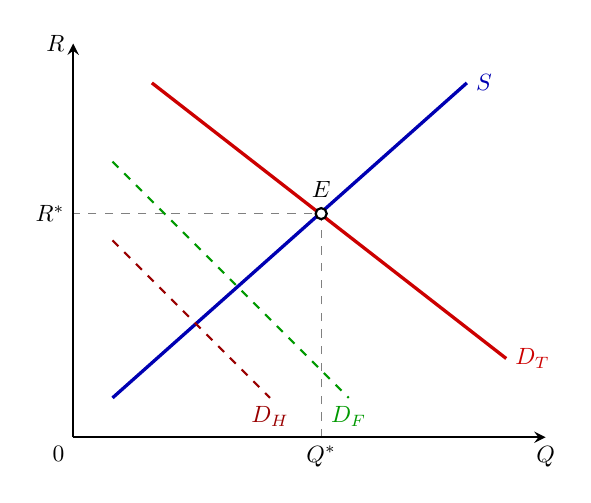
\begin{tikzpicture}[x=1.0cm, y=1.0cm, >=stealth, thick, every node/.style={scale=0.85}]
				% 1. 全局辅助虚线
				\draw[dashed, gray, thin] (3.15,0) -- (3.15,2.84) -- (0,2.84);
				
				% 2. 坐标轴
				\draw[->] (0,0) -- (6.0,0) node[below] {$Q$};
				\draw[->] (0,0) -- (0,5.0) node[left] {$R$};
				\node[below left] at (0,0) {$0$};
				
				% 3. 供需实线
				\draw[very thick, blue!70!black] (0.5,0.5) -- (5.0,4.5) node[right] {$S$};
				\draw[thick, red!60!black, dashed] (0.5,2.5) -- (2.5,0.5) node[below] {$D_H$};
				\draw[thick, green!60!black, dashed] (0.5,3.5) -- (3.5,0.5) node[below] {$D_F$};
				\draw[very thick, red!80!black] (1.0,4.5) -- (5.5,1.0) node[right] {$D_T$};
				
				% 4. 交点与防重叠标签
				\coordinate (E) at (3.15,2.84);
				\fill[white] (E) circle (2pt);
				\draw (E) circle (2pt);
				\node[above, yshift=3pt] at (E) {$E$};
				\node[left] at (0,2.84) {$R^*$};
				\node[below] at (3.15,0) {$Q^*$};
			\end{tikzpicture}
		\end{center}
	\end{enumerate}
	\newpage
	\section{练习题}
	\begin{enumerate}[label=\textbf{\arabic*.}, leftmargin=*]
		\item \textbf{假设利率是 $10\%$ 。如果今天以这个利率投资 100 美元，一年之后它将值多少？两年之后呢？五年之后呢？一年之后支付的 100 美元，今天值多少？两年之后支付的 100 美元，今天值多少？五年之后支付的 100 美元，今天值多少？}
		
		\textbf{答：}
		根据复利终值计算公式，今天投资 100 美元在不同期限后的终值分别为
		\[
		\begin{aligned}
			\text{FV}_1 &= 100 \times (1 + 10\%)^1 = 110.00 \text{（美元）} \\
			\text{FV}_2 &= 100 \times (1 + 10\%)^2 = 121.00 \text{（美元）} \\
			\text{FV}_5 &= 100 \times (1 + 10\%)^5 = 161.05 \text{（美元）}
		\end{aligned}
		\]
		
		根据现值折现公式，未来不同年份支付的 100 美元折算到今天的现值分别为
		\[
		\begin{aligned}
			\text{PDV}_1 &= \frac{100}{(1 + 10\%)^1} = 90.91 \text{（美元）} \\
			\text{PDV}_2 &= \frac{100}{(1 + 10\%)^2} = 82.64 \text{（美元）} \\
			\text{PDV}_5 &= \frac{100}{(1 + 10\%)^5} = 62.09 \text{（美元）}
		\end{aligned}
		\]
		
		\item \textbf{你可以在两种支付流中选择其一：①一年后支付 150 美元，两年后再支付 150 美元；②一年后支付 130 美元，两年后支付 160 美元。当利率为 $5\%$ 时你会选择哪种支付流？ $15\%$ 时呢？}
		
		\textbf{答：}
		理性跨期决策的标准是挑选总现值更高的支付流。设方案一的现值为 $\text{PDV}_a$，方案二的现值为 $\text{PDV}_b$。
		
		当市场利率为 $5\%$ 时，两种支付流的现值分别计算为
		\[
		\begin{aligned}
			\text{PDV}_a &= \frac{150}{1.05^1} + \frac{150}{1.05^2} = 278.91 \text{（美元）} \\
			\text{PDV}_b &= \frac{130}{1.05^1} + \frac{160}{1.05^2} = 268.93 \text{（美元）}
		\end{aligned}
		\]
		由于满足 $\text{PDV}_a > \text{PDV}_b$，在此利率下应当选择方案一。
		
		当市场利率上升至 $15\%$ 时，由于近远期贴现惩罚加重，两种支付流的现值降低为
		\[
		\begin{aligned}
			\text{PDV}_a &= \frac{150}{1.15^1} + \frac{150}{1.15^2} = 243.86 \text{（美元）} \\
			\text{PDV}_b &= \frac{130}{1.15^1} + \frac{160}{1.15^2} = 234.03 \text{（美元）}
		\end{aligned}
		\]
		由于依然满足 $\text{PDV}_a > \text{PDV}_b$，因此在 $15\%$ 的高利率环境下仍然应当选择方案一。
		
		\item \textbf{假定利率是 $10\%$ 。一种有息债券在未来五年内每年支付 80 美元，并在第六年偿还 1000 美元本金，它的价值是多少？若利率是 $15\%$ ，它的价值是多少？}
		
		\textbf{答：}
		根据资产定价模型，有息债券的期初价值等于存续期内各期年息的现值与期末到期本金现值的代数加总。
		
		当市场利率为 $10\%$ 时，该债券的现值计算为
		\[
		\text{PDV} = \sum_{t=1}^5 \frac{80}{(1 + 0.1)^t} + \frac{1000}{(1 + 0.1)^6} \approx 867.73 \text{（美元）}
		\]
		
		当市场利率上升至 $15\%$ 时，由于贴现率分母增大，该债券的市场价值发生跨期减损
		\[
		\text{PDV} = \sum_{t=1}^5 \frac{80}{(1 + 0.15)^t} + \frac{1000}{(1 + 0.15)^6} \approx 700.50 \text{（美元）}
		\]
		\newpage
		
		\item \textbf{一种债券期限为两年。它在一年后支付 100 美元的债息，并在两年后支付 100 美元的债息和 1000 美元的本金。债券以 966 美元出售。它的有效收益率是多少？}
		
		\textbf{答：}
		有效收益率是使债券未来所有资产流的现值之和恰好等于当前市场购买价格的贴现率。根据有息债券的定价方程，可以构建如下关系式
		\[
		P = \frac{C_1}{1+R} + \frac{C_2 + M}{(1+R)^2}
		\]
		将债券市场价格 $P = 966$、首年债息 $C_1 = 100$、次年债息 $C_2 = 100$ 以及期末本金 $M = 1000$ 代入上式中
		\[
		966 = \frac{100}{1+R} + \frac{1100}{(1+R)^2}
		\]
		
		为了求解该方程，在等式两边同乘以 $(1+R)^2$ 并进行代数展开与项合并，可得到关于 $R$ 的标准一元二次方程
		\[
		966R^2 + 1832R - 234 = 0
		\]
		利用求根公式进行计算，并舍去不符合经济学实际意义的负根，可最终求得有效收益率 $R = 0.12$。因此，该债券的内含有效收益率为 $12\%$。
		
		\item \textbf{方程（15.5）显示了对一家电机厂投资的净现值，其中 1000 万美元成本的一半是在一开始就支付的，另一半是在一年后支付，工厂在前两年里预期会赔钱。如果贴现率是 4\%，净现值是多少？投资是否值得？}
		
		\textbf{答：}
		评估该电机厂投资项目的核心在于将各个时点上非均匀分布的现金流统一折现到期初。将给定的市场贴现率 $R = 4\%$ 代入项目的跨期净现值表达式中
		\[
		\begin{aligned}
			\text{NPV} = &-5 - \frac{5}{1.04} - \frac{1}{1.04^2} - \frac{0.5}{1.04^3} \\
			&+ \sum_{t=4}^{20} \frac{0.96}{1.04^t} + \frac{1}{1.04^{20}}
		\end{aligned}
		\]
		
		通过对前期的亏损现金流进行分项折现，并对中后期的年金流运用等比数列求和公式进行加总，可以精确计算出该投资项目的综合净现值
		\[
		\text{NPV} \approx -0.338 \text{（百万美元）}
		\]
		由于该项目的风险调整净现值严格小于零，意味着该工厂创造的未来收益无法覆盖其初始资本投入与跨期机会成本。因此，该项投资在经济学上是不值得的。
		\newpage
		\item \textbf{市场利率是 $5\%$ ，并预期会维持在这个水平上。消费者能以这个利率借入和贷出所有他们想要借贷的金额。在下列每种情况下，解释你的选择：}
		\par \textbf{（1）你是要今天的 500 美元礼金，还是要一年后的 540 美元礼金？}
		\par \textbf{（2）你是要现在的 100 美元礼金，还是要 500 美元四年期的无息贷款？}
		\par \textbf{（3）你在购买一辆 8000 美元的汽车时，是愿意减 350 美元的价钱，还是以零利率贷款一年全价支付？}
		\par \textbf{（4）假定你赢得了“百万美元彩票”。你将在未来的 20 年里每年得到 50000 美元。这在今天对你来说值多少？}
		\par \textbf{（5）你赢得了“诚实的百万”头奖。你可以今天拿 100 万美元，也可以每年拿 60000 美元，永远拿下去（这一权利可以传给你的继承人）。你选择哪一种？}
		\par \textbf{（6）过去，一个成年孩子若从她的父母那里得到超过 10000 美元的礼品，还得要缴税，但是父母可以向他们的孩子贷款而不收利息。为什么某些人认为这一规则不公平？这一规则对谁不公平？}
		
		\textbf{答：}
		针对第一种情况，需要对比两笔礼金在当期的现值。一年后 540 美元礼金的现值可以通过折现公式计算为
		\[
		\text{PDV} = \frac{540}{1 + 0.05} = 514.29 \text{（美元）}
		\]
		由于 $514.29 > 500$，有远见的理性消费者应当选择一年后的 540 美元礼金。
		
		针对第二种情况，四年期无息贷款本质上相当于在期初获得 500 美元，并在第四年末归还 500 美元。该无息贷款由于免除了利息成本，其给消费者带来的净现值红利为
		\[
		\text{NPV}_{\text{贷款}} = 500 - \frac{500}{(1+0.05)^4} = 88.65 \text{（美元）}
		\]
		由于贷款创造的财富红利小于现金礼金的直接价值（$88.65 < 100$），因此应当选择现在的 100 美元礼金。
		
		针对第三种情况，应当比较两种方案下购买汽车所支付的总成本现值，并遵循成本最小化原则。若接受价款折让，当前的实际支出成本现值为
		\[
		\text{PDV}_{\text{折扣}} = 8000 - 350 = 7650 \text{（美元）}
		\]
		若选择一年期零利率贷款全价支付，意味着在第一年末才需要支付 8000 美元，其成本现值为
		\[
		\text{PDV}_{\text{贷款}} = \frac{8000}{1+0.05} = 7619.05 \text{（美元）}
		\]
		由于延迟支付降低了资金的跨期机会成本，满足 $\text{PDV}_{\text{贷款}} < \text{PDV}_{\text{折扣}}$，因此应当选择零利率贷款方案。
		
		针对第四种情况，该彩票属于首期立即支付的即付年金组合。将未来 20 年每年流入的 50000 美元全部折现，为了防止公式溢出，将其切分为多行表达
		\[
		\begin{aligned}
			\text{PDV} &= \sum_{t=0}^{19} \frac{50000}{(1+0.05)^t} \\
			&= 50000 \times \left[ \frac{1 - (1.05)^{-20}}{0.05} \right] \times 1.05 \\
			&= 654266.04 \text{（美元）}
		\end{aligned}
		\]
		
		针对第五种情况，无限期发放且可继承的年金在数理上构成了一笔永续年金资产。该永续年金流在当期所对应的总资产现值可以通过如下公式求得
		\[
		\text{PDV}_{\text{永续}} = \frac{W}{R} = \frac{60000}{0.05} = 1200000 \text{（美元）}
		\]
		由于永续年金的总折现价值显著高于直接结算的当期现金（$1200000 > 1000000$），因此应当选择每年拿 60000 美元。
		
		针对第六种情况，免息贷款实质上充当了规避赠予税的隐性财富转移工具。如果父母希望向孩子进行一笔数额为 $N$ 的隐性免税赠予，只需向孩子提供一笔数额为 $L$ 的大额无息贷款，其数理对应关系为
		\[
		L = \frac{N(1+R)}{R}
		\]
		孩子将这笔资金存入市场获取利息，即可在期末无税获得相当于 $N$ 的财富变现。
		
		例如，若想免税转移 50000 美元，富裕家庭只需无息借给孩子 1050000 美元即可。由于这种高额资金拆借需要极强的流动性支持，普通低收入家庭根本无法利用该漏洞。因此，这一规则对普通薪资家庭是不公平的，实质上恶化了阶层间的财富代际分配。
		
		\item \textbf{拉尔夫正试图决定是否去读研究生。如果他花两年时间读研究生，每年支付 15000 美元的学费，他可以在他以后的工作时间里得到每年 60000 美元的工作。如果他不去读研究生，他将立即参加工作。他将在最初三年里每年得到 30000 美元，在接着的三年里每年得到 45000 美元，并在此后每年得到 60000 美元。如果利息率是 $10\%$ ，读研究生是不是一项好的金融投资？}
		
		\textbf{答：}
		由于在第 6 年之后，无论拉尔夫是否选择攻读研究生学位，其未来的年度市场薪资报酬均对称稳定在 60000 美元，因此在跨期决策中，第 6 年之后的现金流属于不相关成本，可以进行代数对冲。我们只需定量对比前 6 年两种决策路径下的总回报现值。
		
		若拉尔夫决定攻读研究生，前两年的学费作为现金流出，后四年的高额薪资作为现金流入。假定所有收支均在年末发生，该决策路径的总现值 $\text{PDV}_1$ 计算为
		\[
		\begin{aligned}
			\text{PDV}_1 &= \sum_{t=1}^2 \frac{-15000}{(1.1)^t} + \sum_{t=3}^6 \frac{60000}{(1.1)^t} \\
			&= 131150.35 \text{（美元）}
		\end{aligned}
		\]
		
		若拉尔夫选择直接参加工作，前三年与后三年分别获得不同阶梯的劳动报酬，期间不存在任何学费的流出。该直接就业决策路径的总现值 $\text{PDV}_2$ 计算为
		\[
		\begin{aligned}
			\text{PDV}_2 &= \sum_{t=1}^3 \frac{30000}{(1.1)^t} + \sum_{t=4}^6 \frac{45000}{(1.1)^t} \\
			&= 158683.95 \text{（美元）}
		\end{aligned}
		\]
		
		通过对两组跨期总现值进行比较，可以清晰地发现直接参加工作的财富现值显著更高
		\[
		\text{PDV}_2 > \text{PDV}_1
		\]
		攻读研究生不仅需要支付高昂的直接学费，更造成了高额的早期误工机会成本。在高利率环境下，早期的现金流入具有更高的权重，因此从纯粹的金融投资视角来看，读研究生并不是一项明智的经济决策。
		\newpage
		\item \textbf{假定你的叔叔给了你一口像教材第 15.8 节中描述的油井（边际生产成本是不变的 50 美元）。当前的石油价格是 80 美元，但它受到一个卡特尔的控制，该卡特尔占了总生产的一个很大的比重。你应当现在生产和销售你的石油，还是等待以后再生产？解释你的答案。}
		
		\textbf{答：}
		根据可耗竭资源的开采原则，若预期价格扣除开发成本后的净收益增速快于利率，则应留存资源；若增速慢于利率，则应立即开采销售。
		
		在卡特尔垄断控制的市场中，垄断者为实现总利润现值最大化，会控制产量使边际收益扣除边际成本后的净额随利率增长。
		
		由于资源价格大于边际收益，价格扣除边际成本后的开采净利润其增长速度必然低于市场利率。
		
		因此，当前开采并销售石油能够获得更高的资产净现值，应当选择现在生产和销售。相关开采决策的代数判别式可以表述为：
		\[
		P_{t+1} - C < (1 + R)(P_t - C)
		\]
		
		\item \textbf{你计划投资于优质葡萄酒。每箱成本为 100 美元，而你根据经验知道，每箱葡萄酒保存 $t$ 年后的价值为 $100t^{0.5}$ 。现有 100 箱酒可销售。并且利率是 $10\%$ 。\\（1）你应当买多少箱，等待多久再出售它们，并且你在出售它们的时候能够得到多少钱？\\（2）假定在购买的时候，有人立即开价每箱 130 美元。你应当接受这个价格吗？\\（3）如果利率只有 5\%，你的回答有什么变化？}
		
		\textbf{答：}
		对于第一问，购买优质葡萄酒的单箱净现值公式由购买成本与未来销售收入的折现值共同决定。
		
		为了实现投资收益最大化，对单箱净现值函数关于时间求一阶导数并令其为零，从而确定最佳留存年限。
		\[
		\begin{aligned}
			\text{净现值} &= -100 + e^{-0.1t} \cdot 100t^{0.5} \\
			\frac{\text{d}\text{净现值}}{\text{d}t} &= e^{-0.1t} \left(50t^{-0.5}\right) - 0.1e^{-0.1t} \cdot 100t^{0.5} = 0
		\end{aligned}
		\]
		
		解得最佳销售时间为 5 年。此时单箱净现值为 35.62 美元。由于每箱均能获利，应当买下全部 100 箱酒。
		
		在第 5 年出售时，每箱实际价值为 223.61 美元，因此 100 箱酒在出售时总共能得到 22361 美元（总净现值为 3562 美元）。
		
		对于第二问，若立即以 130 美元卖出，单箱锁定的当期利润仅为 30 美元。
		
		这低于继续保存 5 年所能带来的净现值 35.62 美元，因此不应当接受这个出价。
		
		对于第三问，当市场利率降至 5\% 时，投资的单箱净现值函数及其最优化条件随之发生改变。
		\[
		\begin{aligned}
			\text{净现值} &= -100 + e^{-0.05t} \cdot 100t^{0.5} \\
			\frac{\text{d}\text{净现值}}{\text{d}t} &= e^{-0.05t} \left(50t^{-0.5}\right) - 0.05e^{-0.05t} \cdot 100t^{0.5} = 0
		\end{aligned}
		\]
		
		此时解得最佳留存时间延长为 10 年，对应的单箱最大净现值大幅提升至 91.80 美元。
		
		因此仍应购买 100 箱酒，等待 10 年后再出售，届时每箱价值为 316.23 美元，总计可获得 31623 美元。
		\newpage
		\item \textbf{从现存厂商的角度再考察一次性纸尿裤产业中的资本投资（教材中例 15.4）。如果宝洁公司或金伯利—克拉克公司通过再建三个新工厂来扩大生产能力，它们在开工之前不必再在研究与开发上花费 6000 万美元。这将如何影响表 15-1 中净现值的计算？在贴现率 12\% 时，这一投资是有利可图的吗？}
		\begin{center}
			\footnotesize
			\setlength{\tabcolsep}{3pt}
			\renewcommand{\arraystretch}{1.2}
			\begin{tabular}{lccccccc}
				\hline
				& 2010年前 & 2010 & 2011 & 2012 & $\dots$ & 2025 \\ \hline
				销售 & & 133.3 & 266.7 & 400.0 & $\dots$ & 400.0 \\
				减：可变成本 & & 96.7 & 193.3 & 290.0 & $\dots$ & 290.0 \\
				持续研发 & & 20.0 & 20.0 & 20.0 & $\dots$ & 20.0 \\
				销售与广告 & & 50.0 & 50.0 & 50.0 & $\dots$ & 50.0 \\ \hline
				经营利润 & & -33.4 & 3.4 & 40.0 & $\dots$ & 40.0 \\ \hline
				减：建设成本 & 60.0 & 60.0 & 60.0 & & $\dots$ & \\
				初始研发 & 60.0 & & & & $\dots$ & \\ \hline
				净现金流量 & -120.0 & -93.4 & -56.6 & 40.0 & $\dots$ & 40.0 \\ \hline
				贴现率 & & 0.05 & 0.10 & 0.15 & $\dots$ & \\
				净现值 & & 80.50 & -16.90 & -75.10 & $\dots$ & \\ \hline
			\end{tabular}
		\end{center}
		
		\textbf{答：}
		现存厂商因为无需重复投入初始研究开发费，各期现金流中的初始研发费减少 60 百万美元。
		
		这意味着在任何贴现率下，整个投资方案的净现值都会在原先基础上面直接增加 60 百万美元。
		
		调整后的不同贴现率与净现值对应关系如表格所示：
		\begin{center}
			\small
			\setlength{\tabcolsep}{8pt}
			\renewcommand{\arraystretch}{1.2}
			\begin{tabular}{lccc}
				\hline
				贴现率 & 0.05 & 0.10 & 0.15 \\ \hline
				净现值（百万美元） & 140.50 & 43.10 & -15.10 \\ \hline
			\end{tabular}
		\end{center}
		
		当贴现率为 12\% 时，我们可以将各期的现金流进行逐期折现加总，从而精确算出新的总净现值。
		\[
		\text{净现值} = -60 - \frac{93.4}{1.12} - \frac{56.6}{1.12^2} + \frac{40}{1.12^3} + \frac{40}{1.12^4} + \dots + \frac{40}{1.12^{16}} = 16.30
		\]
		
		由于在 12\% 的贴现率下计算出的净现值大于零，因此该现存厂商扩大生产能力的投资方案是有利可图的。
		
		\item \textbf{假设你可以以 2 万美元购买了一辆丰田卡罗拉，并且六年之后出售，仍可得到 1.2 万美元。另一个方案是，你可以以每月 300 美元的价格租用三年，到期将车退还。为了简单起见，假定租金是以年支付而不是以月支付——比如，三年中每年交纳 3600 美元。\\（1）如果利率为 4\%，租车是不是比买车好？\\（2）如果利率为 12\%，哪种方式更好？\\（3）利率为多少时，在购买和租用之间无差异？}
		
		\textbf{答：}
		在利率为 4\% 时，分别计算购买汽车与租用汽车在相应跨度内的现金流转现值。
		\[
		\begin{aligned}
			\text{买车净现值} &= -20000 + \frac{12000}{1.04^6} = -10516.22 \\
			\text{租车净现值} &= -3600 - \frac{3600}{1.04} - \frac{3600}{1.04^2} = -10389.94
		\end{aligned}
		\]
		
		比较可知租车的流出总现值较低，因此选择租车方案更为划算。
		
		在利率为 12\% 时，较高的贴现率会使未来的资产回收价值发生显著缩水，需要重新评估两套方案。
		\[
		\begin{aligned}
			\text{买车净现值} &= -20000 + \frac{12000}{1.12^6} = -13920.43 \\
			\text{租车净现值} &= -3600 - \frac{3600}{1.12} - \frac{3600}{1.12^2} = -9684.18
		\end{aligned}
		\]
		
		此时租车的成本现值优势进一步扩大，因此依然应当选择租车方案。
		
		无差异意味着两种方案的现金流折现总额完全相等，可以通过建立关于无风险利率的等式来求解。
		\[
		-20000 + \frac{12000}{(1+r)^6} = -3600 - \frac{3600}{1+r} - \frac{3600}{(1+r)^2}
		\]
		
		通过对不同利率水平下的两套方案净现值进行试算对比，可以得出其变化趋势。
		\begin{center}
			\small
			\setlength{\tabcolsep}{8pt}
			\renewcommand{\arraystretch}{1.2}
			\begin{tabular}{ccc}
				\hline
				利率 $r$ & 买车净现值 & 租车净现值 \\ \hline
				0.030 & -9950.19 & -10488.49 \\
				0.035 & -10237.99 & -10438.90 \\
				0.037 & -10350.41 & -10419.24 \\
				0.038 & -10406.06 & -10409.44 \\
				0.039 & -10461.33 & -10399.68 \\
				0.040 & -10516.22 & -10389.94 \\ \hline
			\end{tabular}
		\end{center}
		
		根据测算结果，当利率约为 3.8\% 时，买车与租车的净现值基本相等，消费者在此处无差异。
		
		\item \textbf{一个消费者面临如下决策：她可以以 1000 美元购买一台电脑并且在接下来三年中每月支付 10 美元的网费；或者接受 400 美元的折扣（因此购买成本是 600 美元）但在接下来的三年内每月支付 25 美元的网费。为了简化起见，假设消费者是以年支付网费（就是说，10 美元/月=120 美元/年）。\\（1）如果利率为 3\%，消费者该如何决策？\\（2）如果利率为 17\% 时那？\\（3）利率为多少时，消费者对两种选择是无差异的？}
		
		\textbf{答：}
		当市场利率为 3\% 时，分别将两种网费支付方案下的购买成本与年网费支出进行折现加总。
		\[
		\begin{aligned}
			\text{第一种方案净现值} &= -1000 - 120 - \frac{120}{1.03} - \frac{120}{1.03^2} = -1349.62 \\
			\text{第二种方案净现值} &= -600 - 300 - \frac{300}{1.03} - \frac{300}{1.03^2} = -1474.04
		\end{aligned}
		\]
		
		第一种方案的现金流出总现值更低，因此应当选择花 1000 美元买电脑并支付较低网费的方案。
		
		当市场利率大幅上升至 17\% 时，未来高额网费支出的资本化现值会下降，需重新核算流出总额。
		\[
		\begin{aligned}
			\text{第一种方案净现值} &= -1000 - 120 - \frac{120}{1.17} - \frac{120}{1.17^2} = -1310.23 \\
			\text{第二种方案净现值} &= -600 - 300 - \frac{300}{1.17} - \frac{300}{1.17^2} = -1375.56
		\end{aligned}
		\]
		
		两相比较，第一种方案依然具有明显的成本优势，消费者仍然应该维持原有的购买决策。
		
		当两套方案的流出总现值完全相等时，消费者达到无差异状态，可据此列出代数方程。
		\[
		-1000 - 120 - \frac{120}{1+r} - \frac{120}{(1+r)^2} = -600 - 300 - \frac{300}{1+r} - \frac{300}{(1+r)^2}
		\]
		
		对方程进行各项同类项合并与化简后，可以得到关于利率的一元二次方程。
		\[
		220r^2 + 260r - 140 = 0
		\]
		
		求解该方程可得正根为 40.2\%。因此当市场利率达到 40.2\% 时，两套方案对消费者而言完全等价。
	\end{enumerate}
		
	